\documentclass[11pt,reqno]{amsart}

\usepackage{amsmath,amssymb,amsthm,mathtools}
\usepackage{tikz}
\usetikzlibrary{shapes.geometric, positioning, arrows.meta, decorations.pathmorphing, patterns}
\usepackage{array,booktabs,tabularx,float}
\usepackage[hidelinks]{hyperref}

\allowdisplaybreaks
\raggedbottom
\setlength{\emergencystretch}{2em}

\newtheorem{theorem}{Theorem}[section]
\newtheorem{proposition}[theorem]{Proposition}
\newtheorem{lemma}[theorem]{Lemma}
\newtheorem{corollary}[theorem]{Corollary}
\theoremstyle{definition}
\newtheorem{definition}[theorem]{Definition}
\newtheorem{example}[theorem]{Example}
\newtheorem{warning}[theorem]{Warning}
\newtheorem{openproblem}[theorem]{Open Problem}
\theoremstyle{remark}
\newtheorem{remark}[theorem]{Remark}

\newcommand{\C}{\mathbb C}
\newcommand{\Z}{\mathbb Z}
\newcommand{\Chat}{\widehat{\mathbb C}}
\newcommand{\Fill}{\operatorname{Fill}}
\newcommand{\Exp}{\operatorname{Exp}}
\newcommand{\Int}{\operatorname{int}}
\newcommand{\dist}{\operatorname{dist}}
\newcommand{\id}{\operatorname{id}}
\newcommand{\Om}{\Omega}
\newcommand{\Omfree}{\Omega_{\mathrm{free}}}
\newcolumntype{P}[1]{>{\raggedright\arraybackslash}p{#1}}
\newcolumntype{Y}{>{\raggedright\arraybackslash}X}

\title[Protected planar carriers]{Protected planar carriers:\\
separation ledgers and access-preserving routing}
\author{Matthew Robert Wesney}
\date{Draft II of 2026-07-27}
\subjclass[2020]{Primary 54F15, 30C20; Secondary 37F20, 55M05}
\keywords{plane continuum, prime end, Alexander duality, protected access,
connector, filled hull, Hausdorff limit}
\hypersetup{
  pdftitle={Protected planar carriers: separation ledgers and access-preserving routing},
  pdfauthor={Matthew Robert Wesney},
  pdfsubject={Planar continuum theory and access-preserving routing},
  pdfkeywords={plane continuum, prime end, Alexander duality, protected access,
    connector, filled hull, Hausdorff limit}
}

\begin{document}

\begin{abstract}
We give a finite planar theory for joining pairwise disjoint full continua
while preserving specified prime-end accesses and avoiding a frozen compact
inventory.  A protected ribbon-routing certificate is realized by a full
carrier whose null crosscut chains survive, remain distinct when their
relative collar tails are disjoint, and retain cyclic order, without any
local-connectivity hypothesis.  Certificate existence is equivalent to one
component of the frozen free domain admitting simultaneous singleton ports
to all atoms.  Packet and cellwise criteria give checkable sufficient
conditions, while fixed-assignment audits give persistent witnesses for
merger, escape, and port loss.

We also prove an attachment exact sequence.  If a connected connector $C$
meets a full atom $A$ in $T$, then the new first \v{C}ech cohomology fits into
the short exact sequence
$0\to\widetilde{\check H}^{\,0}(T)\to
\check H^1(C\cup A)\to
\ker[\check H^1(C)\to\check H^1(T)]\to0$.
Iteration gives the separation ledger
\[
\sigma\!\left(C\cup\bigcup_iA_i\right)
=\sigma(C)+\sum_i
\bigl(\#\pi_0(C\cap A_i)-1-\sigma(C\cap A_i)\bigr)
\]
whenever the ranks are finite.  Thus disconnected traces create holes and
separating traces fill pre-existing holes.  For a full connector the union
is full exactly when every attachment trace is connected.  Arbitrarily many
holes can nevertheless be born in a Hausdorff limit of full tree carriers
with singleton traces.  By contrast, decreasing full connector envelopes
with nonempty connected traces are stable and preserve common protected
data.
These results isolate the precise finite/infinite compactness gate; they make
no claim of constructing a virtual dynamical carrier or proving Mandelbrot
local connectivity.
\end{abstract}

\maketitle
\tableofcontents

% ---- begin A:intro_v2 ----
% Draft-II introduction: paper-level architecture centered on the planar theory.

\section{Introduction}\label{sec:intro}

\subsection{The routing problem}

Let $s\ge1$, and let $A_1,\dots,A_s$ be pairwise disjoint full continua in a Jordan disk
$U\subset\C$.  The elementary task of joining the $A_i$ becomes substantially
less elementary when the connector must also avoid a frozen compact obstacle
set and preserve designated prime ends of the complements
$\Chat\setminus A_i$.  A connector can erase such an access by entering its
selected side, identify two accesses that were distinct before enlargement,
or disconnect the region through which later ports were meant to run.
None of these failures is detected by connectedness of the final union.

This problem appears naturally when small filled Julia sets, puzzle pieces,
or combinatorial fibers must be organized without assuming local
connectivity.  Polynomial-like maps provide the basic continua
\cite{DH85}; Kahn--Lyubich impose finite-decoration combinatorics and
prove a~priori bounds for that class \cite{KL08}; recent work on
primitive renormalization constructs native or model-lifted Hubbard trees
when the required dynamical structure is available \cite{KKL26}; and
Dudko's roadmap emphasizes connected hulls of families of small Julia sets
as one ingredient in the broader local-connectivity program \cite{Dud25}.
The present paper isolates the planar problem that remains after the
dynamical data have selected finitely many continua and accesses but before
any canonical connector has been justified.

The hypotheses deliberately allow non-locally-connected boundaries.
A protected access is therefore not represented by a presumed landing ray
or boundary parametrization.  It is represented by a null prime-end
crosscut chain together with its selected sides.  The part forbidden to a
future connector is the \emph{relative collar tail}
$\overline D\setminus A_i$, not the whole closed side $\overline D$.
This distinction is essential: different prime ends may have overlapping
impressions inside the same atom even though their relative collar tails in
the complement are disjoint.

\subsection{Main results}

The first conclusion is negative but foundational.  There is no least
compact connected full hull even for two points
(Theorem~\ref{thm:no-least}), so ``take the smallest carrier'' is not a
definition.  Nor can one safely choose a carrier and absorb pulled-back
excess monotonically: Proposition~\ref{prop:access-collision} gives a
degree-one conformal branch, with no critical-value obstruction, in which
the first absorption erases a protected access permanently.  These examples
show that the isotopy/access class of the routing is additional data.

The positive replacement is a \emph{protected ribbon-routing certificate}.
It records free singleton ports from the atoms, a finite embedded tree
joining their outer endpoints, the induced ribbon order, every protected
crosscut chain, and the complete frozen inventory to be avoided.
Theorem~\ref{thm:realization} realizes any such certificate by a compact
connected full carrier.  Every protected chain remains a prime-end chain of
the enlarged complement, distinct protected chains remain distinct whenever
their relative collar tails are disjoint, and cyclic order is preserved
within each common source complement.  No local connectivity of an atom is
used.

The first structural result developed here is an exact attachment ledger.
For a compact connected connector $C$, full atoms $A_i$, and traces
$T_i=C\cap A_i$, Theorem~\ref{thm:separation-budget} extracts from the
compact-pair Mayer--Vietoris sequence a natural short exact sequence at
every attachment.  When the relevant component counts are finite, it gives
\[
 \sigma\!\left(C\cup\bigcup_iA_i\right)
 =
 \sigma(C)+
 \sum_i\bigl(\#\pi_0(T_i)-1-\sigma(T_i)\bigr),
\]
where $\sigma(K)=\#\pi_0(\Chat\setminus K)-1$.  The formula is a
credit/debit law.  Each extra component of an attachment trace creates a
complementary component; each complementary component of the trace fills
one separation already present in the connector.  In particular, if $C$
and the atoms are full, every $T_i$ is nonseparating and the union is full
if and only if all traces are connected
(Corollary~\ref{cor:full-connector-traces}).  Thus the familiar tree with
singleton attachments is only one sufficient model: an arbitrary full
continuum connector with arbitrary connected traces works just as well.

The same ledger identifies a compactness gate for this framework.
Proposition~\ref{prop:trace-birth} constructs, for every $m$, full arc
connectors $C_n$ meeting an atom once and converging in the Hausdorff metric
to a full arc $C$ whose trace has $m+1$ components.  Each finite-stage
union $A\cup C_n$ is full, while the
limit union has exactly $m$ bounded complementary components.
Connector cycles can likewise be born in a limit.  Consequently neither
fullness nor the singleton-trace condition passes to a virtual or infinite
carrier by Hausdorff compactness alone: a limiting argument must separately
control connector cohomology and trace multiplication
(Warning~\ref{warn:compactness-gate}).  Theorem
\ref{thm:nested-limit-stability} gives a positive counterpart: a decreasing
sequence of full connector envelopes with connected nonempty traces has a
full limiting connector with connected traces, and common protected data
survive.  This identifies a concrete inverse-limit architecture that avoids
both defect-birth mechanisms.

The second structural result is an exact routing criterion.  Freeze the
atoms, relative protected collar tails, obstacles, critical exclusions, and
localization-forbidden data into a compact set $Q$, and put
$\Omfree=U\setminus Q$.  Theorem~\ref{thm:free-component} says that a
protected certificate exists if and only if one component of $\Omfree$
admits simultaneous singleton ports to every required atom.  If no
component of this fixed free domain has simultaneous ports, the failure
persists under every connector enlargement respecting the same $Q$.  The
proof uses a one-ended slit lemma whose statement keeps
the free tips inside the residual domain.  The source version deleted those
tips and mapped a boundary-anchored slit into an open domain; the corrected
Lemma~\ref{lem:slits} repairs both defects, and the proof of the criterion is
rebuilt around the repaired statement.

Finally, the exact criterion is converted into finite audits.
Theorem~\ref{thm:common-domain} packages the frozen inventory into pairwise
disjoint full continua and uses compacta Alexander duality to force a common
free domain.  Theorem~\ref{thm:audit} proves that fullification is independent
of processing order for a fixed typed assignment and reduces success to
coverage, packet separation/localization, and a nonempty unprotected
exposure locus at each atom.  Packet merger, localization escape, and port
loss come with witnesses persistent under every same-label monotone
enlargement.  Proposition~\ref{prop:cellwise} supplies a directly checkable
Jordan-cell criterion.

\subsection{Position}

The underlying tools are classical: Janiszewski--\allowbreak Mullikin separation
\cite{Jan15,Mul22,New51,Why42}, the classical theories of unicoherence and
multicoherence \cite{Bor31,Eil36}, Carath\'eodory prime ends \cite{Pom92}, the
Jordan--Schoenflies theorem, filled hulls, and compacta Alexander duality and
Mayer--Vietoris \cite[Chapter~6]{Spa66}.  We do not claim a new foundation
for planar topology.  The contribution is a theorem-level synthesis aimed
at a specific proof obligation that the standard constructions do not
record: finite connection with named access survival, exact existence and
failure tests, and a quantitative accounting of the separations created or
destroyed by attachment.

In particular, the separation-ledger theorem is formally a consequence of
classical duality and Mayer--Vietoris; its full/full zero-defect criterion
is part of the Janiszewski--Mullikin tradition.  Its value here is the
homomorphism-level diagnostic, the creation-versus-cancellation formula,
and the limit obstruction it exposes.  The other central statements
turn prime-end intentions into finite data: null chains and relative
collar tails, singleton ports, an embedded ribbon tree, a frozen free domain,
typed packet assignments, and persistent witnesses.  Section
\ref{sec:comparison} compares this package with least hulls, monotone
absorption, regulated and Hubbard trees, Moore quotients, and a
lamination-lift candidate.

This architecture is intentionally distinct from the companion
direct-decoration manuscript \cite{Wes26}.  That manuscript contains the rooted-end
compactification, partial-shift dynamics, gap cells, arbitrary packet
replacement, and the finite decoration-carrier application.  The present
paper contains the general planar certification theory, the exact
free-component and packet criteria, the attachment ledger, and the
Hausdorff-limit no-go theorem.  Separating the two removes a long duplicated
application and makes the logical dependency transparent.

\subsection{Scope and organization}

Everything here is finite and planar.  The paper does not construct a
virtual carrier or ``Wave horizon'' (the source manuscript's proposed
infinite limiting carrier), an analytic correspondence, a uniform
incidence bound, or a compression mechanism, and it proves no new case of
local connectivity of the Mandelbrot set.  The recent theorem of
Kahn--Kapiamba--Lyubich applies in its stated parabolically bounded primitive
category \cite{KKL26}; it is a positive benchmark, not a consequence of the
present framework.  Our conclusion is conditional in exactly one transparent
sense: once finite protected data or a valid packet assignment are supplied,
the planar realization problem is solved, while the production of coherent
data at an infinite dynamical horizon remains open.

Section~\ref{sec:prelim} fixes the compacta and prime-end conventions.
Section~\ref{sec:obstructions} proves the two motivating obstructions, and
Section~\ref{sec:comparison} places the framework among standard
constructions.  Section~\ref{sec:certificates} gives certificate realization
and prime-end survival.  Section~\ref{sec:separation-budget} proves the
attachment ledger and its sharp Hausdorff-limit obstruction.
Section~\ref{sec:criterion} proves the corrected slit lemma and exact
free-component criterion.  Sections~\ref{sec:packets} and~\ref{sec:audit}
develop the packet criterion, order-independent fullification, persistent
audits, and the cellwise test.  Section~\ref{sec:scope} closes with the exact
interface to future finite and limiting applications.
% ---- end A:intro_v2 ----

% ---- begin A:preliminaries ----
% Cluster A: notation and classical background
% Body-only LaTeX; preamble macros, cite keys, and cross-cluster labels per CONVENTIONS.md.

\section{Notation and classical background}\label{sec:prelim}

Everything in this section is classical.  It is collected once, in the
normalized forms used by the rest of the paper, for three reasons: the
statements are invoked repeatedly and in exact form; two of them --- the
compacta form of Alexander duality and the tameness of plane arcs --- are
easy to quote in weaker versions that would not support the proofs; and the
source manuscript's terminology --- \emph{atom}, \emph{package},
\emph{carrier}, \emph{fullification}, \emph{protected access},
\emph{collar} --- is fixed here at first use.

\subsection{Plane, sphere, and general notation}\label{subsec:A-notation}

Throughout, $\C$ is the complex plane, $\Z$ the integers, and
$\Chat=\C\cup\{\infty\}$ the Riemann sphere, identified with the round
sphere $S^2$ by stereographic projection and carrying its standard
orientation.  Compact subsets of $\C$ are exactly the compact subsets of
$\Chat$ missing $\infty$, and we pass between the two ambient spaces
without comment.  The symbol $\dist$ denotes Euclidean distance in $\C$;
diameters of crosscuts (Section~\ref{subsec:A-primeends}) are measured in
the spherical metric, and all other metric quantities are Euclidean.  For
a set $X$, $\Int X$ is its interior, $\partial X$ its boundary, and
$\overline{X}$ its closure, taken in the ambient space clear from context;
the relative closure of $X$ in a subspace $Y$ is written
$\overline{X}^{\,Y}$, as in the attachment trace \eqref{eq:B-trace}.

For sets $A,B$ we write $A\Subset B$, and say $A$ is \emph{compactly
contained} in $B$, if $\overline{A}$ is compact and
$\overline{A}\subset\Int B$; this is the manuscript's relation~$\Subset$.
A \emph{domain} is a nonempty connected open subset of $\C$ or $\Chat$; a
\emph{plane domain} is a domain in $\C$.  Every plane domain is polygonally
connected: any two of its points are joined by a polygonal path inside it
\cite{New51}.  A \emph{Jordan curve} is a homeomorphic image of the circle,
a \emph{Jordan arc} a homeomorphic image of $[0,1]$, and an \emph{open
Jordan arc} a Jordan arc with its two endpoints removed.  A \emph{Jordan
disk} (synonymously, a \emph{Jordan domain}) is a bounded plane domain
whose boundary is a Jordan curve; by the Jordan and Schoenflies theorems
recalled in Proposition~\ref{prop:A-extension} below, a Jordan disk is
simply connected, and its closure --- a \emph{closed Jordan disk} --- is
homeomorphic to the closed unit disk.  A \emph{continuum} is a nonempty
compact connected subset of $\C$ or $\Chat$; it is \emph{nondegenerate} if
it contains more than one point.

\subsection{Full continua, filled hulls, and fullification}
\label{subsec:A-full}

A compact set $K\subset\C$ is \emph{full} if $\C\setminus K$ is connected.
Following the source manuscript (equation~(9.5) of \cite{MWman}), the
\emph{filled hull} of a compact set $K\subset\C$ is
\begin{equation}\label{eq:A-fill}
\Fill(K)\;=\;K\,\cup\,
\bigcup\bigl\{\,B : B \text{ a bounded component of }\C\setminus K\,\bigr\},
\end{equation}
that is, $K$ together with the bounded components of its complement.  The
passage from $K$ to $\Fill(K)$ is called \emph{fullification}; the term is
the manuscript's, and it is used as a noun for the operation and,
occasionally, for its result.  The following properties are used
constantly and are recorded with proof.

\begin{lemma}[Basic properties of filled hulls]\label{lem:A-full}
Let $K\subset\C$ be compact, and let $\Omega_\infty(K)$ denote the
unbounded component of $\C\setminus K$.
\begin{enumerate}
\item $\Fill(K)=\C\setminus\Omega_\infty(K)$; in particular $\Fill(K)$ is
compact, and it is contained in every closed disk containing $K$.
\item The following are equivalent: $K$ is full; $\Chat\setminus K$ is
connected; $\Fill(K)=K$.
\item If $K$ is a continuum, then $\Fill(K)$ is a full continuum, and
$\Chat\setminus\Fill(K)=\Omega_\infty(K)\cup\{\infty\}$ is a simply
connected domain containing $\infty$.
\item The operator $\Fill$ is extensive ($K\subset\Fill(K)$), monotone
($K\subset L$ implies $\Fill(K)\subset\Fill(L)$), and idempotent
($\Fill(\Fill(K))=\Fill(K)$).
\end{enumerate}
\end{lemma}

\begin{proof}
(1) The set $\C\setminus\Omega_\infty(K)$ consists of $K$ together with
all bounded components of $\C\setminus K$, which is \eqref{eq:A-fill}; it
is closed because $\Omega_\infty(K)$ is open.  If $E$ is a closed disk with
$K\subset E$, then $\C\setminus E$ is a connected unbounded subset of
$\C\setminus K$, hence contained in $\Omega_\infty(K)$; taking complements
gives $\Fill(K)\subset E$.  Thus $\Fill(K)$ is closed and
bounded.

(2) The components of $\Chat\setminus K$ are the bounded components of
$\C\setminus K$ together with $\Omega_\infty(K)\cup\{\infty\}$: the latter
set is open in $\Chat$ (a spherical neighborhood of $\infty$ misses the
compact set $K$, and its intersection with $\C$, being connected and
unbounded, lies in $\Omega_\infty(K)$), it is connected, and its
complement within $\Chat\setminus K$ is the union of the bounded
components, which is open.
Hence $\Chat\setminus K$ is connected exactly when there are no bounded
components, which is fullness of $K$, which by \eqref{eq:A-fill} is the
identity $\Fill(K)=K$.

(3) Let $K$ be a continuum and let $B$ be a bounded component of
$\C\setminus K$.  The boundary of $B$ is contained in $K$: if a boundary
point $x$ of $B$ lay in $\C\setminus K$, its component $B'$ in
$\C\setminus K$ would be an open set containing $x$, hence meeting $B$,
hence equal to $B$; but then $x\in B$, contradicting openness of $B$ at
its own boundary point.  So $\partial B\subset K$.  Thus $\overline{B}=B\cup\partial B$ is a
connected set meeting $K$, and
$\Fill(K)=K\cup\bigcup_B\overline{B}$ is a union of connected sets each
meeting the connected set $K$, hence connected.  With (1) this makes
$\Fill(K)$ a continuum, and its complement in $\Chat$ is the domain
$\Omega_\infty(K)\cup\{\infty\}$, so $\Fill(K)$ is full.  Finally, a
domain in $\Chat$ whose complement is connected is simply connected
\cite{New51,Why42}, and the complement of the domain
$\Omega_\infty(K)\cup\{\infty\}$ is the continuum $\Fill(K)$.

(4) Extensivity is \eqref{eq:A-fill}.  For monotonicity, let
$K\subset L$; then $\Omega_\infty(L)$ is a connected unbounded subset of
$\C\setminus K$, hence $\Omega_\infty(L)\subset\Omega_\infty(K)$, and
taking complements in (1) gives $\Fill(K)\subset\Fill(L)$.  For
idempotence, the complement of $\Fill(K)$ is the single unbounded
component $\Omega_\infty(K)$, so $\Fill(\Fill(K))=\C\setminus
\Omega_\infty(K)=\Fill(K)$.
\end{proof}

The deeper absorption law
$\Fill(\Fill(K)\cup L)=\Fill(K\cup L)$, which makes fullification of a
typed packet independent of processing order, is
Lemma~\ref{lem:fill-absorption} below (manuscript Lemma~10.12); it is a
formal consequence of the three properties in clause~(4).

\begin{definition}[Package, atoms, carrier, fullification]
\label{def:A-package}
A \emph{package} is a nonempty finite union
$S=A_1\cup\dots\cup A_s$, $s\ge1$, of pairwise disjoint full continua,
called its \emph{atoms}.  Atoms may be
degenerate: in Theorem~\ref{thm:no-least} the package consists of the two
points $\pm1$.  A \emph{carrier} of the package $S$ is a compact
connected full continuum $H\subset\C$ with $S\subset H$.  Both
\emph{atom} --- a required full continuum of the package --- and
\emph{fullification} --- the passage \eqref{eq:A-fill} --- are the source
manuscript's terms \cite{MWman} and are used in its sense throughout.
\end{definition}

\subsection{Janiszewski's separation theorem}\label{subsec:A-janiszewski}

A closed set $F\subset\Chat$ \emph{separates} points
$p,q\in\Chat\setminus F$ if $p$ and $q$ lie in different components of
$\Chat\setminus F$; the set $F$ is \emph{nonseparating} if
$\Chat\setminus F$ is connected.  By Lemma~\ref{lem:A-full}(2), a compact
subset of $\C$ is nonseparating in $\Chat$ exactly when it is full; the
two words are used interchangeably for such sets.

\begin{theorem}[Janiszewski's separation theorem;
{\cite{Jan15}; see also \cite{New51,Why42}}]
\label{thm:A-janiszewski}
Let $F_1,F_2\subset\Chat$ be closed sets whose intersection
$F_1\cap F_2$ is connected and nonempty, and let
$p,q\in\Chat\setminus(F_1\cup F_2)$.  If neither $F_1$ nor $F_2$
separates $p$ from $q$, then $F_1\cup F_2$ does not separate $p$ from
$q$.
\end{theorem}

\begin{corollary}\label{cor:A-janiszewski}
If $F_1,F_2\subset\Chat$ are closed and nonseparating and
$F_1\cap F_2$ is connected and nonempty, then $F_1\cup F_2$ is
nonseparating.  In particular, the union of two full compact subsets of
$\C$ whose intersection is connected and nonempty is full.
\end{corollary}

\begin{proof}
Let $p,q\in\Chat\setminus(F_1\cup F_2)$.  Since $\Chat\setminus F_1$ is
connected, $F_1$ does not separate $p$ from $q$, and likewise for $F_2$.
By Theorem~\ref{thm:A-janiszewski}, $F_1\cup F_2$ does not separate $p$
from $q$.  As the pair was arbitrary, $\Chat\setminus(F_1\cup F_2)$ is
connected.  The final sentence follows from Lemma~\ref{lem:A-full}(2).
\end{proof}

This is the form used in the Janiszewski induction of
Lemma~\ref{lem:tree-full}, where the intersections are singletons.  The
complementary situation of finitely many pairwise \emph{disjoint} full
compacta, where the stated form of the theorem does not apply, is handled
cohomologically, by the duality of Section~\ref{subsec:A-duality} and the
nerve argument of Lemma~\ref{lem:packets} (manuscript Lemma~10.10).

\subsection{Prime ends, crosscut chains, and protected accesses}
\label{subsec:A-primeends}

Informally, an \emph{access} to a compact set $K$ is a way of reaching
$\partial K$ from the complement.  It can be presented by a landing arc,
as the access $p_0^{+}(m)$ of Proposition~\ref{prop:access-collision} is
presented by the vertical segment $m+it$; but landing presentations
presuppose that something lands, and for the arbitrary continua handled in
this paper a landing presentation need not be available.  The presentation that requires
nothing is Carath\'eodory's theory of prime ends \cite{Pom92}, which we
now recall in the normalization used throughout.

Let $\Omega\subset\Chat$ be a simply connected domain whose complement
contains at least two points.  The standing example is
$\Omega=\Chat\setminus K$ for a nondegenerate full continuum $K$, in which
case $\Omega$ is a simply connected domain containing $\infty$ by
Lemma~\ref{lem:A-full}(3); Jordan disks are a second example.  A
\emph{crosscut} of $\Omega$ is an open Jordan arc $\gamma\subset\Omega$
whose closure $\overline{\gamma}$ is a Jordan arc with two distinct
endpoints on $\partial\Omega$.  A crosscut divides $\Omega$ into exactly
two components, each a simply connected domain having $\gamma$ on its
boundary \cite{Pom92}.

A \emph{crosscut chain} (or \emph{prime-end chain}; Pommerenke's null
chains \cite{Pom92}, in the following normalization) is a sequence
\[
\Gamma=(\gamma_n,D_n)_{n\ge1}
\]
in which the $\gamma_n$ are pairwise disjoint crosscuts of $\Omega$,
$\overline{\gamma_n}$ are pairwise disjoint,
$D_n$ is one of the two components of
$\Omega\setminus\gamma_n$, and
\begin{equation}\label{eq:A-null-chain}
 \overline{D_{n+1}}\cap\Omega\subset D_n,
 \qquad
 \operatorname{diam}_{\mathrm{sph}}(\gamma_n)\longrightarrow0 .
\end{equation}
The inclusion is the strict nesting condition, while diameter convergence
is the null condition.  The strict nesting implies both
$D_{n+1}\subset D_n$ and
$\gamma_{n+1}\subset\overline{D_{n+1}}\cap\Omega\subset D_n$; thus a
later crosscut lies strictly on the declared side of every earlier one.
This stronger formulation rules out the large-side pathologies that mere
nestedness of the open domains would permit.
The record of a chain thus contains strictly more than the crosscuts: it
contains, for every $n$, the declaration of the selected side, and it is
exactly this declaration that the certificates of
Section~\ref{sec:certificates} protect.  Two chains are
\emph{equivalent} if each eventually divides the other, that is, if every
selected domain of either chain contains all sufficiently deep selected
domains of the other.  An equivalence class is a \emph{prime end} of
$\Omega$.

Two classical facts about prime ends are used.  First, the
Carath\'eodory correspondence: an orientation-preserving Riemann map
$\psi\colon\{|z|<1\}\to\Omega$ induces a bijection between the points of
the unit circle and the prime ends of $\Omega$; radial approach converges
in the prime-end compactification, although a Euclidean radial limit need
not exist without additional boundary regularity; see
\cite[Chapter~2]{Pom92}.  Second, the
\emph{impression}
\[
I(\Gamma)\;=\;\bigcap_{n\ge1}\overline{D_n}
\]
(closures in $\Chat$) is a nonempty compact connected subset of
$\partial\Omega$ --- the intersection of a decreasing sequence of
nonempty compact connected sets --- and depends only on the prime end of
$\Gamma$, not
on the representing chain \cite{Pom92}.  The nested closures
$\overline{D_n}$ decrease \emph{to} the impression; this is the form in
which impressions enter later collar and exposure arguments.

The prime ends of $\Omega$ carry a natural \emph{cyclic order}: the one
transported from the unit circle by the Carath\'eodory correspondence.
It is independent of the choice of Riemann map, since two
orientation-preserving Riemann maps differ by a disk automorphism, which
preserves the cyclic orientation of the circle.  For a finite family of
prime ends represented by chains with pairwise disjoint selected sides,
the cyclic order can be computed inside the domain, with no reference to
a uniformization: choose one sufficiently deep oriented crosscut from
each chain; the cyclic order of the prime ends is the separation order of
these pairwise disjoint crosscuts in $\Omega$.  The computation is
carried out carefully, by means of embedded triods, in the proof of
Lemma~\ref{lem:crosscut-survival}, and that formulation is the one shown
to be invariant under carrier enlargement.

\begin{definition}[Protected access; collar]\label{def:A-protected}
Let $A$ be a nondegenerate atom.  A \emph{protected access} to $A$ is a
distinguished null prime-end crosscut chain
$\Gamma=(\gamma_n,D_n)_{n\ge1}$ of $\Chat\setminus A$, recorded together
with its selected sides.  The terminal selected domain $D_1$ is the
\emph{collar} of the access, and
\[
 \overline{D_1}\setminus A
\]
is its \emph{relative collar tail}.  When finitely many protected accesses
appear together inside a Jordan localization, their labels are required to
specify pairwise distinct prime ends at each fixed atom, and the chains are
\emph{truncated}---an initial segment of each chain is discarded and the
indices shifted---so that the relative terminal collar tails are pairwise
disjoint, lie in the localization, and miss the forbidden set and the other
atoms.  For chains based at one atom, disjoint sufficiently deep tails come
from Hausdorff separation in that atom's prime-end closed disk.  For chains
based at different atoms, and for avoidance of the forbidden compactum, the
same conclusion follows separately from compact separation together with
the fact that the nested compact sets
$\overline{D_{i,a,n}}$ decrease to the impression in $A_i$.
Their closures may meet inside a common atom: distinct prime ends can have
overlapping impressions, and no local connectivity assumption is being
smuggled into the normalization.  Section~\ref{sec:certificates} records
this convention as part of the certificate data.
\end{definition}

The adjective \emph{protected} names a discipline, not a topological
property: a protected access is one that every later construction is
forbidden to disturb, in the precise sense that no connector may enter
its relative collar tail (Definition~\ref{def:certificate}).  The reward for the
discipline is the survival theorem, Lemma~\ref{lem:crosscut-survival}:
the chain then persists verbatim, with the same crosscuts and the same
selected sides, as a prime-end chain of the enlarged complement.

\subsection{\v{C}ech cohomology and Alexander duality}
\label{subsec:A-duality}

For a compact set $K\subset S^2$, $\check H^*(K;\Z)$ denotes \v{C}ech
cohomology with integer coefficients.  Two of its properties are needed
\cite[Chapter~6]{Spa66}: continuity --- the \v{C}ech cohomology of $K$ is the direct
limit of the singular cohomology of the open neighborhoods of $K$, so
that every class and every relation is realized in some neighborhood ---
and the Mayer--Vietoris sequence for pairs of compact sets in $S^2$.
Both are used in the nerve computation of Lemma~\ref{lem:packets} and in
the second proof of Lemma~\ref{lem:tree-full}.  The duality statement is
the following.

\begin{theorem}[Alexander duality, compacta form;
{\cite[Chapter~6]{Spa66}}]\label{thm:A-duality}
For every nonempty proper compact subset $K\subset S^2$ and every integer
$q$, there is a natural isomorphism
\[
\widetilde{\check H}^{\,q}(K;\Z)
\;\cong\;
\widetilde H_{\,1-q}(S^2\setminus K;\Z).
\]
In particular,
\begin{equation}\label{eq:A-duality}
\widetilde H_0\bigl(S^2\setminus K;\Z\bigr)\;\cong\;\check H^1(K;\Z).
\end{equation}
For $q=2$, the same theorem gives $\check H^2(K;\Z)=0$, since
$S^2\setminus K$ is nonempty and its reduced homology in degree $-1$
vanishes.
\end{theorem}

The general statement above is the \v{C}ech-cohomology form for compacta
given by Spanier.  Hatcher's Corollary~3.45 gives the familiar locally
contractible special case \cite[pp.~255--257]{Hat02}.

This is equation~(9.6) of the manuscript \cite{MWman}.  Reading
\eqref{eq:A-duality} at the level of connectivity gives the dictionary
used throughout the paper.  The complement is open in a surface and hence
locally path connected, so its connected and path components agree and
singular $H_0$ detects connectedness.  Thus $S^2\setminus K$ is connected exactly when
$\check H^1(K;\Z)=0$, and hence, by Lemma~\ref{lem:A-full}(2), a compact
nonempty set $K\subset\C$ is full exactly when
$\check H^1(K;\Z)=0$.
``Nonseparating'' and ``vanishing first \v{C}ech cohomology'' are
synonyms, and the two proofs of Lemma~\ref{lem:tree-full} translate one
into the other.

\begin{warning}\label{warn:A-cech}
The \v{C}ech form of \eqref{eq:A-duality}, valid for an arbitrary
nonempty proper compact $K\subset S^2$, is required; the locally
contractible special case, in which \v{C}ech and singular cohomology
agree \cite{Hat02}, is not sufficient.  The atoms of this paper are
arbitrary full continua---in general not locally connected or locally
contractible, and not necessarily of the homotopy type of CW
complexes---and for such compacta duality genuinely fails with singular
cohomology in place of \v{C}ech.  Hatcher's standard quasi-circle (Warsaw
circle) $W\subset\C$, obtained by completing the closed topologist's sine
curve by an arc, is path connected and simply connected but has exactly two
complementary components \cite[Exercise~1.3.7 and pp.~255--256]{Hat02}.
Thus
$\widetilde H_0(S^2\setminus W;\Z)\cong\Z$ and compacta duality gives
$\check H^1(W;\Z)\cong\Z$, whereas $H_1(W;\Z)=0$ and the universal
coefficient theorem gives $H^1_{\mathrm{sing}}(W;\Z)=0$.  Every duality argument in this paper ---
including Lemma~\ref{lem:tree-full} (second proof),
Theorem~\ref{thm:separation-budget}, and Lemma~\ref{lem:packets} --- is therefore carried out in \v{C}ech
cohomology, and the nerve and continuity properties invoked there are the
\v{C}ech ones.
\end{warning}

\subsection{Jordan, Schoenflies, and Carath\'eodory extensions}
\label{subsec:A-extension}

The naturality statements of this paper
(Proposition~\ref{prop:naturality}, the naturality clauses of
Theorem~\ref{thm:audit}) rest on a package of classical extension
theorems, collected here with the exact attributes used later.

\begin{proposition}[Extension package]\label{prop:A-extension}
\leavevmode
\begin{enumerate}
\item \textup{(Jordan; Schoenflies)}  Every Jordan curve
$J\subset\Chat$ divides $\Chat$ into exactly two components, each a
simply connected domain with boundary $J$, and the closure of each is
homeomorphic to the closed unit disk.  Moreover, every homeomorphism
between two Jordan curves in $\Chat$ extends to a homeomorphism of
$\Chat$.
\item \textup{(Tameness of plane arcs)}  For every Jordan arc
$\alpha\subset\C$ there is a homeomorphism of $\C$ carrying $\alpha$ onto
the straight segment $[0,1]\times\{0\}$.  In particular every Jordan arc
extends to a Jordan curve, and no arc separates the plane.
\item \textup{(Carath\'eodory extension)}  Every conformal homeomorphism
$\phi\colon U\to V$ of Jordan disks extends to a homeomorphism
$\overline{U}\to\overline{V}$ of their closures.
\item \textup{(Glued sphere extension)}  Every orientation-preserving
conformal homeomorphism $\phi\colon U\to V$ of Jordan disks
$U,V\subset\C$ extends to an orientation-preserving homeomorphism
$\Phi\colon\Chat\to\Chat$, and $\Phi$ may be chosen with
$\Phi(\infty)=\infty$.
\item \textup{(Fill-equivariance)}  Every homeomorphism $\Phi$ of
$\Chat$ with $\Phi(\infty)=\infty$ satisfies
$\Phi(\Fill(K))=\Fill(\Phi(K))$ for every compact $K\subset\C$.
\end{enumerate}
\end{proposition}

\begin{proof}
Clauses (1) and (2) are classical plane topology; see
\cite{New51,Why42}.  Clause (3) is Carath\'eodory's theorem on boundary
extension of Riemann maps of Jordan domains; see \cite{Pom92}.

For (4), extend $\phi$ to a homeomorphism
$\overline{\phi}\colon\overline{U}\to\overline{V}$ by (3).  Its boundary
restriction is a homeomorphism $\partial U\to\partial V$ of Jordan
curves; the complementary sets $\Chat\setminus U$ and $\Chat\setminus V$
are closed Jordan disks by (1), and a homeomorphism between the boundary
circles of two closed disks extends over the disks (cone the
homeomorphism off an interior point, after identifying each closed disk
with the standard one by (1)).  Gluing the two extensions along the
boundary curves yields a homeomorphism $\Phi\colon\Chat\to\Chat$ with
$\Phi|_U=\phi$.  A sphere homeomorphism that preserves orientation on a
nonempty open set preserves it globally, so $\Phi$ is orientation
preserving.  Finally, $\infty$ lies in the interior of the complementary
disk $\Chat\setminus U$, and $\Phi(\infty)$ in the interior of
$\Chat\setminus V$; composing $\Phi$ with a homeomorphism of the closed
disk $\Chat\setminus V$ that fixes $\partial V$ pointwise and carries
$\Phi(\infty)$ to $\infty$ (such a homeomorphism exists, interiors of
disks being homogeneous relative to the boundary), extended by the
identity on $\overline{V}$, arranges $\Phi(\infty)=\infty$ without
disturbing $\Phi|_U=\phi$.

For (5), the restriction $\Phi|_{\C}$ is a homeomorphism of $\C$ onto
itself.  It maps $\C\setminus K$ homeomorphically onto
$\C\setminus\Phi(K)$ and permutes complementary components.  A
homeomorphism of $\C$ is proper, so the image of the unbounded component
of $\C\setminus K$ is unbounded and the images of bounded components are
bounded; hence $\Phi(\Omega_\infty(K))=\Omega_\infty(\Phi(K))$, and
taking complements as in Lemma~\ref{lem:A-full}(1) gives
$\Phi(\Fill(K))=\Fill(\Phi(K))$.
\end{proof}

Clause (4) is the mechanism behind every naturality statement in the
paper: a univalent change of Jordan localization extends to a sphere
homeomorphism, and a sphere homeomorphism preserves all the notions the
certificates are built from --- compactness, connectedness, fullness (by
clause (5) and Lemma~\ref{lem:A-full}), crosscuts, selected sides, null
chains, intersections and disjointness, and, when orientation is
preserved, the cyclic order of prime ends and the ribbon structure of an
embedded tree.  Clause (2) is used in the slit-straightening steps of the
repaired slit lemma (Lemma~\ref{lem:slits}).

This completes the classical inventory.  The dynamical vocabulary of the
source manuscript --- frozen inventory, free domain, ports, packets,
audits --- is introduced where it is first needed:
the frozen free domain $\Omfree$ in Section~\ref{sec:criterion}, packets
and their audit in Sections~\ref{sec:packets} and~\ref{sec:audit}.
% ---- end A:preliminaries ----

% ---- begin B:obstructions ----
% Cluster B: motivating obstructions (manuscript Theorem 6.12, Section 6.4, Proposition 6.15)
% Body-only LaTeX; preamble macros and theorem environments per CONVENTIONS.md.

\section{Obstructions to naive carriers}\label{sec:obstructions}

Before any positive theory is developed, it is worth recording exactly why the
two most tempting shortcuts fail. The first shortcut is a \emph{selection}
rule: given the finite package of marked continua that a carrier must contain,
simply take the least compact connected full set containing it. The second is
a \emph{completion} rule: given a proposed carrier and the excess produced by
pulling it back through the dynamics, simply absorb that excess monotonically
until the process stabilizes. Both rules are natural, both are implicit in
informal uses of connected hulls, and both fail --- the first because the
minimizer does not exist, the second because absorption destroys precisely the
access data that a protected carrier is supposed to preserve. The two
obstructions below are taken from the source manuscript
\cite[Theorem~6.12, Proposition~6.15]{MWman}; they are elementary, but they
dictate the architecture of everything that follows, and in particular the
certificate formalism of Section~\ref{sec:certificates}. The comparison with
standard continuum-hull constructions in Section~\ref{sec:comparison} should
be read with both examples in mind.

\subsection{Failure of least carriers}\label{subsec:B-no-least}

Recall from Section~\ref{sec:prelim} that a compact set $K\subset\C$ is
\emph{full} if $\C\setminus K$ is connected, and that a \emph{carrier} for a
finite package $S\subset\C$ is a compact connected full continuum containing
$S$. Order the carriers of a fixed package by inclusion. A \emph{least}
carrier would be a carrier contained in every other carrier of the same
package. The following theorem shows that a least carrier fails to exist
already for the simplest nontrivial package: two points, with the identity
map as dynamics and with no obstacle set whatsoever.

\begin{theorem}[No least connected full carrier; manuscript Theorem 6.12]\label{thm:no-least}
There is no least compact connected full plane continuum containing the
two-point package $S=\{-1,1\}$, even with identity dynamics and no obstacles.
\end{theorem}

\begin{proof}
Let
\[
A_+=\{e^{i\theta}:0\le\theta\le\pi\},
\qquad
A_-=\{e^{i\theta}:-\pi\le\theta\le 0\}
\]
be the upper and lower semicircles of the unit circle joining $-1$ to $1$.
Each is an arc, that is, a homeomorphic image of $[0,1]$; hence each is
compact and connected. An arc does not separate the plane
\cite{New51}, so $\C\setminus A_\pm$ is connected and each $A_\pm$ is full.
Each contains $S$, so each is a carrier for $S$; in particular the family of
carriers is nonempty. Finally, the semicircles meet exactly in their common
endpoints:
\[
A_+\cap A_-=S .
\]

Suppose a least carrier $H$ existed. By definition of leastness, $H$ is
contained in every carrier of $S$; applying this to the two carriers $A_+$
and $A_-$ gives
\[
H\subset A_+\cap A_-=S .
\]
On the other hand $S\subset H$, since $H$ is a carrier of the package $S$.
Hence $H=S=\{-1,1\}$. But the two-point set $S$ is disconnected, while a
carrier is by definition connected. This contradiction shows that no least
carrier exists.
\end{proof}

The failure is one of \emph{leastness}, not of minimality: minimal carriers
exist in abundance. Indeed, a subcontinuum of an arc that contains both
endpoints is the whole arc, so every arc from $-1$ to $1$ --- in particular
each of $A_+$ and $A_-$, and every circular arc through $-1$ and $1$ --- is a
minimal element of the family of carriers. The order-theoretic structure is
thus the worst possible for a canonical selection: a large family of pairwise
distinct minimal elements and no least one.

The moral drawn in the manuscript is the one that governs this paper: ``take
the minimal connected full hull'' is not a carrier rule. Even for two points
and trivial dynamics, the carrier is underdetermined, and the ambiguity is not
a set-theoretic accident but a genuine topological degree of freedom --- the
two semicircles pass on opposite sides of the origin, and in any configuration
with obstacles, additional atoms, or protected accesses, that choice of side
is visible to the rest of the construction. A regulated connector system,
together with its access or isotopy class and a forward-coherence proof, is
therefore \emph{additional data}, beyond anything determined by the package
itself. Recording that data explicitly, and saying precisely when it can be
realized by an actual carrier, is the task of the certificate formalism of
Section~\ref{sec:certificates}.

\begin{figure}[ht]
\centering
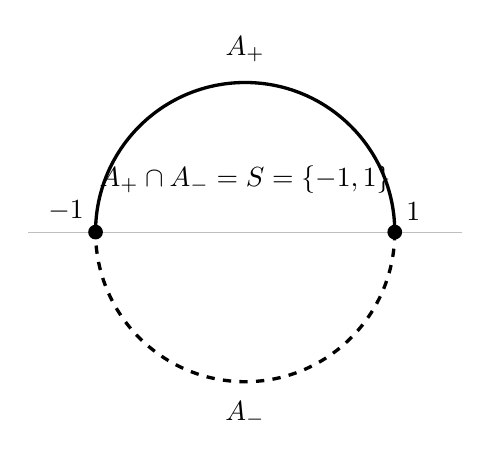
\begin{tikzpicture}[scale=1.9]
  % upper semicircle: solid carrier A_+
  \draw[very thick] (1,0) arc[start angle=0, end angle=180, radius=1];
  \node at (0,1.22) {$A_+$};
  % lower semicircle: dashed carrier A_-
  \draw[very thick, dashed] (1,0) arc[start angle=0, end angle=-180, radius=1];
  \node at (0,-1.22) {$A_-$};
  % faint horizontal axis for orientation
  \draw[gray!50] (-1.45,0) -- (1.45,0);
  % the package points
  \fill (-1,0) circle (1.4pt);
  \node[above left=1pt] at (-1,0) {$-1$};
  \fill (1,0) circle (1.4pt);
  \node[above right=1pt] at (1,0) {$1$};
  % annotation
  \node at (0,0.35) {$A_+\cap A_-=S=\{-1,1\}$};
\end{tikzpicture}
\caption{Two minimal carriers for the package $S=\{-1,1\}$: the upper
semicircle $A_+$ (solid) and the lower semicircle $A_-$ (dashed). Each is an
arc, hence a compact connected full continuum containing $S$, and they meet
only in the package points. A least carrier would be contained in their
intersection $S$, which is disconnected; hence no least carrier exists
(Theorem~\ref{thm:no-least}).}
\label{fig:no-least}
\end{figure}

\subsection{An analytic protected-access collision}\label{subsec:B-collision}

Theorem~\ref{thm:no-least} rules out selecting the carrier by minimization.
The remaining naive rule is completion: accept an arbitrary proposed carrier
and then absorb, monotonically, whatever excess the dynamics pulls back onto
it. The manuscript's Section~6.4 shows that this rule fails as well, and
fails in the most favorable analytic circumstances imaginable: a single
conformal, critical-value-free, degree-one branch of the quadratic map,
acting on an interval. The absorption step erases a protected prime-end
access, and monotonicity then propagates the erasure forever.

We reproduce the analytic setup exactly. Let
\[
f(z)=z^{2},\qquad I=[1,2],\qquad m=\tfrac32,
\]
and let
\begin{equation}\label{eq:B-Q}
Q=\Bigl\{\,z:\bigl|z-\tfrac32\bigr|\le\tfrac12,\ \operatorname{Im}z\ge 0\,\Bigr\}
\end{equation}
be the closed upper half-disk of radius $\tfrac12$ centered at $m$. Set
\[
U^{-}=\bigl\{z:\bigl|z-\tfrac32\bigr|<1\bigr\},
\qquad
U^{+}=f(U^{-}).
\]
The disk $U^{-}$ lies in the half-plane $\operatorname{Re}z>\tfrac12$. Two
consequences follow. First, $0\notin U^{-}$, so $f'(z)=2z\ne 0$ on $U^{-}$
and the critical point of $f$ is outside the domain; since $f(z)=f(w)$ forces
$w=\pm z$, and $U^{-}$ is disjoint from its antipode
$-U^{-}\subset\{\operatorname{Re}z<-\tfrac12\}$, the restriction
\begin{equation}\label{eq:B-branch}
F=f|_{U^{-}}:U^{-}\longrightarrow U^{+}
\end{equation}
is injective, hence a conformal homeomorphism onto $U^{+}$. Second, the
critical value $0=f(0)$ is not in $U^{+}$, so the branch is
critical-value-free. Take
\begin{equation}\label{eq:B-stages}
T_0=I,\qquad T_0'=Q,\qquad T_1=f(I)=[1,4],\qquad T_1'=f(Q).
\end{equation}
Within this branch the stage-$0$ data are the pullbacks of the stage-$1$
data:
\begin{equation}\label{eq:B-pullback}
T_0'=F^{-1}(T_1'),\qquad T_0=F^{-1}(T_1).
\end{equation}
Thus $T_0=I$ is the proposed carrier at stage $0$, and $T_0'=Q$ is the actual
pulled carrier: the completion rule under scrutiny would replace $T_0$ by an
enlargement absorbing the difference. Two pieces of terminology from the
manuscript's completion formalism are needed, and we define them at first
use. The \emph{pulled excess} at stage $0$ is the difference
$X_0=T_0'\setminus T_0$ between the pulled carrier and the proposed carrier.
The \emph{attachment trace} of the excess on the proposed carrier is
\begin{equation}\label{eq:B-trace}
\tau_{T_0}(X_0):=\overline{X_0}^{\,T_0'}\cap T_0,
\end{equation}
where $\overline{X_0}^{\,T_0'}$ denotes the closure of $X_0$ taken in the
actual pulled carrier $T_0'$: the trace records where the excess attaches to
the proposed carrier after closure, not where it meets it as a set.

\begin{proposition}[Quadratic protected-access collision; manuscript Proposition 6.15]\label{prop:access-collision}
In the setup \eqref{eq:B-Q}--\eqref{eq:B-pullback}, the pulled excess has the
single component
\[
X_0=Q\setminus I
\]
with attachment trace
\[
\tau_{T_0}(X_0)=\overline{X_0}^{\,T_0'}\cap T_0=I .
\]
The closure is taken in the actual pulled carrier $T_0'$; in particular, the
trace is not $X_0\cap T_0$, which is empty by the definition of the excess.
The complete one-stage itinerary of the excess is
\[
X_0\longmapsto f(X_0),
\]
through the conformal right-hand branch $F$, with no critical encounter.
Let $p_0^{+}(m)$ denote the upper landing access to $I$ at $m$, represented
by
\[
a_0(t)=m+it,\qquad 0<t\le\tfrac14.
\]
Every compact enlargement $H_0\Subset U^{-}$ with
$I\cup X_0\subset H_0$ erases this access.  Its image enlargement
$F(H_0)$ likewise erases the transported access
$F_*p_0^{+}(m)$, by which we mean the landing access represented by
$F\circ a_0$.
\end{proposition}

\begin{proof}
\emph{The excess and its trace.}
A point of $Q$ lies in $I=[1,2]$ exactly when it is real, so
\[
X_0=Q\setminus I
=\Bigl\{\,z:\bigl|z-\tfrac32\bigr|\le\tfrac12,\ \operatorname{Im}z>0\,\Bigr\}
\]
is the relative upper half-disk with its real diameter removed. It is the
intersection of the closed disk of radius $\tfrac12$ about $m$ with the open
upper half-plane, hence convex, hence connected: the excess has a single
component. Its closure in $\C$ is the entire closed half-disk
$Q$: every $x\in(1,2)$ is the limit of $x+it\in X_0$ as
$t\downarrow0$, while the endpoints are approached, for
$0<\varepsilon\le\tfrac12$, by
$1+\varepsilon+i\varepsilon$ and
$2-\varepsilon+i\varepsilon$, respectively.  As $Q=T_0'$, the closure of
$X_0$ in $T_0'$ is all of $Q$,
and therefore
\[
\tau_{T_0}(X_0)=\overline{X_0}^{\,T_0'}\cap T_0=Q\cap I=I:
\]
the excess attaches to the proposed carrier along the entire interval, even
though $X_0\cap T_0=\varnothing$ by construction. This is the reason the
completion formalism must work with attachment traces rather than
intersections: the naive intersection sees nothing, while the closure sees an
attachment along all of $I$.

\emph{The itinerary.}
Since $0\notin U^{-}$, we have $F'(z)=2z\ne 0$ throughout $U^{-}$, and the
selected branch avoids the critical value $0\notin U^{+}$. The itinerary of
the excess therefore consists of the single right-sheet, degree-one step
$X_0\mapsto f(X_0)$ with no critical encounter.
There is no hidden multivalence, folding, or critical intrusion anywhere in
the example.

\emph{Erasure of the protected access.}
The access $p_0^{+}(m)$ is the access to $I$ at the interior point $m$ from
the upper side, represented by $a_0$, which lies in
$U^{-}\setminus I$ and lands at $m$.  Let
$H_0\Subset U^{-}$ be compact and contain $X_0\cup I=Q$.  The set $Q$ contains an
upper relative half-neighborhood of $m$: the set
\[
\Bigl\{\,z:\bigl|z-\tfrac32\bigr|<\tfrac12,\ \operatorname{Im}z\ge 0\,\Bigr\}
\subset Q
\]
is a neighborhood of $m$ in the closed upper half-plane. Consequently, any
curve in $U^{-}$ landing at $m$ from the upper side---that is, eventually
in the upper component of a sufficiently small disk about $m$ with $I$
removed---eventually lies in this half-neighborhood, hence in $Q\subset H_0$.
No curve in the complement $U^{-}\setminus H_0$ can therefore land at $m$ from the upper
side: the access $p_0^{+}(m)$ no longer exists as an access from the
complement of $H_0$.  Any further enlargement still contains $Q$ and
cannot restore that access.

\emph{Transport to stage $1$.}
The branch $F$ of \eqref{eq:B-branch} is a conformal homeomorphism of
$U^{-}$ onto $U^{+}$ carrying $I$ to $T_1=[1,4]$, $Q$ to $T_1'$, $X_0$ to the
stage-$1$ excess $T_1'\setminus T_1$, and the representing curve $m+it$ to a
curve in $U^{+}\setminus T_1$ landing at $f(m)=\tfrac94$ from the
$F$-selected side.  The compact image $F(H_0)$ contains
$F(Q)=T_1'$.  A homeomorphism of the localization carries complement
curves to complement curves, so the same argument applied to these image data
erases the transported access $F_{*}p_0^{+}(m)$ at stage $1$. Conformality
thus transports the identical conclusion to stage $1$, as claimed.
\end{proof}

\begin{figure}[ht]
\centering
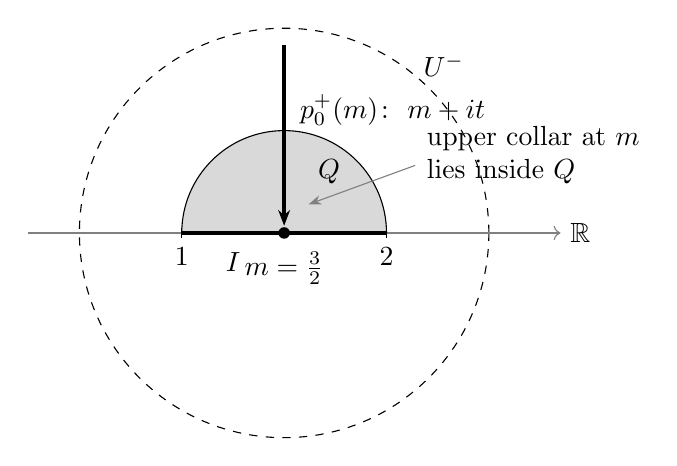
\begin{tikzpicture}[scale=2.6]
  % localization disk U^- (dashed)
  \draw[dashed] (1.5,0) circle[radius=1];
  \node at (2.28,0.82) {$U^{-}$};
  % real axis
  \draw[->,gray] (0.25,0) -- (2.85,0) node[right,black] {$\mathbb{R}$};
  % excess half-disk Q (shaded)
  \fill[gray!30] (2,0) arc[start angle=0, end angle=180, radius=0.5] -- cycle;
  \draw (2,0) arc[start angle=0, end angle=180, radius=0.5];
  \node at (1.72,0.3) {$Q$};
  % proposed carrier I = [1,2]
  \draw[very thick] (1,0) -- (2,0);
  \draw (1,0.025) -- (1,-0.025) node[below] {$1$};
  \draw (2,0.025) -- (2,-0.025) node[below] {$2$};
  \node[below] at (1.25,-0.05) {$I$};
  % marked point m
  \fill (1.5,0) circle (0.8pt);
  \node[below] at (1.5,-0.045) {$m=\tfrac32$};
  % protected access arrow from above, along m + it
  \draw[-{Stealth[length=2mm]},very thick] (1.5,0.92) -- (1.5,0.035);
  \node[right] at (1.53,0.6) {$p_0^{+}(m)\colon\ m+it$};
  % annotation: the collar at m is inside Q
  \node[align=left,right] at (2.15,0.38) {upper collar at $m$\\ lies inside $Q$};
  \draw[-{Stealth[length=1.6mm]},gray] (2.14,0.33) -- (1.62,0.14);
\end{tikzpicture}
\caption{The quadratic protected-access collision
(Proposition~\ref{prop:access-collision}). The proposed carrier is the
interval $I=[1,2]$ (thick); the pulled carrier is the closed upper half-disk
$Q$ (shaded) of radius $\tfrac12$ about $m=\tfrac32$, inside the localization
disk $U^{-}$ (dashed) on which $f(z)=z^{2}$ restricts to a conformal
homeomorphism. The protected upper access $p_0^{+}(m)$, represented by the
vertical segment $m+it$, must traverse $Q$: absorbing the excess
$X_0=Q\setminus I$ forces the carrier to contain the entire upper collar at
$m$ and erases the access.}
\label{fig:access-collision}
\end{figure}

\subsection{What the obstructions force}\label{subsec:B-moral}

The two obstructions are complementary and together close off every naive
route. Theorem~\ref{thm:no-least} shows that the carrier cannot be
\emph{selected} canonically: there is no least connected full hull, even for
two points with identity dynamics.  Minimal carriers may exist, as the two
semicircles in the proof show, but they need not be unique and neither is
least; thus ``the minimal carrier'' does not specify an object.
Proposition~\ref{prop:access-collision} shows that the carrier cannot be
\emph{completed} blindly either: the very first monotone absorption of a
pulled excess can erase a protected prime-end access, and monotonicity then
makes the loss irreversible at every later stage of the enlargement, as well
as at the conformally transported stage.

The second obstruction is the sharper of the two, because of what it does
\emph{not} involve. In the manuscript's collision bookkeeping \cite{MWman},
which records sheet mergers, critical intrusions, obstacle collisions, access
identifications, and localization escapes in the order
$(\chi_{\mathrm{sheet}},\chi_{\mathrm{crit}},\chi_{\mathrm{obs}},
\chi_{\mathrm{access}},\chi_{\mathrm{loc}})$, the collision tuple of the
completed enlargement in this example is
\[
\bigl(\varnothing,\ \varnothing,\ \varnothing,\
\{p_0^{+}(m),\,F_{*}p_0^{+}(m)\},\ \varnothing\bigr):
\]
every coordinate vanishes except the access coordinate. The
branch is conformal, degree one, and critical-value-free; there is no sheet
merger, no obstacle, and no localization escape. Consequently no amount of
critical-point bookkeeping---however carefully one tracks critical points,
critical values, or degrees---can detect, let alone excuse, the collision.
Access protection is invisible to critical data and must be carried as
explicit data of its own, with its own survival theorem.

This is exactly what the remainder of the paper provides. The certificate
formalism of Section~\ref{sec:certificates} records the protected accesses as
prime-end crosscut chains \cite{Pom92} with pairwise disjoint relative
terminal collar tails, together with free-port arcs carrying singleton attachment traces
and a ribbon tree with declared sides; Theorem~\ref{thm:realization} then
realizes any such certificate by an actual compact connected full carrier in
which every protected chain survives with unchanged cyclic order. The
selection ambiguity of Theorem~\ref{thm:no-least} is resolved not by
minimization but by the certificate itself: the connector system, its access
class, and its routing are supplied as data, and the exact free-component
criterion of Section~\ref{sec:criterion} determines precisely when such data
can be supplied at all.
% ---- end B:obstructions ----

% ---- begin A:comparison ----
% Cluster A: comparison with standard continuum-hull constructions
% Review-required new expository material; promotes no manuscript claim.
% Body-only LaTeX; preamble macros, cite keys, and cross-cluster labels per CONVENTIONS.md.

\section{Comparison with standard continuum-hull constructions}
\label{sec:comparison}

The certificate formalism developed from Section~\ref{sec:certificates}
onward is offered as a replacement for a family of standard constructions,
and it is fair to ask what, exactly, is being replaced and why.  This
section compares the framework with five natural comparison points:
least or minimal connected full hulls; monotone
absorption of pulled excess; regulated and Hubbard trees in uniformized or
locally connected coordinates; Moore decompositions and monotone
quotients; and the lamination-lift candidate of the source manuscript.
The two obstructions of Section~\ref{sec:obstructions} already dispose of
the first two; the remaining three fail for structural reasons that are
worth stating precisely, because they explain several design decisions of
the certificate formalism that would otherwise look pedantic.  Throughout,
the comparison is with respect to the task fixed in the introduction:
join finitely many pairwise disjoint full atoms inside a Jordan
localization, avoid a frozen forbidden set, and \emph{preserve designated
prime-end accesses together with their cyclic order}.  Constructions that
solve a different problem well are not thereby criticized; the claim is
only that none of the constructions, in the forms reviewed here, records
all of these requirements simultaneously, and that the last of them ---
the lamination lift --- is an open candidate, not a construction.

\subsection{Least and minimal connected full hulls}
\label{subsec:A-comp-least}

The most tempting rule is extremal: ``take the least connected full hull
of the required package.''  Theorem~\ref{thm:no-least} (manuscript
Theorem~6.12) shows the rule names no object, already for the two-point
package $S=\{-1,1\}$ with identity dynamics and no obstacles: the upper
and lower semicircles are carriers meeting exactly in $S$, so a least
carrier would be contained in their disconnected intersection.  The
failure is specific to \emph{leastness}: minimal carriers exist in
abundance --- every arc from $-1$ to $1$ is one --- and form a large
antichain.  An extremal selection principle therefore cannot even break
the tie between the two semicircles, and the tie is not innocent: the two
choices pass on opposite sides of the origin, and in any configuration
with obstacles or relative protected collar tails that choice of side is visible to
every later routing step.  The source manuscript sharpens the point
dynamically \cite[Proposition~6.11]{MWman}: a package, full connected
carriers, critical-value-free degree-one selected-carrier dynamics, and
identical coarse orbit labels are realized simultaneously by an interval
and by a triod, and attachment-freeness holds in only one of the two
models, so no data of the listed kinds can select between them.

The connected-hull descriptions in the renormalization
literature are not at fault here, and the comparison should not be read
as a criticism of them.  Dudko's roadmap describes virtual Julia sets as
connected hulls of Cantor families of small Julia sets carrying a finite
part of the critical orbit \cite{Dud25}; that description specifies
\emph{which} continua a carrier must contain, and it does not purport to
specify \emph{how} they are joined.  Theorem~\ref{thm:no-least} shows
that the routing is genuinely additional data --- in the manuscript's
words, a regulated connector system, together with its access or isotopy
class and a forward-coherence proof, is additional data \cite{MWman} ---
and the certificate of Definition~\ref{def:certificate} is exactly a
format for that data, with Theorem~\ref{thm:free-component} deciding when
the format can be filled in at all.

\subsection{Monotone absorption of pulled excess}
\label{subsec:A-comp-absorption}

The second rule is completion: accept any proposed carrier and absorb,
monotonically, whatever excess the dynamics pulls back onto it, until the
process stabilizes.  Unlike the least hull, this rule is well defined:
the manuscript proves that the finite inflationary completion operator
stabilizes at a least fixed point, unique and conjugation-equivariant
\cite[Theorem~6.14]{MWman}.  The defect is not existence but what
completion destroys.  Proposition~\ref{prop:access-collision} (manuscript
Proposition~6.15) exhibits a conformal, critical-value-free, degree-one
branch of $z\mapsto z^2$ in which the very first absorption of pulled
excess --- the relative upper half-disk attaching to the interval along
its entire length --- erases a protected prime-end access and its
conformally transported copy.  Monotonicity, the rule's defining virtue,
is precisely what makes the loss permanent: enlargement can only add
points, and no addition restores a complement access through a set
already absorbed.  Moreover, every coordinate of the manuscript's
collision bookkeeping except the access coordinate vanishes in this
example, so no amount of critical-value, degree, or sheet bookkeeping
detects the erasure (Section~\ref{subsec:B-moral}).

The certificate formalism keeps monotone completion but reverses the
order of commitments.  The relative protected collar tails are frozen into the
inventory $Q$ \emph{before} any absorption is contemplated; a proposed
absorption that would enter such a tail is not a step of a completion
but a named violation, and the persistence clause of
Theorem~\ref{thm:free-component}, together with the audit of
Theorem~\ref{thm:audit}, converts each such violation into a certificate
--- a merger, a port loss, a separation --- that survives every further
monotone enlargement.  Absorption remains available for everything
unprotected; what changes is that ``protected'' is a constraint checked
by the plane, not an intention held by the author.

\subsection[Regulated and Hubbard trees]
{Regulated trees in uniformized coordinates and Hubbard trees}
\label{subsec:A-comp-trees}

For a postcritically finite polynomial $P$ with connected filled Julia
set, the classical Hubbard tree is the regulated hull in $K(P)$ of the
finite union of the forward critical orbits \cite{DHOrsay}.  Arbitrary finite
invariant sets, or local connectivity alone, do not define the classical
Hubbard tree.  The construction uses regulated arcs, uniformized
coordinates, and canonical internal arcs.  Local connectivity gives a
continuous extension of the exterior Riemann map to the boundary; that
extension is a homeomorphism only when the boundary is a Jordan curve
\cite{DHOrsay,Pom92}.  Kahn--Lyubich impose finite-decoration combinatorics
and prove a~priori bounds for that class, using puzzle pieces, rays, and
equipotentials in the construction \cite{KL08}.

None of these steps is guaranteed by the standing hypotheses of the
present paper.  The atoms are arbitrary full continua; no Riemann map is
asserted to extend, no external or internal ray is asserted to land, and
regulated arcs need not exist.  This is not a hypothetical worry but the
operating regime of the intended applications, in which local
connectivity of the relevant continua is exactly what is not known.  The
closest publicly available construction is instructive as a boundary
marker.  In its stated primitive-renormalization setting, the preprint of
Kahn--Kapiamba--Lyubich uses a rational-lamination quotient, a locally
connected combinatorial model, and the associated natural projection
\cite[\S\S2.5--2.6]{KKL26}.  This is not a general construction for
arbitrary full continua.  As the source manuscript's own boundary records
\cite{MWman}, the preprint is a positive control in its
primitive-renormalization category, not a theorem for the arbitrary
packages contemplated here.  The framework of this paper is
calibrated to the complementary regime: Theorem~\ref{thm:realization}(6)
uses no local connectivity of any atom, the tree of the certificate is
produced by the exact criterion of Theorem~\ref{thm:free-component} from
planar data alone, and no canonicity of the spanning tree is claimed
anywhere --- the tree is data, chosen in a free component whose existence
is the actual content.  What is lost relative to the Hubbard-tree regime
is canonicity; what is gained is existence without a locally connected
model whenever the exact free-component criterion holds.

\subsection{Moore decompositions and monotone quotients}
\label{subsec:A-comp-moore}

A third classical route collapses instead of routing.  Moore's theorem
states that if $\mathcal G$ is an upper-semicontinuous decomposition of
$S^2$ into nonseparating continua and the quotient has more than one
point, then $S^2/\mathcal G$ is homeomorphic to $S^2$ \cite{Moo25}.
One is therefore tempted to collapse every atom (or every
completed packet) to a point, join the finitely many image points by
arcs in the quotient sphere --- where the joining problem is trivial ---
and pull the picture back.  For the connection problem \emph{without}
protected data this can be a serviceable device and is one standard
mechanism for passing to a simpler quotient model.

For the access-preserving problem the unmarked quotient is not, by itself,
a certificate.  Collapsing an atom sends all of its points to one quotient
point, and neither that point nor a tree incident to it records which named
prime ends, selected sides, or relative collar tails are to be protected.
Crosscuts in the complement can have quotient images, and in favorable
decompositions distinct approaches may still be recoverable; the point is
that Moore's theorem alone supplies none of the required marking or
survival conclusions.  Those data would have to be transported separately.

Likewise, the preimage of an arc under a continuous monotone quotient is
a continuum, but generally a saturated one.  It does not automatically
have singleton attachment traces, retain selected prime-end accesses, or
preserve marking data; a fiber can contain more attachment material or
meet a forbidden collar.  Thus a Moore quotient may support a construction only
after it is augmented by the same access and incidence data that the
certificate formalism records explicitly.  The present realization works
in the original plane, carries protected accesses as crosscut chains with
selected sides, and attaches its connector at declared free ports with
singleton traces (Theorem~\ref{thm:realization}(2)).

\subsection{The lamination-lift candidate}
\label{subsec:A-comp-lamination}

The most serious competitor is the manuscript's own candidate, recorded
in its Section~10.3 \cite{MWman}, and the comparison must be exact:
the candidate is presented there, and here, as a candidate only.
Suppose, following the non-locally-connected construction of
Kahn--Kapiamba--Lyubich \cite{KKL26}, that an ambient carrier admits a
monotone semiconjugacy
\[
\pi\colon K\longrightarrow K_{\mathrm{com}}
\]
onto a locally connected combinatorial model, together with a
forward-coherent regulated tree $T_{\mathrm{com}}\subset K_{\mathrm{com}}$
containing the prescribed finite marked set.  The canonical candidate connector is
\begin{equation}\label{eq:A-lam}
H_{\mathrm{lam}}\;=\;\Fill\bigl(\pi^{-1}(T_{\mathrm{com}})\bigr),
\end{equation}
equation~(9.3) of \cite{MWman}.  Part of what is wanted is genuinely
true, by soft arguments: a monotone preimage of a compact connected set
is compact and connected, so \eqref{eq:A-lam} is a full continuum
containing the preimage of the prescribed marked set; the semiconjugacy provides forward
coherence before fullification; and fullification preserves genuine
polynomial forward invariance.

The missing assertion is not connectedness.  Measured against the
certificate clauses, two failure channels are named in the manuscript,
and both remain unresolved.  First, a projection fiber
$\pi^{-1}(x)$ over a point of the tree, or a component added by
fullification, may enter a protected collar otherwise than at a declared
free singleton port; this is the erasure mechanism of
Proposition~\ref{prop:access-collision} wearing different clothes, and
it is instructive that the manuscript rejects the upper-half-disk
collision at exactly this clause, the excess occupying the protected
upper collar with an interval attachment trace \cite{MWman}.  Second, a
disconnected stage package may still split across iterated pullback
components, so that containing the prescribed marked set does not yet realize
the complete package routing.  The manuscript collects the clauses a
proof would have to establish --- authorized localization and complete
frozen inventory, collar avoidance except at declared free singleton
ports, realization of every package component and route, obstacle
handling inside the localization, complete access marking, and an
incidence bound or compression --- as its Open Problem~10.6 (Virtual
Protected Routing Certificate).  That problem is open, and nothing in
this paper resolves any part of it; consistently with the manuscript's
Warning~10.59, the candidate \eqref{eq:A-lam} is discussed here only to
locate it on the map.

What this paper contributes to the candidate is the deciding instrument,
not a verdict.  For any frozen inventory that a future argument
supplies, Theorem~\ref{thm:free-component} decides certificate existence
exactly; Theorems~\ref{thm:common-domain} and~\ref{thm:audit} and
Proposition~\ref{prop:cellwise} make the decision checkable packet by
packet; and the two failure channels above fall under the typed,
monotone-persistent defect certificates of Section~\ref{sec:audit} ---
a fiber in a collar is a port-loss or merger defect, a split package is
a separation in the sense of the persistence clause of
Theorem~\ref{thm:free-component}.  Whether the candidate passes the test
is precisely what is open.

\subsection{Summary}
\label{subsec:A-comp-summary}

Table~\ref{tab:A-comparison} compresses the comparison.  The pattern is
uniform: each standard construction either fails to exist (the least
hull), can destroy the protected data (absorption), does not by itself
record those data (Moore quotients),
requires the hypothesis whose absence is the whole difficulty (regulated
and Hubbard trees), or is an explicitly open candidate (the lamination
lift).  The certificate framework renounces canonicity --- the connector
is data, not an invariant --- and in exchange obtains, for arbitrary
full atoms and with no local connectivity of the atoms: realization of every
supplied certificate with
access survival and cyclic-order preservation
(Theorem~\ref{thm:realization}); an exact existence criterion on frozen
data (Theorem~\ref{thm:free-component}); checkable sufficient tests
(Theorem~\ref{thm:common-domain}, Proposition~\ref{prop:cellwise});
order-independent completion with a three-clause audit
(Theorem~\ref{thm:audit}); and failure certificates that persist under
monotone enlargement.  The effect is to convert ``choose a hull,''
an instruction that Theorem~\ref{thm:no-least} shows to be ill posed and
Proposition~\ref{prop:access-collision} shows to be destructive, into a
checkable planar test with a stable answer in both directions.  This is
the precise sense in which the contribution of the paper is proof
technology: no new theorem of classical planar topology is claimed, and
every statement about the open constructions touched on above ---
virtual carriers, lamination lifts, and their dynamical certificates ---
remains exactly as open here as in the source manuscript.

\begin{table}[H]
\centering
\small
\begin{tabularx}{\textwidth}{@{}P{0.25\textwidth}P{0.22\textwidth}P{0.22\textwidth}Y@{}}
\toprule
Construction & Existence & Access guarantee & Failure witness\\
\midrule
least connected full hull & no (Thm.~\ref{thm:no-least}) & --- & ---\\
monotone absorption & least fixed point \cite{MWman} &
  erasable (Prop.~\ref{prop:access-collision}) & post hoc only\\
regulated/Hubbard tree & needs locally connected model \cite{DH85,KKL26} &
  native category only & ---\\
Moore monotone quotient & specified nontrivial u.s.c.\ decomposition
  into nonseparating continua \cite{Moo25} &
  markings not automatic & ---\\
lamination lift \eqref{eq:A-lam} & candidate \cite{MWman} & open & open\\
protected certificate & exact criterion (Thm.~\ref{thm:free-component}) &
  preserved (Thm.~\ref{thm:realization}) &
  persistent (Thm.~\ref{thm:audit})\\
\bottomrule
\end{tabularx}
\caption{The five standard constructions against the certificate
framework, measured on the access-preserving connection task.  ``Existence''
asks whether the construction produces a well-defined carrier
for arbitrary pairwise disjoint full atoms in a Jordan localization;
``access guarantee'' asks whether designated prime-end data survive
with their cyclic order; ``failure witness'' asks whether a negative
outcome is witnessed by a certificate that persists under monotone
enlargement.  The lamination-lift row records candidacy, not failure:
its clauses are the manuscript's open problem, and no verdict is implied
in either direction.}
\label{tab:A-comparison}
\end{table}
% ---- end A:comparison ----

% ---- begin C:certificates ----
% Cluster C: certificates and realization (manuscript §10.2)
% Body-only LaTeX; preamble macros and theorem environments per CONVENTIONS.md.

\section{Protected ribbon-routing certificates and realization}
\label{sec:certificates}

The two obstructions of the preceding section calibrate what a realization
theorem can promise.  Theorem~\ref{thm:no-least} shows that even the
two-point package with identity dynamics and no obstacles admits no least
compact connected full carrier, so no canonical minimal choice is available
and a connector must be \emph{supplied}, not selected by an extremal
principle.  Proposition~\ref{prop:access-collision} shows that a compact
enlargement absorbing the pulled excess can permanently erase a protected prime-end
access even along a conformal, critical-value-free branch: once a set
occupying a protected side has been absorbed, no further monotone
enlargement restores an access through it.  Together these force the shape
of the present section.  The connector data must be recorded \emph{in
advance}, as an explicit finite certificate that names every protected
access, reserves a collar around each one, and routes the connecting tree
through the reserved-free region.  The theorem then owed to the reader is
purely topological: every such certificate is realized by a compact
connected full carrier, the protected accesses survive as prime ends of the
enlarged complement, distinct accesses stay distinct, their cyclic order is
unchanged, and the two regular-neighborhood side-readings of each connector
edge appear in the boundary order dictated by the ribbon structure of the
tree.  This is the
content of Theorem~\ref{thm:realization} below.  The section closes with
the naturality of the construction under univalent changes of the Jordan
localization (Proposition~\ref{prop:naturality}).  The question of when a
certificate \emph{exists} is deferred to
Section~\ref{sec:criterion}, where it receives an exact answer.

\subsection*{Setup}
Throughout this section $U\subset\C$ is a Jordan disk, that is, a bounded
simply connected domain whose boundary is a Jordan curve.  A
\emph{continuum} is a nonempty compact connected subset of $\C$; a
continuum $K$ is \emph{full} if $\C\setminus K$ is connected, equivalently
if $\Chat\setminus K$ is a simply connected domain containing $\infty$.
Following the source manuscript \cite{MWman}, the full continua to be
joined are called \emph{atoms}.  Fix $s\ge1$, and let
\[
A_1,\dots,A_s\Subset U
\]
be pairwise disjoint atoms, and let
\[
Z\Subset U\setminus\bigcup_{i}A_i
\]
be the compact frozen forbidden set.  It bundles every non-collar
obstacle, critical-value exclusion, and localization exclusion.  Nothing
in this section uses any dynamical structure
on the $A_i$ or on $Z$; the data are purely planar.

For each nondegenerate atom $A_i$, the domain
$\Omega_i=\Chat\setminus A_i$ is simply connected and the prime-end
formalism of Section~\ref{subsec:A-primeends} applies \cite{Pom92}.
Protected chains are permitted only at nondegenerate atoms; a degenerate
atom may still carry a free port and participate in the carrier, but its
protected-label set is empty.  All chains below are \emph{null chains} in the
sense of
\eqref{eq:A-null-chain}:
\[
 \overline{D_{n+1}}\setminus A_i\subset D_n,
 \qquad
 \operatorname{diam}_{\mathrm{sph}}(\gamma_n)\longrightarrow0.
\]
The record of a chain contains, for every $n$, the declaration of which
side $D_n$ of $\gamma_n$ is selected.  It is exactly this declaration that
the certificates below protect.

For every protected access to a nondegenerate $A_i$, indexed by a finite
set of labels $a$ specifying pairwise distinct prime ends at that fixed
atom, choose a prime-end crosscut chain
\[
\Gamma_{i,a}=(\gamma_{i,a,n},\,D_{i,a,n})_{n\ge1}
\]
of $\Chat\setminus A_i$.  The chains are truncated, that is, an initial
segment of each is discarded and the indices shifted, so that the terminal
\emph{relative collar tails}
\[
\overline{D_{i,a,1}}\setminus A_i
\]
are pairwise disjoint, lie in $U$, and miss $Z$ and the other atoms.  For
each fixed atom, Hausdorff separation in its prime-end closed disk gives
pairwise disjoint sufficiently deep prime-end neighborhoods.  Across
different atoms, choose pairwise disjoint Euclidean neighborhoods
$V_i\Subset U$ of the compact sets $A_i$, all disjoint from $Z$.
Because the nested compact sets $\overline{D_{i,a,n}}$ decrease to their
impressions in $A_i$, sufficiently deep members lie in $V_i$.  A common
finite truncation therefore has all the stated properties.  Their closures are allowed
to meet inside a common atom, so overlapping prime-end impressions are not
excluded.  The set $D_{i,a,1}$ is called the (terminal, or first)
\emph{protected collar} of the access $(i,a)$; every deeper selected domain
$D_{i,a,n}$ lies inside it.  Figure~\ref{fig:collar} shows a single atom,
one protected chain, its nested selected domains, and its collar.

\begin{figure}[htbp]
\centering
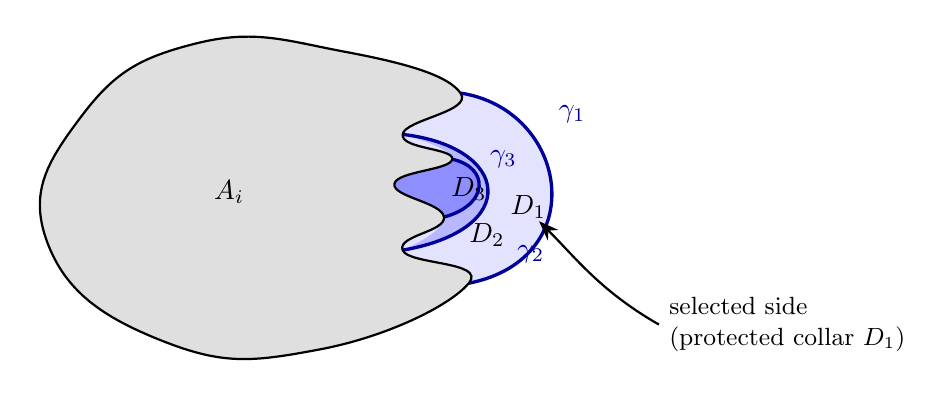
\begin{tikzpicture}[scale=1.05, line join=round]
% ---- selected domains D_1 > D_2 > D_3 (filled before the atom, which
% ---- is drawn on top and cleans up the shared boundary) ----
% D_1: region between crosscut gamma_1 and the oscillating boundary edge
\fill[blue!55, opacity=0.20]
  (0.2,1.1) .. controls (1.5,0.9) and (1.8,-0.9) .. (0.3,-1.2)
  plot [smooth, tension=0.8] coordinates
    {(0.3,-1.2) (-0.5,-0.8) (0.0,-0.4) (-0.6,0.0) (0.1,0.3) (-0.5,0.6) (0.2,1.1)};
% D_2
\fill[blue!55, opacity=0.38]
  (-0.5,0.6) .. controls (0.8,0.45) and (0.95,-0.55) .. (-0.5,-0.8)
  plot [smooth, tension=0.8] coordinates
    {(-0.5,-0.8) (0.0,-0.4) (-0.6,0.0) (0.1,0.3) (-0.5,0.6)};
% D_3
\fill[blue!55, opacity=0.60]
  (0.1,0.3) .. controls (0.55,0.2) and (0.55,-0.25) .. (0.0,-0.4)
  plot [smooth, tension=0.8] coordinates
    {(0.0,-0.4) (-0.6,0.0) (0.1,0.3)};
% ---- crosscuts ----
\draw[very thick, blue!60!black]
  (0.2,1.1) .. controls (1.5,0.9) and (1.8,-0.9) .. (0.3,-1.2);
\draw[very thick, blue!60!black]
  (-0.5,0.6) .. controls (0.8,0.45) and (0.95,-0.55) .. (-0.5,-0.8);
\draw[very thick, blue!60!black]
  (0.1,0.3) .. controls (0.55,0.2) and (0.55,-0.25) .. (0.0,-0.4);
% ---- the atom: an irregular, non-locally-connected-looking blob ----
\fill[gray!25]
  plot [smooth cycle, tension=0.8] coordinates
    {(0.2,1.1) (-1.2,1.6) (-3.0,1.7) (-4.4,0.8) (-4.8,-0.7) (-3.4,-1.9)
     (-1.5,-2.0) (0.3,-1.2) (-0.5,-0.8) (0.0,-0.4) (-0.6,0.0) (0.1,0.3)
     (-0.5,0.6)};
\draw[thick]
  plot [smooth cycle, tension=0.8] coordinates
    {(0.2,1.1) (-1.2,1.6) (-3.0,1.7) (-4.4,0.8) (-4.8,-0.7) (-3.4,-1.9)
     (-1.5,-2.0) (0.3,-1.2) (-0.5,-0.8) (0.0,-0.4) (-0.6,0.0) (0.1,0.3)
     (-0.5,0.6)};
% ---- labels ----
\node at (-2.6,-0.1) {$A_i$};
\node[blue!60!black] at (1.55,0.85) {$\gamma_1$};
\node[blue!60!black] at (1.05,-0.85) {$\gamma_2$};
\node[blue!60!black] at (0.72,0.30) {$\gamma_3$};
\node at (1.02,-0.28) {$D_1$};
\node at (0.52,-0.62) {$D_2$};
\node at (0.30,-0.06) {$D_3$};
% selected-side arrow
\draw[-{Stealth[length=2.5mm]}, thick]
  (2.6,-1.7) node[right, align=left, font=\small]
  {selected side\\ (protected collar $D_1$)}
  .. controls (1.9,-1.3) and (1.6,-0.9) .. (1.15,-0.45);
\end{tikzpicture}
\caption{A protected prime-end crosscut chain at a single atom $A_i$.  The
crosscuts $\gamma_1,\gamma_2,\gamma_3$ are pairwise disjoint arcs of
$\Chat\setminus A_i$ with endpoints on $\partial A_i$ and shrinking
diameters; the shaded regions are the nested selected sides
$D_1\supset D_2\supset D_3$, drawn with increasing opacity toward the
prime end.  The outermost selected domain $D_1$ is the protected collar of
the access: after truncation the relative collar tail
$\overline{D_1}\setminus A_i$ is disjoint from every other relative tail,
lies in $U$, and misses the
obstacle set $Z$ and the other atoms.  The boundary of the atom is drawn
deliberately oscillating: no local connectivity of $\partial A_i$ is
assumed anywhere in this section, and the access is carried entirely by
the chain, not by any landing curve.}
\label{fig:collar}
\end{figure}

\begin{definition}[Protected ribbon-routing certificate; manuscript
Definition 10.1]\label{def:certificate}
A \emph{protected ribbon-routing certificate} consists of the preceding
data---the Jordan disk $U$, the atoms $A_1,\dots,A_s$, the forbidden set
$Z$, and the truncated protected chains $\Gamma_{i,a}$---together with
pairwise disjoint Jordan embeddings
$\alpha_i\colon[0,1]\hookrightarrow U$, called \emph{free-port arcs},
satisfying
\[
\alpha_i\cap A_i=\{x_i\},\qquad
\alpha_i((0,1])\cap
\Bigl(Z\cup\bigcup_{j}A_j\cup
\bigcup_{j,a}(\overline{D_{j,a,1}}\setminus A_j)\Bigr)=\varnothing,
\]
where $x_i=\alpha_i(0)$, and an embedded finite tree $G\subset U$ joining
the outer port endpoints $\alpha_1(1),\dots,\alpha_s(1)$ while missing the
same protected and forbidden sets
$Z\cup\bigcup_jA_j\cup
\bigcup_{j,a}(\overline{D_{j,a,1}}\setminus A_j)$, subject to
\[
 G\cap\alpha_i=\{\alpha_i(1)\}\quad(1\le i\le s),
 \qquad
 G\cup\bigcup_i\alpha_i\ \text{an embedded finite plane tree}.
\]
As usual, a finite tree may be degenerate, consisting of one vertex and no
edges; this convention is used when $s=1$.
The planar cyclic order of
half-edges at every vertex of $G$ is retained as part of the certificate
(its \emph{ribbon structure}).  Every access read by a proof must be a
protected chain $\Gamma_{i,a}$; every connector-side reading must be a
declared side of this ribbon tree, interpreted through the boundary of a
thin regular neighborhood.
\end{definition}

Given a certificate $R$, define its \emph{carrier}
\begin{equation}\label{eq:C-HR}
H_R \;=\; G\cup\bigcup_i\alpha_i\cup\bigcup_iA_i .
\end{equation}
The finite plane tree
\[
T_R:=G\cup\bigcup_i\alpha_i
\]
is its \emph{connector tree}, and $T_R\cap A_i$ is the
\emph{connector attachment trace} at $A_i$.

Four reading notes.  First, the port arc $\alpha_i$ touches its atom at
the single \emph{free port} $x_i$, and its positive-parameter part avoids
every protected relative collar tail, including those based at the same
atom.  The abstract certificate does not require $x_i$ to avoid a protected
impression inside $A_i$; applications that need that stronger marking
condition impose it explicitly through the unprotected exposure locus of
Section~\ref{sec:audit}.  Second, ``joining the outer port
endpoints'' is read as part of the embeddedness of the certificate: the
tree $G$ meets each port arc $\alpha_i$ in exactly the point
$\alpha_i(1)$, so that $G\cup\bigcup_i\alpha_i$ is again an embedded
finite tree, with the port arcs attached as pendant edges.  This is the
configuration produced by the construction of
Section~\ref{sec:criterion}, where the routing tree is built in the
complement of the slit port arcs, and it is used in the proof of the
realization theorem below.  Third, the tree $G$ is a
combinatorial object with a planar enhancement: recording the cyclic order
of half-edges at each vertex fixes, up to isotopy, the two sides of every
edge, and it is these \emph{declared ribbon sides} that the realization
theorem reads, through thin regular neighborhoods, in a prescribed
boundary order.  No prime end associated with an individual tree edge is
asserted.
Fourth, the final sentence of the definition is a discipline on all later
arguments, not a property of the data: any subsequent proof that consults
an access of the carrier must consult a protected chain, and any proof that
consults a connector side must use a declared ribbon side rather than an
incidental feature of a particular embedding.  Figure~\ref{fig:certificate} shows a
certificate with three atoms.

\begin{figure}[htbp]
\centering
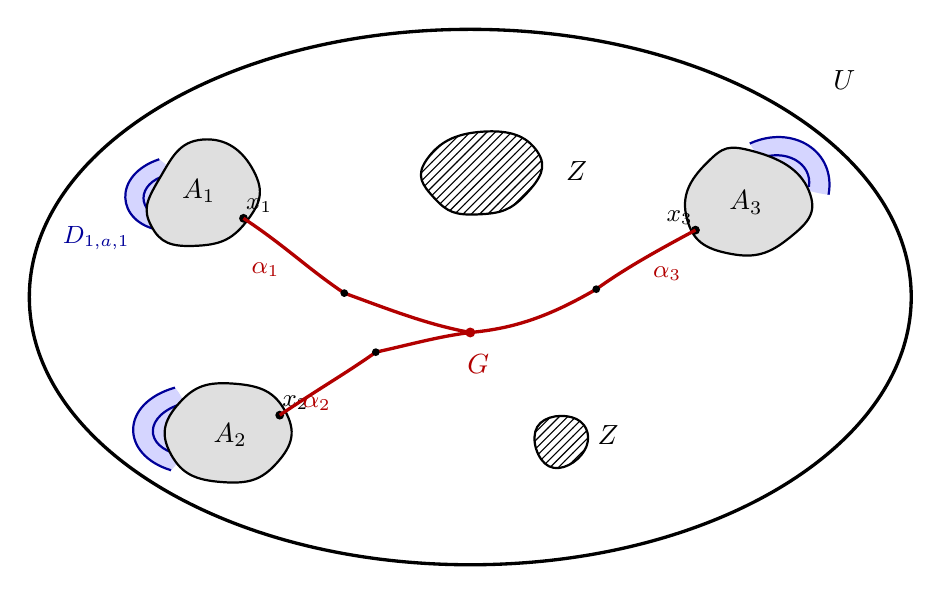
\begin{tikzpicture}[scale=1.0, line join=round]
% ---------- Jordan disk U ----------
\draw[very thick] (0,0) ellipse (5.6 and 3.4);
\node at (4.75,2.75) {$U$};
% ---------- obstacle set Z (hatched) ----------
\fill[pattern=north east lines]
  plot [smooth cycle, tension=0.9] coordinates
    {(0.1,1.05) (0.7,1.30) (0.85,1.85) (0.15,2.10) (-0.55,1.75) (-0.45,1.25)};
\draw[thick]
  plot [smooth cycle, tension=0.9] coordinates
    {(0.1,1.05) (0.7,1.30) (0.85,1.85) (0.15,2.10) (-0.55,1.75) (-0.45,1.25)};
\fill[pattern=north east lines]
  plot [smooth cycle, tension=0.9] coordinates
    {(1.0,-2.15) (1.45,-1.95) (1.35,-1.55) (0.85,-1.65)};
\draw[thick]
  plot [smooth cycle, tension=0.9] coordinates
    {(1.0,-2.15) (1.45,-1.95) (1.35,-1.55) (0.85,-1.65)};
\node at (1.35,1.6) {$Z$};
\node at (1.75,-1.75) {$Z$};
% =========== atom A_1 (upper left) ===========
% collar (faces upper-left): shaded selected side + two crosscuts
\fill[blue!55, opacity=0.30]
  (-3.95,1.75) .. controls (-4.55,1.55) and (-4.5,0.95) .. (-3.95,0.85)
  .. controls (-3.6,1.1) and (-3.6,1.5) .. cycle;
\draw[thick, blue!60!black]
  (-3.95,1.75) .. controls (-4.55,1.55) and (-4.5,0.95) .. (-3.95,0.85);
\draw[thick, blue!60!black]
  (-3.85,1.55) .. controls (-4.25,1.45) and (-4.25,1.05) .. (-3.85,1.0);
% blob
\fill[gray!25]
  plot [smooth cycle, tension=0.9] coordinates
    {(-3.4,2.0) (-2.75,1.6) (-2.85,0.95) (-3.5,0.65) (-4.05,0.9) (-3.95,1.5)};
\draw[thick]
  plot [smooth cycle, tension=0.9] coordinates
    {(-3.4,2.0) (-2.75,1.6) (-2.85,0.95) (-3.5,0.65) (-4.05,0.9) (-3.95,1.5)};
\node at (-3.45,1.35) {$A_1$};
\node[blue!60!black, font=\small] at (-4.75,0.75) {$D_{1,a,1}$};
% port
\fill (-2.88,1.0) circle (1.6pt);
\node[font=\small, above right=-2pt] at (-2.92,1.0) {$x_1$};
\draw[very thick, red!70!black]
  (-2.88,1.0) .. controls (-2.35,0.65) and (-2.05,0.35) .. (-1.6,0.05);
\node[red!70!black, font=\small] at (-2.6,0.35) {$\alpha_1$};
% =========== atom A_2 (lower left) ===========
% collar (faces left)
\fill[blue!55, opacity=0.30]
  (-3.75,-1.15) .. controls (-4.45,-1.35) and (-4.45,-2.0) .. (-3.8,-2.2)
  .. controls (-3.5,-1.9) and (-3.5,-1.45) .. cycle;
\draw[thick, blue!60!black]
  (-3.75,-1.15) .. controls (-4.45,-1.35) and (-4.45,-2.0) .. (-3.8,-2.2);
\draw[thick, blue!60!black]
  (-3.65,-1.35) .. controls (-4.15,-1.5) and (-4.15,-1.9) .. (-3.7,-2.0);
% blob
\fill[gray!25]
  plot [smooth cycle, tension=0.9] coordinates
    {(-3.0,-1.1) (-2.35,-1.45) (-2.45,-2.1) (-3.15,-2.35) (-3.8,-2.0) (-3.7,-1.35)};
\draw[thick]
  plot [smooth cycle, tension=0.9] coordinates
    {(-3.0,-1.1) (-2.35,-1.45) (-2.45,-2.1) (-3.15,-2.35) (-3.8,-2.0) (-3.7,-1.35)};
\node at (-3.05,-1.75) {$A_2$};
% port
\fill (-2.42,-1.5) circle (1.6pt);
\node[font=\small, above right=-2pt] at (-2.46,-1.5) {$x_2$};
\draw[very thick, red!70!black]
  (-2.42,-1.5) .. controls (-1.9,-1.15) and (-1.55,-0.95) .. (-1.2,-0.7);
\node[red!70!black, font=\small] at (-1.95,-1.35) {$\alpha_2$};
% =========== atom A_3 (right) ===========
% collar (faces upper right)
\fill[blue!55, opacity=0.30]
  (3.55,1.95) .. controls (4.1,2.2) and (4.65,1.85) .. (4.55,1.3)
  .. controls (4.1,1.35) and (3.75,1.6) .. cycle;
\draw[thick, blue!60!black]
  (3.55,1.95) .. controls (4.1,2.2) and (4.65,1.85) .. (4.55,1.3);
\draw[thick, blue!60!black]
  (3.65,1.75) .. controls (4.0,1.9) and (4.35,1.7) .. (4.3,1.4);
% blob
\fill[gray!25]
  plot [smooth cycle, tension=0.9] coordinates
    {(3.0,1.7) (3.6,1.85) (4.3,1.35) (4.05,0.75) (3.3,0.55) (2.75,1.0)};
\draw[thick]
  plot [smooth cycle, tension=0.9] coordinates
    {(3.0,1.7) (3.6,1.85) (4.3,1.35) (4.05,0.75) (3.3,0.55) (2.75,1.0)};
\node at (3.5,1.2) {$A_3$};
% port
\fill (2.86,0.85) circle (1.6pt);
\node[font=\small, above left=-2pt] at (2.9,0.85) {$x_3$};
\draw[very thick, red!70!black]
  (2.86,0.85) .. controls (2.3,0.55) and (1.95,0.35) .. (1.6,0.1);
\node[red!70!black, font=\small] at (2.5,0.3) {$\alpha_3$};
% =========== ribbon tree G ===========
\fill[red!70!black] (0,-0.45) circle (1.8pt);
\draw[very thick, red!70!black]
  (-1.6,0.05) .. controls (-1.05,-0.15) and (-0.55,-0.35) .. (0,-0.45);
\draw[very thick, red!70!black]
  (-1.2,-0.7) .. controls (-0.75,-0.6) and (-0.4,-0.5) .. (0,-0.45);
\draw[very thick, red!70!black]
  (1.6,0.1) .. controls (1.0,-0.25) and (0.55,-0.4) .. (0,-0.45);
\node[red!70!black] at (0.1,-0.85) {$G$};
% outer endpoints
\fill (-1.6,0.05) circle (1.4pt);
\fill (-1.2,-0.7) circle (1.4pt);
\fill (1.6,0.1) circle (1.4pt);
\end{tikzpicture}
\caption{A protected ribbon-routing certificate with three atoms inside
the Jordan disk $U$.  Each atom $A_i$ carries a protected collar (shaded,
with two nested crosscuts indicated) and a free-port arc $\alpha_i$
(heavy) landing at the single free point $x_i$; its positive-parameter
part avoids every relative collar tail.  The embedded finite tree $G$
(heavy) joins the outer
port endpoints; the positive-parameter parts of the $\alpha_i$ and all of
$G$ avoid the
hatched obstacle set $Z$, all atoms, and all relative terminal collar
tails.  The planar cyclic order of the half-edges at the vertex of
$G$ is part of the certificate.  The carrier is
$H_R=G\cup\bigcup_i\alpha_i\cup\bigcup_iA_i$.}
\label{fig:certificate}
\end{figure}

\subsection*{Fullness of one-point tree attachments}
The first step of the realization is to verify that the carrier
\eqref{eq:C-HR} is a full continuum.  The union
$T=G\cup\bigcup_i\alpha_i$ is itself a finite plane tree: $G$ is a finite
tree and, by the attachment convention recorded after
Definition~\ref{def:certificate}, each $\alpha_i$ meets $G$ in exactly
the point $\alpha_i(1)$, so adjoining the arcs one at a time adds pendant
edges and creates no cycle.  By the port conditions of
Definition~\ref{def:certificate}, $T$ meets each atom $A_i$ in exactly the
point $x_i$ and otherwise misses every atom.  The relevant general fact is
the following lemma, for which we record two proofs: a direct induction on
Janiszewski's separation theorem, and a cohomological argument by
Alexander duality and Mayer--Vietoris.  The first is elementary and
self-contained; the second is the pattern that recurs, for pairwise
disjoint packets, in the packet lemmas of Section~\ref{sec:packets}.

\begin{lemma}[One-point tree attachments are full; manuscript Lemma 10.2]
\label{lem:tree-full}
If a finite plane tree meets each of finitely many pairwise disjoint full
continua in exactly one point and otherwise misses them, then their union
is a full continuum.
\end{lemma}

\begin{proof}[First proof (Janiszewski induction)]
Let $T$ be the finite plane tree and $A_1,\dots,A_s$ the pairwise disjoint
full continua, with $T\cap A_i=\{p_i\}$.  All sets are regarded as compact
subsets of the sphere $\Chat$, and \emph{nonseparating} means that the
complement in $\Chat$ is connected; for a compact subset of $\C$ this is
equivalent to fullness, since the complement in $\Chat$ is open and
connected exactly when the bounded complementary components in $\C$ are
absent.

A finite plane tree is nonseparating.  Indeed, $T$ is compact, connected,
and simply connected, and one may argue by induction on the number of
edges: a zero-edge tree is a singleton and a one-edge tree is a closed
arc, neither of which separates the sphere; and if
$T=T'\cup e$ with $e$ a closed pendant edge meeting $T'$ in one endpoint,
then $T'$ and $e$ are nonseparating compacta with connected (one-point)
intersection, so Janiszewski's theorem, quoted below, makes $T$
nonseparating.

We now attach the full continua one at a time.  Put
\[
B_0=T,\qquad B_k=T\cup A_1\cup\dots\cup A_k\quad(1\le k\le s),
\]
so that $B_s$ is the union in question.  Each $B_k$ is compact, and it is
connected because $T$ is connected and each attached $A_j$ meets $T$.  We
claim every $B_k$ is nonseparating.  The case $k=0$ was just proved.
Assume $B_{k-1}$ is nonseparating and consider $B_k=B_{k-1}\cup A_k$.
The intersection is
\[
B_{k-1}\cap A_k
=(T\cap A_k)\cup\bigcup_{j<k}(A_j\cap A_k)
=\{p_k\},
\]
a singleton, hence connected: the atoms are pairwise disjoint and $T$
meets $A_k$ only at $p_k$.  Both $B_{k-1}$ and $A_k$ are compact and
nonseparating.  Janiszewski's separation theorem
\cite{New51,Why42} states that if two closed subsets of the sphere have
connected intersection and neither separates a given pair of points, then
their union does not separate that pair.  Applying this to every pair of
points of $\Chat\setminus B_k$ shows that $B_k$ separates no pair of
points of its complement, that is, $B_k$ is nonseparating.  By induction,
$B_s$ is a compact connected set with connected complement in $\Chat$,
hence a full continuum.
\end{proof}

\begin{proof}[Second proof (Alexander duality and Mayer--Vietoris)]
Work again in $\Chat=S^2$ and retain the notation $B_k$ of the first
proof.  For a compact set $X\subset S^2$, Alexander duality in its
\v{C}ech form \cite[Chapter~6]{Spa66} gives an isomorphism
\[
\widetilde H_0\bigl(S^2\setminus X;\Z\bigr)\;\cong\;\check H^1(X;\Z),
\]
so $X$ is nonseparating precisely when its first reduced \v{C}ech
cohomology vanishes.  (\v{C}ech cohomology is essential here: the atoms
are arbitrary continua and need not be locally connected or of CW
homotopy type; \v{C}ech theory has the required
continuity under inverse limits of neighborhoods and satisfies the
Mayer--Vietoris sequence for compact pairs in a normal ambient space.)

The tree $T$ is contractible, so $\check H^1(T;\Z)=0$; and
$\check H^1(A_i;\Z)=0$ for every $i$ because each $A_i$ is full, by the
same duality read in the other direction.  Now induct on $k$.  Suppose
$\check H^1(B_{k-1};\Z)=0$ and write $B_k=B_{k-1}\cup A_k$ with
$B_{k-1}\cap A_k=\{p_k\}$.  The Mayer--Vietoris sequence in reduced
\v{C}ech cohomology for the compact pair $(B_{k-1},A_k)$ reads
\[
\widetilde{\check H}^0(\{p_k\};\Z)
\longrightarrow
\check H^1(B_k;\Z)
\longrightarrow
\check H^1(B_{k-1};\Z)\oplus\check H^1(A_k;\Z).
\]
The left group vanishes because the one-point intersection is connected,
and the right group vanishes by the inductive hypothesis and fullness of
$A_k$.  Exactness forces $\check H^1(B_k;\Z)=0$.  By induction
$\check H^1(B_s;\Z)=0$, and Alexander duality converts this back into
connectedness of $S^2\setminus B_s$.  Since $B_s$ is compact and
connected, it is a full continuum.
\end{proof}

The two proofs establish literally the same induction step, and the
translation between them is the dictionary used throughout this paper:
``nonseparating'' equals ``vanishing first \v{C}ech cohomology,''
``connected intersection'' equals ``vanishing zeroth reduced cohomology of
the overlap.''  The cohomological form is the one that survives when the
finitely many one-point overlaps are replaced by the pairwise
\emph{disjoint} packets of Section~\ref{sec:packets}, where the nerve
argument of Lemma~\ref{lem:packets} takes over.

\subsection*{Survival of protected chains}
The second step is the heart of the realization: enlarging an atom to a
full continuum that stays out of a protected collar does not damage the
protected access.  The chain survives verbatim---the same crosscuts, the
same selected sides---as a prime-end chain of the complement of the
enlarged continuum, and finitely many protected accesses with disjoint
relative collar tails stay distinct and keep their cyclic order.

\begin{lemma}[Protected crosscut survival and order; manuscript
Lemma 10.3]\label{lem:crosscut-survival}
Let $H\supset A_i$ be a full continuum and let $(\gamma_n,D_n)_{n\ge1}$ be
one of the protected chains above.  If
\[
(H\setminus A_i)\cap(\overline{D_1}\setminus A_i)=\varnothing,
\]
then the same crosscuts form a prime-end chain in
$\Chat\setminus H$.  Their endpoints remain boundary points and their
selected sides are the old domains $D_n$.  A finite family of such chains with
pairwise disjoint relative terminal collar tails induces distinct prime
ends of $\Chat\setminus H$ with unchanged cyclic order.  The order
comparison is made for a family carried by one source complement; no
identification of the prime-end circles of different atoms is asserted.
\end{lemma}

\begin{proof}
Since $H$ is a full continuum, $\Chat\setminus H$ is a simply connected
domain and has its own prime-end theory.  We verify that the entire chain
$(\gamma_n)_{n\ge1}$, with the same selected sides, is a null chain for
it.

\emph{The selected domains avoid $H$ entirely.}
For every $n$ the selected domain $D_n$ lies in $\Chat\setminus A_i$, so
$D_n\subset\overline{D_n}\setminus A_i\subset
\overline{D_1}\setminus A_i$ by the null-chain relation.
Hence
\[
H\cap D_n
=(A_i\cap D_n)\cup\bigl((H\setminus A_i)\cap D_n\bigr)
\subset\varnothing\cup
\bigl((H\setminus A_i)\cap(\overline{D_1}\setminus A_i)\bigr)
=\varnothing,
\]
so $D_n\subset\Chat\setminus H$ for every $n$.

\emph{Each crosscut remains a crosscut.}
Fix $n\ge1$.  For $n=1$,
$\gamma_1\subset\overline{D_1}\setminus A_i$; for $n\ge2$, the
null-chain relation gives
$\gamma_n\subset\overline{D_n}\setminus A_i\subset D_{n-1}\subset D_1$.
The collar-clearance hypothesis therefore makes the open arc
$\gamma_n$ miss $H$; its two distinct
endpoints lie on $\partial A_i$, hence in $A_i\subset H$.  Every
neighborhood of either endpoint meets the crosscut interior, which
consists of points of $\Chat\setminus H$, so both endpoints remain
boundary points of the enlarged complement $\Chat\setminus H$, and they
are still distinct.  Thus $\gamma_n$ is again an open Jordan arc in
$\Chat\setminus H$ whose closure is an arc with two distinct endpoints on
$\partial(\Chat\setminus H)$, that is, a crosscut of $\Chat\setminus H$.

\emph{The selected sides are unchanged.}
For $n\ge1$ let $D_n'$ denote the component of
$(\Chat\setminus H)\setminus\gamma_n$ containing $D_n$; this is
well defined because $D_n$ is connected and disjoint from
$H\cup\gamma_n$.  We claim $D_n'=D_n$, so that the containment
$D_n'\supset D_n$ asserted in the statement holds with equality.  The
set $D_n$ is open, and it is relatively closed in
$(\Chat\setminus H)\setminus\gamma_n$: as a component of the open set
$(\Chat\setminus A_i)\setminus\gamma_n$ it satisfies
\[
\partial D_n
\subset\partial A_i\cup\overline{\gamma_n}
\subset A_i\cup\gamma_n
\subset H\cup\gamma_n,
\]
since the closure of the open arc $\gamma_n$ adds only its two
endpoints, which lie in $A_i$; hence no boundary point of $D_n$ belongs
to $(\Chat\setminus H)\setminus\gamma_n$, and every point of that set
lying in $\overline{D_n}$ already lies in $D_n$.  A nonempty connected
subset of an open set that is both open and relatively closed is a
component of it, so $D_n'=D_n$.  Nestedness of the new sides is now
inherited from the original chain:
$D_{n+1}'=D_{n+1}\subset D_n=D_n'$ for every $n\ge1$, and
$\gamma_{n+1}\subset D_n=D_n'$ lies in the selected side of $\gamma_n$,
as a null chain requires.

\emph{The diameters still tend to zero.}
The crosscuts are unchanged as point sets, so their spherical diameters
are the same numbers as before and still tend to zero.  Moreover the
original null-chain relation gives
\[
 \overline{D_{n+1}}\setminus H
 \subset\overline{D_{n+1}}\setminus A_i
 \subset D_n.
\]
Consequently $(\gamma_n,D_n')_{n\ge1}$ is the same null prime-end chain in
$\Chat\setminus H$,
which proves the first two assertions.

\emph{Distinctness.}
Now consider a finite family of protected chains satisfying the
hypothesis, with pairwise disjoint relative terminal collar tails.  Their
terminal selected domains are then pairwise disjoint.  Recall
that two null chains of the same domain define the same prime end if and
only if they eventually divide one another: every selected domain of
either chain contains all sufficiently deep selected domains of the
other.  Suppose two chains of the family, with terminal domains
$D_1^{(1)}$ and $D_1^{(2)}$, induced the same prime end of
$\Chat\setminus H$.  Then some deep selected domain of the first
chain---by the preceding step, the same set $D_m^{(1)}$ as before the
enlargement---would be contained in a selected domain of the second
chain, hence in $D_1^{(2)}$; but that deep domain is nonempty and
contained in $D_1^{(1)}$, contradicting
$D_1^{(1)}\cap D_1^{(2)}=\varnothing$.  Disjoint terminal domains
therefore prevent mutual division, and the induced prime ends are
pairwise distinct.  In particular the survival map, from protected
chains to prime ends of $\Chat\setminus H$, is injective on such a
family.

\emph{Cyclic order.}
The prime ends of the simply connected domain $\Chat\setminus H$ carry a
natural cyclic order, the one transported from the unit circle by a
Riemann map \cite{Pom92}.  For a finite family of prime ends represented
by pairwise disjoint crosscuts whose selected sides are also pairwise
disjoint, this order can be read off inside the domain, as follows.
Choose one deep crosscut from each chain, deep enough that the chosen
crosscuts lie in the pairwise disjoint terminal collars and, in the
prime-end closed disk, the closures of the corresponding cut-off caps are
pairwise disjoint.  This is possible because the represented prime ends
are distinct and that closed disk is Hausdorff.  Thus the chosen crosscuts
and selected sides are pairwise disjoint.  Fix three chains of the family, with chosen crosscuts
$c_1,c_2,c_3$ and selected sides $S_1,S_2,S_3$.  Call an embedded triod
$Y$---three arcs with a common branch point, disjoint except at that
point---\emph{computing} if $Y$ lies in the domain and meets the
configuration $\bigcup_{k=1}^{3}(c_k\cup S_k)$ in exactly its three leg
tips, one tip on each $c_k$.  Transporting by a Riemann map turns the
configuration into three pairwise disjoint crosscuts of the unit disk
cutting off pairwise disjoint caps, and a computing triod into an
embedded triod tipping on the three crosscuts and otherwise avoiding
crosscuts and caps.  In the disk, computing triods exist, and the cyclic
order of the three legs at the branch point of any computing triod
agrees with the cyclic order of the three caps on the circle, that is,
with the cyclic order of the three prime ends: the complement of the
three open caps in the closed disk is a closed Jordan region whose
boundary traverses the three crosscuts in the cyclic order of the caps,
and an embedded triod in a Jordan region whose legs end on three
disjoint boundary arcs realizes at its branch point exactly the cyclic
order of those arcs.  Hence, back in the original domain, computing
triods exist for every triple of chains, and each one realizes the
cyclic orientation of its prime-end triple at its branch point.

Now compare the two domains.  By the preceding steps, the chosen
crosscuts and their selected sides are \emph{literally the same sets}
for $\Chat\setminus A_i$ and for $\Chat\setminus H$.  Fix a triple of
chains and choose a computing triod $Y$ in the smaller domain
$\Chat\setminus H$.  Since $\Chat\setminus H\subset\Chat\setminus A_i$
and the configuration is unchanged, $Y$ is simultaneously a computing
triod in $\Chat\setminus A_i$.  Reading the branch point of this one
triod in both domains shows that the prime-end triple has the same
cyclic orientation in $\Chat\setminus H$ as in $\Chat\setminus A_i$.
Every ordered triple therefore retains its orientation, and the cyclic
order of the whole family is unchanged.
\end{proof}

\subsection*{The realization theorem}
Assembling the two lemmas yields the main result of this section.

\begin{theorem}[Protected ribbon-routing realization; manuscript
Theorem 10.4]\label{thm:realization}
Every protected ribbon-routing certificate $R$ has an actual carrier
$H_R$, given by \eqref{eq:C-HR}, with the following properties:
\begin{enumerate}
\item $H_R\Subset U$ is compact, connected, and full;
\item it contains every $A_i$, misses $Z$, and has singleton attachment
trace $\{x_i\}$ at each atom;
\item every protected crosscut chain remains a prime-end chain in
$\Chat\setminus H_R$;
\item the survival map is injective, and it preserves the cyclic order of
every protected family carried by a common source complement;
\item every sufficiently thin regular neighborhood of the connector tree
has the boundary word of the retained ribbon structure; in particular,
connector-side readings made through such a neighborhood occur in the
declared order; and
\item no local connectivity of any $A_i$ is required.
\end{enumerate}
\end{theorem}

\begin{proof}
\emph{Clause} (1).  As observed before Lemma~\ref{lem:tree-full}, the set
$T=G\cup\bigcup_i\alpha_i$ is a finite plane tree meeting each atom $A_i$
in exactly the point $x_i$ and otherwise missing every atom.
Lemma~\ref{lem:tree-full} applies to $T$ and $A_1,\dots,A_s$ and shows
that $H_R=T\cup\bigcup_iA_i$ is a full continuum.  Each constituent is
compactly contained in $U$, and there are finitely many, so
$H_R\Subset U$.

\emph{Clause} (2).  Containment of the atoms is part of
\eqref{eq:C-HR}.  The certificate conditions of
Definition~\ref{def:certificate} state that the arcs
$\alpha_i((0,1])$ and the tree $G$ miss $Z$, and $Z$ misses every atom by
hypothesis, so $H_R\cap Z=\varnothing$.  The attachment trace at $A_i$ is
the intersection of $A_i$ with the connector: $T\cap A_i=\{x_i\}$ because
$\alpha_i\cap A_i=\{x_i\}$, the other port arcs and $G$ miss $A_i$, and
the atoms are pairwise disjoint.

\emph{Clause} (3).  Fix a protected chain $\Gamma_{i,a}$.  We verify the
hypothesis of Lemma~\ref{lem:crosscut-survival} for $H=H_R$ and the atom
$A_i$.  The difference $H_R\setminus A_i$ is contained in
\[
G\cup\bigcup_j\alpha_j((0,1])\cup\bigcup_{j\ne i}A_j .
\]
The tree $G$ and every half-open port arc $\alpha_j((0,1])$ miss
\emph{all} relative first collar tails, in particular
$\overline{D_{i,a,1}}\setminus A_i$, by
Definition~\ref{def:certificate}; and each atom $A_j$ with $j\ne i$
misses the same relative collar tail by the truncation
normalization.  Hence
\[
(H_R\setminus A_i)\cap
(\overline{D_{i,a,1}}\setminus A_i)=\varnothing:
\]
the connector misses the relative terminal collar tail, and therefore
misses every deeper relative tail as well.
Lemma~\ref{lem:crosscut-survival} now shows that
$\Gamma_{i,a}$ itself is the same prime-end chain in
$\Chat\setminus H_R$.

\emph{Clause} (4).  The truncation normalization makes the relative
terminal collar tails, hence the terminal selected domains, pairwise
disjoint.  For
each atom $A_i$, the final part of Lemma~\ref{lem:crosscut-survival}
with $H=H_R$ gives distinctness and preservation of cyclic order for the
subfamily of chains protecting $A_i$.  The distinctness argument of the
lemma uses only disjointness of the terminal selected domains and
survival of both chains in $\Chat\setminus H_R$, so it applies verbatim
to a pair of chains protecting different atoms as well.  The survival
map is therefore injective on the full family over all $(i,a)$, and it
preserves the cyclic order of every protected family with a common
source domain.

\emph{Clause} (5).  Let $N$ be a sufficiently thin regular neighborhood of
the finite connector tree $T$ in the plane; it can be chosen to miss $Z$
because $T$ and $Z$ are disjoint compact sets.  A regular neighborhood of a finite plane tree is a closed
disk, and its boundary circle traverses every edge of $T$ on two sides:
following $\partial N$, one passes along each edge once in each
direction, and at a vertex of valence $d$ the boundary visits the $d$
half-edges in exactly their planar cyclic order.  The resulting cyclic
\emph{boundary word}, in which every edge appears twice with opposite
orientations, is precisely the boundary word of the ribbon structure
retained in the certificate.  This is the precise content of the
connector-side order assertion: no additional prime end associated to an
individual tree edge is asserted to exist.

\emph{Clause} (6).  The argument uses crosscut chains only: atoms enter
through their prime-end chains and through the single point $x_i$, never
through a boundary parametrization.  No Euclidean boundary extension of
an exterior Riemann map is assumed, and no local-connectivity hypothesis
is imposed on an atom or on its boundary.
\end{proof}

\begin{remark}\label{rem:C-no-lc}
Clause (6) is the point of the whole construction and deserves emphasis.
Realization arguments for connectors frequently invoke a continuous
boundary parametrization of a Riemann map, a blanket hypothesis equivalent
by Carath\'eodory's theorem to local connectivity of the boundary.
(Landing of one particular access is much weaker and is not conflated with
local connectivity here.)  The certificate formalism removes the blanket
hypothesis: an access is a chain of crosscuts with declared sides,
an object available for an arbitrary full continuum, and
Lemma~\ref{lem:crosscut-survival} shows it is preserved verbatim under
any enlargement respecting the collar.  This is what allows the framework
to be applied to atoms that are not
known---and are not claimed---to be locally connected.
\end{remark}

\subsection*{Univalent naturality}
The certificate data and the carrier construction are natural under
univalent change of the Jordan localization.

\begin{proposition}[Univalent naturality; manuscript Proposition 10.5]
\label{prop:naturality}
If $\phi\colon U\to V$ is an orientation-preserving conformal
homeomorphism of Jordan disks and every certificate entry is transported
by $\phi$, then
\begin{equation}\label{eq:C-naturality}
H_{\phi_*R}=\phi(H_R).
\end{equation}
Choose any orientation-preserving sphere homeomorphism
$\Phi\colon\Chat\to\Chat$ extending $\phi$.  The protected survival map
commutes, on the recorded protected chains, with the prime-end map induced
by $\Phi$, and the ribbon boundary order is preserved.  These restricted
correspondences are independent of the chosen extension because all
recorded data lie in $U$.
\end{proposition}

\begin{proof}
Since $U$ and $V$ are Jordan disks, Carath\'eodory's extension theorem
\cite{Pom92} extends $\phi$ to a homeomorphism
$\overline U\to\overline V$ of the closed disks.  By the Schoenflies
theorem the restricted boundary homeomorphism
$\partial U\to\partial V$ extends to a homeomorphism of the complementary
closed disks $\Chat\setminus U\to\Chat\setminus V$, and gluing the two
extensions along the boundary curves produces an orientation-preserving
homeomorphism $\Phi\colon\Chat\to\Chat$ with $\Phi|_U=\phi$.

A sphere homeomorphism preserves every notion entering
Definition~\ref{def:certificate} and Theorem~\ref{thm:realization}: it
carries compact connected sets to compact connected sets and complements
to complements, hence preserves fullness; it carries open Jordan arcs
with endpoints on a boundary to the same, hence crosscuts to crosscuts;
it maps the two complementary sides of a crosscut to the two sides of the
image crosscut, hence selected sides to selected sides; it carries null
chains to null chains (spherical diameters are not literally preserved,
but by uniform continuity of $\Phi$ the image crosscuts of a null chain
again have diameters tending to zero); it preserves intersections, so the
port conditions $\alpha_i\cap A_i=\{x_i\}$ and all disjointness
requirements transport; and, being orientation preserving, it preserves
the planar cyclic order of half-edges at the tree vertices and the cyclic
order of prime ends.  Consequently the transported data---the disk $V$,
the atoms $\phi(A_i)$, the obstacle $\phi(Z)$, the chains
$\Phi(\Gamma_{i,a})$, the ports $\phi\circ\alpha_i$, and the tree
$\phi(G)$ with its transported ribbon structure---form a protected
ribbon-routing certificate in $V$.  The defining union \eqref{eq:C-HR}
then transports term by term:
\[
H_{\phi_*R}
=\phi(G)\cup\bigcup_i\phi(\alpha_i)\cup\bigcup_i\phi(A_i)
=\phi\Bigl(G\cup\bigcup_i\alpha_i\cup\bigcup_iA_i\Bigr)
=\phi(H_R),
\]
which is \eqref{eq:C-naturality}.  Because the chosen $\Phi$ maps
$\Chat\setminus H_R$ onto $\Chat\setminus H_{\phi_*R}$ carrying null
chains to null chains and preserving their division relation, it induces
a bijection of prime ends under which the survival map of
Lemma~\ref{lem:crosscut-survival} for $H_R$ corresponds to the survival
map for $H_{\phi_*R}$, and the ribbon boundary words of
Theorem~\ref{thm:realization}(5) correspond letter by letter.  Any two
such extensions agree with $\phi$ on the protected crosscuts, selected
sides, atoms, ports, and connector tree, so this correspondence on the
recorded data does not depend on the extension.
\end{proof}

Thus an orientation-preserving conformal map of Jordan localizations
transports every certificate and its realization.  It does not identify
the result with an independently constructed carrier.

With realization settled, the burden shifts to existence: when do the
port arcs and the routing tree demanded by
Definition~\ref{def:certificate} exist at all?
Section~\ref{sec:criterion} answers this question exactly, in terms of a
single component of the frozen free domain $\Omfree$ admitting
simultaneous singleton ports to every required atom.
% ---- end C:certificates ----

% ---- begin G:separation_budget ----
\section{Attachment cohomology and the separation ledger}
\label{sec:separation-budget}

The realization theorem uses a finite tree meeting each atom at one point.
There are two logically distinct requirements hidden in that choice: the
connector itself has no holes, and every attachment trace is connected.  The
next theorem separates these requirements and gives an exact attachment
ledger.  An extra component of a trace creates a complementary component,
whereas a complementary component of the trace itself fills one separation
already carried by the connector.  Thus attachments can create and destroy
holes, but only through two explicitly measured trace defects.

For two nonseparating plane continua, the connected-intersection
sufficiency is Janiszewski's theorem and the converse belongs to the
classical Janiszewski--Mullikin theory \cite{Jan15,Mul22,New51,Why42}.  The
form needed here keeps arbitrary initial connector cohomology, allows
separating traces, records the homomorphism killed by each attachment, and
iterates over a disjoint atom family.  It also sits naturally in the
classical unicoherence and multicoherence tradition \cite{Bor31,Eil36}:
the term $c_i-1$ is the classical multicoherence contribution of the
decomposition $B_i=B_{i-1}\cup A_i$.  The contribution here is its
simultaneous Mayer--Vietoris bookkeeping and carrier application; we make
no priority claim for the underlying contact-count invariant.

For a proper compact set $K\subset\Chat$ whose complement has finitely many
components, define its \emph{separation excess} by
\begin{equation}
 \sigma(K):=\#\pi_0(\Chat\setminus K)-1.
 \label{eq:G-separation-excess}
\end{equation}
Thus $\sigma(K)=0$ exactly when $K$ is nonseparating.  Since
$\Chat\setminus K$ is open in a surface, it is locally path connected, so its
connected components and path components agree.  Alexander duality for
compacta therefore identifies
\begin{equation}
 \sigma(K)=\operatorname{rank}\check H^1(K;\Z).
 \label{eq:G-dual-rank}
\end{equation}
We use the compact-pair Mayer--Vietoris sequence for \v{C}ech cohomology; both
facts are recalled in the generality needed here in \cite[Chapter~6]{Spa66}.

\begin{theorem}[Attachment exact sequence and separation ledger]
\label{thm:separation-budget}
Let $s\ge1$, and let $C,A_1,\dots,A_s\subset\C$ be compact connected sets.
Assume that the
atoms $A_i$ are pairwise disjoint full continua and that
\[
 T_i:=C\cap A_i
\]
is nonempty.  Put $H=C\cup\bigcup_iA_i$, and let
$B_0=C$ and $B_i=C\cup A_1\cup\cdots\cup A_i$.  For each $i$, the
restriction homomorphism
\[
 r_i\colon\check H^1(B_{i-1};\Z)\longrightarrow
 \check H^1(T_i;\Z)
\]
is surjective, and there is a natural short exact
sequence
\begin{equation}
 0\longrightarrow
 \widetilde{\check H}^{\,0}(T_i;\Z)
 \xrightarrow{\ \delta_i\ }
 \check H^1(B_i;\Z)
 \longrightarrow
 \ker r_i
 \longrightarrow0.
 \label{eq:G-attachment-exact}
\end{equation}
If $T_i$ is nonseparating for every $i$, this specializes, noncanonically,
to
\begin{equation}
 \check H^1(H;\Z)
 \cong
 \check H^1(C;\Z)\oplus
 \bigoplus_{i=1}^{s}
 \widetilde{\check H}^{\,0}(T_i;\Z).
 \label{eq:G-attachment-splitting}
\end{equation}

Suppose now that $\Chat\setminus C$ and every
$\Chat\setminus T_i$ have finitely many components, and that $T_i$ has
finitely many connected components, say $c_i$.  Then all groups in
\eqref{eq:G-attachment-exact} have finite rank, all complements
$\Chat\setminus B_i$ have finitely many components, and
\begin{equation}
 \boxed{\quad
 \sigma(H)=\sigma(C)+
 \sum_{i=1}^{s}\bigl(c_i-1-\sigma(T_i)\bigr).
 \quad}
 \label{eq:G-budget}
\end{equation}
In particular, at the $i$-th attachment
\begin{equation}
 \sigma(T_i)\le \sigma(B_{i-1}),
 \qquad
 \sigma(B_i)=\sigma(B_{i-1})+c_i-1-\sigma(T_i).
 \label{eq:G-step-ledger}
\end{equation}
\end{theorem}

\begin{proof}
Every $B_i$ is connected.  Indeed, $B_0=C$ is connected, and at the
$i$-th step the connected set $A_i$ meets $B_{i-1}$ in the nonempty set
$T_i$.  Pairwise disjointness of the atoms gives the exact intersection
identity
\[
 B_{i-1}\cap A_i
 =
 (C\cap A_i)\cup\bigcup_{j<i}(A_j\cap A_i)
 =T_i .
\]

Apply the reduced compact-pair Mayer--Vietoris sequence to the closed cover
$B_i=B_{i-1}\cup A_i$.  Its relevant segment is
\[
\begin{split}
 \widetilde{\check H}^{\,0}(B_{i-1})
 \oplus\widetilde{\check H}^{\,0}(A_i)
 &\longrightarrow
 \widetilde{\check H}^{\,0}(T_i)
 \xrightarrow{\delta_i}
 \check H^1(B_i)\\
 &\longrightarrow
 \check H^1(B_{i-1})\oplus\check H^1(A_i)
 \longrightarrow
 \check H^1(T_i).
\end{split}
\]
The first two reduced groups vanish because $B_{i-1}$ and $A_i$ are
connected.  Fullness of $A_i$ and Alexander duality give
$\check H^1(A_i;\Z)=0$.  The next term of the sequence is
$\check H^2(B_i;\Z)$, and it vanishes: $B_i$ is a compact subset of the
plane, hence a proper compact subset of $S^2$, and compacta Alexander
duality identifies its reduced second cohomology with reduced homology in
degree $-1$ of the nonempty complement.  Exactness therefore makes $r_i$
surjective and leaves exactly \eqref{eq:G-attachment-exact}.

Alexander duality identifies $\check H^1(B_{i-1};\Z)$ with the reduced
zeroth homology of the open surface $\Chat\setminus B_{i-1}$, hence with a
free abelian group.  Its subgroup $\ker r_i$ is free and therefore
projective, so \eqref{eq:G-attachment-exact} splits, although not
canonically.  When every $T_i$ is nonseparating, the target of $r_i$
vanishes and iteration gives \eqref{eq:G-attachment-splitting}.

Under the finiteness hypotheses, the components of $T_i$ are clopen and
\[
 \operatorname{rank}\widetilde{\check H}^{\,0}(T_i;\Z)=c_i-1,
 \qquad
 \operatorname{rank}\check H^1(T_i;\Z)=\sigma(T_i).
\]
Surjectivity of $r_i$ gives the first inequality in
\eqref{eq:G-step-ledger}; taking ranks in
\eqref{eq:G-attachment-exact} gives its equality.  Starting from the
finite-rank group $\check H^1(C;\Z)$, induction makes every
$\check H^1(B_i;\Z)$ finite rank.  Alexander duality then makes every
complement $\Chat\setminus B_i$ have finitely many components.  Summing
the step equalities gives \eqref{eq:G-budget}.
\end{proof}

The ledger has a useful geometric reading.  For example, let $C$ be the
unit circle together with the radial segment $[1,2]$, and attach the full
closed unit disk $A$.  The trace $C\cap A$ is the unit circle.  It is
connected but has separation excess one, so the attachment fills the one
bounded complementary component of $C$:
\[
 \sigma(C\cup A)=1+(1-1)-1=0.
\]
In contrast, a nonseparating trace cannot cancel connector homology; its
only possible contribution is the creation term $c_i-1$.

The trace-separation term vanishes automatically for the carrier geometry
that matters most here.

\begin{lemma}[Intersections of full compacta are nonseparating]
\label{lem:full-intersection}
If $K,L\subset\C$ are compact and full, then $K\cap L$ is nonseparating
(whether or not it is connected).  In particular
$\check H^1(K\cap L;\Z)=0$.
\end{lemma}

\begin{proof}
If $K\cap L=\varnothing$, its complement is $\C$ and
$\check H^1(\varnothing;\Z)=0$, so the conclusion is immediate.  Assume
$K\cap L\ne\varnothing$.
The two connected sets $\C\setminus K$ and $\C\setminus L$ contain a common
neighborhood of infinity.  Their union is therefore connected, and
\[
 \C\setminus(K\cap L)
 =(\C\setminus K)\cup(\C\setminus L)
\]
is connected.  Alexander duality gives the cohomological conclusion.
\end{proof}

\begin{corollary}[Exact criterion for a full continuum connector]
\label{cor:full-connector-traces}
In Theorem~\ref{thm:separation-budget}, suppose that $C$ is also a full
continuum.  Then every trace is nonseparating, and $H$ is full if and only
if every attachment trace $C\cap A_i$ is connected.  If, in addition,
$T_i$ has finitely many connected components $c_i$ for every $i$, then
\begin{equation}
 \#\pi_0(\Chat\setminus H)
 =
 1+\sum_{i=1}^{s}(c_i-1).
 \label{eq:G-full-budget}
\end{equation}
\end{corollary}

\begin{proof}
Lemma~\ref{lem:full-intersection}, applied to $C$ and $A_i$, verifies
that $\check H^1(T_i;\Z)=0$.  The splitting
\eqref{eq:G-attachment-splitting}, together with
$\check H^1(C;\Z)=0$, gives
\[
 \check H^1(H;\Z)
 \cong
 \bigoplus_i\widetilde{\check H}^{\,0}(T_i;\Z).
\]
For a compact Hausdorff space, reduced \v{C}ech cohomology in degree zero
vanishes exactly when the space is connected.  Alexander duality now gives
the stated if-and-only-if criterion without a finiteness assumption.
When all $c_i$ are finite, every $T_i$ has $\sigma(T_i)=0$ and
$\sigma(C)=0$, so \eqref{eq:G-budget} becomes
\eqref{eq:G-full-budget}.
\end{proof}

Corollary~\ref{cor:full-connector-traces} both strengthens and sharpens
the one-point tree formulation of Lemma~\ref{lem:tree-full}, and its
if-and-only-if clause recovers the Janiszewski--Mullikin criterion in this
finite-trace setting.  The connector need not be a tree, locally
connected, or one dimensional: any full continuum is allowed.  Singleton
traces can be replaced by arbitrary connected traces.  Conversely,
disconnected traces are not merely inconvenient.  When the connector is
full they force holes, and the number forced is exact.

\begin{corollary}[Protected realization by a continuum connector]
\label{cor:continuum-connector}
Retain the Jordan localization, atoms, obstacle set, and protected
crosscut chains of Section~\ref{sec:certificates}, with pairwise disjoint
relative terminal collar tails.  Let $C\Subset U$ be a full continuum such
that:
\begin{enumerate}
\item $C\cap Z=\varnothing$;
\item $C\cap A_i$ is nonempty and connected for every $i$; and
\item
\[
 (C\setminus A_i)\cap
 \bigl(\overline{D_{i,a,1}}\setminus A_i\bigr)=\varnothing
 \quad\text{for every protected chain }(i,a).
\]
\end{enumerate}
Then
\[
 H_C:=C\cup\bigcup_iA_i
\]
is a compact connected full carrier avoiding $Z$.  Every protected chain
survives in $\Chat\setminus H_C$; the survival assignment is injective on
families with disjoint relative terminal collar tails and preserves the
cyclic order carried by each common source complement.  No local
connectivity of $C$ or of any atom is required.
\end{corollary}

\begin{proof}
Corollary~\ref{cor:full-connector-traces} makes $H_C$ full, and the nonempty
traces make it connected.  The collar-clearance hypothesis for each chain is
exactly the hypothesis of Lemma~\ref{lem:crosscut-survival}, because the
other atoms miss its relative terminal collar tail.  That lemma supplies
survival, injectivity, and cyclic-order preservation.  Compact containment
and obstacle avoidance follow from the stated hypotheses and the finite
union.
\end{proof}

\subsection{Sharpness and defect birth at a limit}
\label{subsec:G-limit-defect}

The separation ledger exposes a compactness obstruction that is invisible at
every finite stage.  Even a sequence of tree carriers with singleton traces
can converge to a carrier with arbitrarily many bounded complementary
components.

\begin{proposition}[Arbitrary separation defect born in a Hausdorff limit]
\label{prop:trace-birth}
For every integer $m\ge1$ there are a full atom $A$, full arc connectors
$C_n$, and a full arc $C$ such that
\[
 C_n\longrightarrow C
 \quad\text{and}\quad
 A\cup C_n\longrightarrow A\cup C
\]
in the Hausdorff metric,
\[
 A\cap C_n\ \text{is a singleton for every }n,
\qquad
 \#(A\cap C)=m+1,
\]
every $A\cup C_n$ is full, but $\Chat\setminus(A\cup C)$ has exactly
$m+1$ components.  Thus the limiting carrier has exactly $m$ bounded
complementary components.
\end{proposition}

\begin{proof}
Take
\[
 A=[0,m]\times\{0\}.
\]
For $n\ge1$, let $C_n$ be the polygonal arc whose ordered vertices are
\[
 (0,0),\
 \left(\tfrac12,1\right),\ (1,n^{-1}),\
 \left(\tfrac32,1\right),\ (2,n^{-1}),\ \dots,\
 \left(m-\tfrac12,1\right),\ (m,n^{-1}).
\]
The first coordinate increases strictly along the vertex list, so $C_n$ is
a Jordan arc.  It lies in the closed upper half-plane and meets the
horizontal atom $A$ only at $(0,0)$.  Both $A$ and $C_n$ are full, and their
intersection is connected; hence $A\cup C_n$ is full, either by
Janiszewski's theorem or by
Corollary~\ref{cor:full-connector-traces}.

Let $C$ be the polygonal arc obtained by replacing every vertex
$(j,n^{-1})$ by $(j,0)$.  The vertex convergence, with the same finite
linear parametrization, gives $C_n\to C$ in the Hausdorff metric and hence
$A\cup C_n\to A\cup C$.  The limit arc is still $x$-monotone and
\[
 A\cap C=\{(0,0),(1,0),\dots,(m,0)\},
\]
which has $m+1$ components.  Apply
Corollary~\ref{cor:full-connector-traces} with connector $C$ and atom $A$:
\[
 \#\pi_0\bigl(\Chat\setminus(A\cup C)\bigr)
 =1+\bigl((m+1)-1\bigr)=m+1.
\]
The component containing infinity is the unique unbounded component, so
the other $m$ components are bounded.
\end{proof}

\begin{figure}[htbp]
\centering
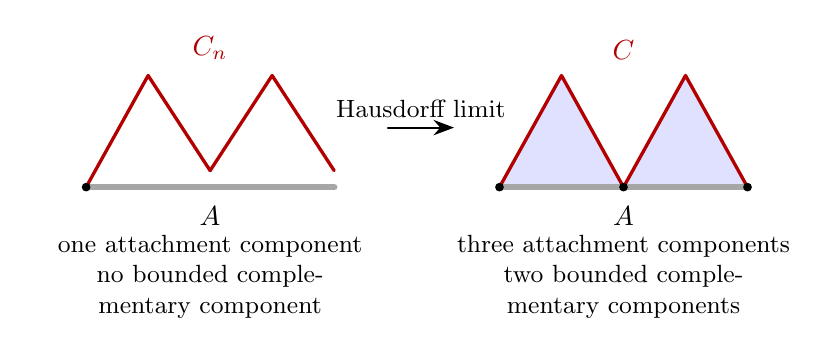
\begin{tikzpicture}[scale=1.05, line cap=round, line join=round]
  \begin{scope}[xshift=-3.8cm]
    \draw[line width=2.4pt,gray!70] (0,0)--(3,0);
    \draw[very thick,red!70!black]
      (0,0)--(.75,1.35)--(1.5,.20)--(2.25,1.35)--(3,.20);
    \fill (0,0) circle (1.5pt);
    \node[below] at (1.5,-.12) {$A$};
    \node[red!70!black,above] at (1.5,1.42) {$C_n$};
    \node[align=center,text width=4.4cm,font=\small] at (1.5,-1.08)
      {one attachment component\\no bounded complementary component};
  \end{scope}
  \begin{scope}[xshift=1.2cm]
    \fill[blue!12] (0,0)--(.75,1.35)--(1.5,0)--cycle;
    \fill[blue!12] (1.5,0)--(2.25,1.35)--(3,0)--cycle;
    \draw[line width=2.4pt,gray!70] (0,0)--(3,0);
    \draw[very thick,red!70!black]
      (0,0)--(.75,1.35)--(1.5,0)--(2.25,1.35)--(3,0);
    \foreach \x in {0,1.5,3} \fill (\x,0) circle (1.5pt);
    \node[below] at (1.5,-.12) {$A$};
    \node[red!70!black,above] at (1.5,1.42) {$C$};
    \node[align=center,text width=4.4cm,font=\small] at (1.5,-1.08)
      {three attachment components\\two bounded complementary components};
  \end{scope}
  \draw[-{Stealth[length=2.6mm]},thick]
    (-.15,.72)--(.65,.72) node[midway,above,font=\small] {Hausdorff limit};
\end{tikzpicture}
\caption{Trace multiplication in Proposition~\ref{prop:trace-birth}, shown
for $m=2$.  Every finite connector $C_n$ meets the atom once, so
$A\cup C_n$ is full.  In the limit, two near-contacts close and the trace
$A\cap C$ has three components.  Formula~\eqref{eq:G-full-budget} detects
the two shaded bounded complementary components exactly.}
\label{fig:trace-birth}
\end{figure}

\subsection{A safe limiting regime}
\label{subsec:G-nested-limit}

The preceding defect is specific to uncontrolled Hausdorff convergence.
There is a useful inverse-limit regime in which neither connector holes nor
trace components can be born.

\begin{theorem}[Nested-limit stability]
\label{thm:nested-limit-stability}
Let $s\ge1$, let $A_1,\dots,A_s\subset\C$ be pairwise disjoint full
continua, and let
\[
 C_1\supset C_2\supset\cdots
\]
be a decreasing sequence of nonempty full continua.  Suppose that
$C_n\cap A_i$ is nonempty and connected for every $n$ and $i$.  Then
\[
 C_\infty:=\bigcap_{n\ge1}C_n
\]
is a full continuum, every trace $C_\infty\cap A_i$ is nonempty and
connected, and
\[
 H_\infty:=C_\infty\cup\bigcup_{i=1}^{s}A_i
\]
is a full continuum.

If, in addition, the data lie in the setup of
Corollary~\ref{cor:continuum-connector}, every $C_n\Subset U$ avoids the
fixed obstacle set, and every $C_n$ satisfies that corollary's
relative-collar clearance conditions, then $H_\infty$
inherits obstacle avoidance and every protected prime-end chain survives
with the same injectivity and cyclic-order conclusions.
\end{theorem}

\begin{proof}
The nested-intersection theorem for continua makes $C_\infty$ nonempty,
compact, and connected.  Moreover
\[
 \Chat\setminus C_\infty
 =
 \bigcup_{n\ge1}(\Chat\setminus C_n).
\]
The sets on the right are connected and increasing, and all contain
$\infty$; their union is connected.  Hence $C_\infty$ is full.

For fixed $i$, the continua $C_n\cap A_i$ are nonempty, compact, connected,
and decreasing.  Their intersection is therefore nonempty and connected,
and distributivity of intersection gives
\[
 \bigcap_n(C_n\cap A_i)=C_\infty\cap A_i.
\]
Corollary~\ref{cor:full-connector-traces} now makes $H_\infty$ full.
Avoidance and relative-collar clearance pass to the subset $C_\infty$;
the final assertion follows from
Corollary~\ref{cor:continuum-connector}.
\end{proof}

The theorem suggests a concrete route for an infinite construction:
produce a \emph{decreasing} system of full connector envelopes with
connected, nonempty traces, rather than take an arbitrary subsequential
Hausdorff limit of finite trees.  It is a sufficient architecture, not a
claim that the dynamical program already supplies such envelopes.

\begin{warning}[The compactness gate]
\label{warn:compactness-gate}
Fullness and singleton attachment traces are not closed under Hausdorff
limits.  Proposition~\ref{prop:trace-birth} isolates the trace-birth
failure, while
\[
C_n=\{e^{it}:1/n\le t\le2\pi\}
\]
are closed arcs converging in Hausdorff distance to the separating Jordan
curve $S^1$, isolating the independent cycle-birth failure in the connector
itself.  Therefore a
finite protected-carrier theorem cannot be passed to an infinite or virtual
horizon by compactness alone.  At minimum, one must prove that the limiting
connector remains nonseparating and that each limiting attachment trace
remains nonempty and connected.  Under exactly those two conclusions,
Corollary~\ref{cor:full-connector-traces} restores fullness of the limiting
carrier.
\end{warning}

The warning is deliberately a no-go statement rather than a promoted
dynamical claim.  It sharpens the finite/infinite boundary of this paper:
the finite certificate solves routing, but a future limiting construction
must control both connector cohomology and trace multiplication.  Neither
control follows from Hausdorff precompactness.  Theorem
\ref{thm:nested-limit-stability} supplies one sufficient replacement:
decreasing full envelopes with nonempty connected traces.
% ---- end G:separation_budget ----

% ---- begin D:criterion ----
% Cluster D: the repaired slit lemma and the exact free-component criterion
% Body-only LaTeX; uses only preamble macros and fixed cross-cluster labels.

\section{The exact free-component criterion}\label{sec:criterion}

Theorem~\ref{thm:realization} converts a protected ribbon-routing certificate into an
actual carrier, but it leaves open the question of when such a certificate exists: the
embedded finite tree of Definition~\ref{def:certificate} looks like an arbitrary choice,
and one might fear that its existence depends on delicate features of the atoms or of the
forbidden data. The present section removes the arbitrary tree choice. We prove that the
existence of a protected ribbon-routing certificate is governed by a single, exact,
purely planar condition: one component of a frozen free domain must reach every required
atom by a singleton port. The section carries the one intentional mathematical divergence
of this paper from the source manuscript \cite{MWman}: the slit lemma below is stated and
proved in a repaired form, and the proof of the criterion is rewritten to match. The
divergence is recorded precisely in Remark~\ref{rem:repair}.

\subsection{The frozen free domain}\label{subsec:D-frozen}

Freeze the complete finite future inventory before choosing a connector.
Concretely, fix $s\ge1$, let $U$ be the Jordan localization, let
$A_1,\dots,A_s\Subset U$ be the pairwise disjoint atoms, and let
$Z\Subset U\setminus\bigcup_iA_i$ be the same compact set of separated
obstacles, critical-value exclusions, and localization-forbidden data used
in Definition~\ref{def:certificate}.  For each atom define its compact
\emph{atom--tail block}
\[
\mathcal B_i:=
A_i\cup\bigcup_a(\overline{D_{i,a,1}}\setminus A_i)
=A_i\cup\bigcup_a\overline{D_{i,a,1}},
\]
and put
\[
Q:=\bigcup_{i=1}^{s}\mathcal B_i\cup Z.
\]
Thus every relative tail is processed together with its atom, even when
different prime-end impressions overlap inside $A_i$.  Each
$\overline{D_{i,a,1}}$ is connected and meets $A_i$ in its nonempty
impression, so $\mathcal B_i$ is a compact connected set (and equals $A_i$ when
there are no protected labels).  The truncation normalization and compact
containment of $Z$ make the finite union $Q\Subset U$ compact.  Put
\begin{equation}\label{eq:D-free-domain}
\Omfree \;=\; U\setminus Q
\end{equation}
(equation~(9.4) of the manuscript \cite{MWman}). The set $\Omfree$ is open, and its
connected components are plane domains, the \emph{free components} of the frozen data.

A component $\Omega_0$ of $\Omfree$ \emph{has simultaneous singleton ports} to the
required atoms if there are pairwise disjoint Jordan arcs
$\alpha_1,\dots,\alpha_s\colon[0,1]\to U$ such that, for every $i$, the arc $\alpha_i$
meets $A_i$ exactly in the single point $x_i=\alpha_i(0)$ and satisfies
$\alpha_i\bigl((0,1]\bigr)\subset\Omega_0$. The landing point $x_i$ is called a
\emph{free point} of $A_i$ because it is reached from the free domain; no further
property of $x_i$ is assumed at this stage. (Compare the unprotected exposure loci of
Lemma~\ref{lem:port-localization}, where an additional protected-impression exclusion is
imposed; the interaction between the two notions is illustrated in
Example~\ref{ex:no-common-component} below.)

The adjective \emph{frozen} is load-bearing, and we emphasize it once. The set $Q$ lists
the complete finite future inventory: every atom that will ever have to be joined, the
relative terminal collar tail of every protected chain that any future step of a proof will
read, every obstacle that must remain separated, the full critical-value exclusion, and
the localization-forbidden set. This list is fixed \emph{before} any connector is chosen.
Nothing may be added to $Q$ afterwards, and nothing may be removed from it; all later
monotone operations act on proposed connectors, never on the inventory. This discipline
is exactly what gives the criterion of Theorem~\ref{thm:free-component} its
if-and-only-if form, and what makes its failure clause persistent: a separation already
visible in the frozen data can never be talked away by enlarging a connector. The
horizon-first closure results of the manuscript \cite{MWman} address how such an
inventory stabilizes; here the inventory is simply given, finite, and immutable.

\subsection{The repaired slit lemma}\label{subsec:D-slits}

The sufficiency direction of the criterion rests on the fact that finitely many pairwise
disjoint one-ended slits do not disconnect a plane domain. This is Lemma~10.7 of the
manuscript. Its printed statement contains a formal inconsistency (a map into an open
domain cannot take a boundary value) together with an endpoint mismatch with its
intended application; both defects are repaired in the statement below, and
Remark~\ref{rem:repair} records the divergence. The mathematical core of the
manuscript's argument --- the transverse-rectangle detour around the free endpoint ---
is retained in full.

\begin{lemma}[One-ended slits do not disconnect a plane domain; manuscript Lemma 10.7,
repaired]\label{lem:slits}
Let $\Omega\subset\C$ be a domain and let
$\delta_1,\dots,\delta_s\colon[0,1]\to\overline{\Omega}$ be Jordan arcs with pairwise
disjoint images such that $\delta_i(0)\in\partial\Omega$ and
$\delta_i\bigl((0,1]\bigr)\subset\Omega$ for every $i$. Then
\[
\Omega\setminus\bigcup_{i=1}^{s}\delta_i\bigl((0,1)\bigr)
\]
is path connected; in particular every free endpoint $\delta_i(1)$ lies in this set and
can be joined inside it to every other point of it.
\end{lemma}

\begin{proof}
Call $\delta_i$ the \emph{$i$-th slit}, write
$\sigma_i:=\delta_i\bigl((0,1]\bigr)$ for its \emph{half-open} part and
$\sigma_i^{\circ}:=\delta_i\bigl((0,1)\bigr)$ for its \emph{open} part, and call
$\delta_i(1)$ its \emph{tip}. The set to be proved path connected is
$\Omega\setminus\bigcup_i\sigma_i^{\circ}$, which contains all $s$ tips. If $s=0$ there
is nothing to prove, so assume $s\ge1$; then $\partial\Omega\neq\varnothing$.

\emph{Step 0: two preliminary observations.}
First, each half-open part $\sigma_i$ is relatively closed in $\Omega$. Indeed, the
closure of $\sigma_i$ in $\C$ is the compact arc $\delta_i([0,1])$, so the only point of
$\overline{\sigma_i}\setminus\sigma_i$ is $\delta_i(0)\in\partial\Omega$, which does not
lie in $\Omega$. Consequently $\Omega\setminus\sigma_i$ is open. By contrast, the open
part $\sigma_i^{\circ}$ is \emph{not} relatively closed in $\Omega$: its closure inside
$\Omega$ also contains the tip $\delta_i(1)\in\Omega$. This distinction is precisely the
point at which the manuscript's induction required repair; the proof below removes the
half-open parts first and reattaches the tips afterwards.

Second, every Jordan arc in the plane is tame: it can be extended to a Jordan curve,
and the Schoenflies theorem then supplies a homeomorphism of $\C$ carrying the curve to
a round circle and the arc to a circular subarc, hence, after one more homeomorphism,
onto the straight segment $[0,1]\times\{0\}$; see, e.g.,
\cite{New51,Why42}. Since path connectivity is a topological invariant and a
homeomorphism of $\C$ carries domains to domains and boundaries to boundaries, we may
straighten any \emph{single} slit whenever convenient. (Straightening one slit will in
general bend the others; each step below straightens only the slit it is processing.)

\emph{Step 1: removing a single half-open slit leaves a domain.}
Let $\Omega$ be a domain and let $\delta$ be a single arc as in the statement, with
half-open part $\sigma=\delta\bigl((0,1]\bigr)$. We claim that
$\Omega':=\Omega\setminus\sigma$ is again a domain. Openness was proved in Step~0, so
only path connectivity is at issue. By tameness we may assume, after a homeomorphism of
$\C$, that
\[
\delta(t)=(t,0)\quad(0\le t\le1),
\]
so that $\Omega$ is a domain containing $S:=(0,1]\times\{0\}$, with
$(0,0)\in\partial\Omega$, and we must join two arbitrary points
$x,y\in\Omega\setminus S$ by a path in $\Omega\setminus S$.

\emph{(a) A polygonal start missing an initial tail.}
Since a plane domain is polygonally connected \cite{New51}, choose a polygonal path
$P\subset\Omega$ from $x$ to $y$. The path $P$ is compact and does not contain the
boundary point $(0,0)$, so
\[
r:=\dist\bigl((0,0),P\bigr)>0 .
\]
Fix $\varepsilon:=\tfrac12\min(r,1)$. Every point of the initial tail
$[0,\varepsilon]\times\{0\}$ lies within distance $\varepsilon<r$ of the origin, so $P$
misses $[0,\varepsilon]\times\{0\}$. This is the only part of the closed slit that a
compact subset of $\Omega$ cannot in general avoid by compactness alone: the closed slit
image leaves every compact subset of $\Omega$ only along points accumulating at
$\delta(0)=(0,0)\in\partial\Omega$, and near that end the continuity of $\delta$ at $0$
confines the slit to a small disk around the origin. The remaining part
$\delta([\varepsilon,1])=[\varepsilon,1]\times\{0\}$ is a compact subset of $\Omega$ and
will be handled by explicit detours.

\emph{(b) A thin rectangle around the compact subarc.}
The segment $[\varepsilon,1]\times\{0\}$ lies in $\Omega$, and $(1,0)\in\Omega$ is an
interior point of $\Omega$; hence there is $\eta\in(0,\tfrac12)$ with
$[1,1+\eta]\times\{0\}\subset\Omega$. The segment
$L:=[\varepsilon/2,\,1+\eta]\times\{0\}$ is then a compact subset of $\Omega$, so
$\dist(L,\C\setminus\Omega)>0$, and we may choose
$h\in\bigl(0,\min(\varepsilon/2,\dist(L,\C\setminus\Omega)/2)\bigr)$ and set
\[
R:=[\varepsilon/2,\,1+\eta]\times[-h,h]\subset\Omega .
\]
The rectangle $R$ meets the closed slit $[0,1]\times\{0\}$ exactly in the core
$c:=[\varepsilon/2,\,1]\times\{0\}$: the slit enters $R$ through the midpoint of its
left short side and terminates at the tip $(1,0)$, an interior point of $R$. In
particular $R\cap S=[\varepsilon/2,1]\times\{0\}=c$.

We record the key connectivity property of the slit rectangle: \emph{$R\setminus c$ is
path connected.} Indeed, let $V:=\{1+\eta/2\}\times[-h,h]$, a vertical segment in $R$
missing $c$. A point of $R\setminus c$ with ordinate $y\neq0$ travels horizontally to
the point of $V$ with the same ordinate; the horizontal path misses the axis
$\mathbb{R}\times\{0\}$ entirely, hence misses $c$. A point of $R\setminus c$ with
ordinate $0$ has abscissa in $(1,1+\eta]$ and travels along the axis to $(1+\eta/2,0)$;
this path keeps abscissa $>1$, hence misses $c$. Since $V$ is connected, the claim
follows. Geometrically: the two long sides of $R$ are joined to each other inside
$R\setminus c$ \emph{around the tip}, by crossing the axis at abscissae beyond $1$.

\emph{(c) Transverse perturbation and detour repair.}
Perturb the interior vertices of $P$, keeping the endpoints $x,y$ fixed, so that no
interior vertex lies on the axis $\mathbb{R}\times\{0\}$ and no edge of $P$ is collinear
with the axis; if an endpoint happens to lie on the axis (necessarily off $S$), perturb
its adjacent vertex so that the incident edge is not horizontal. Since $P$ is compact
with $\dist(P,\C\setminus\Omega)>0$ and $\dist\bigl(P,[0,\varepsilon]\times\{0\}\bigr)
\ge r-\varepsilon>0$, a sufficiently small such perturbation keeps $P$ inside $\Omega$
and away from the initial tail. After the perturbation, every edge of $P$ meets the axis
in at most one point, and every meeting point interior to an edge is a transverse
crossing. Hence $P$ meets $S$ in finitely many points, all of the form $P(t_j)$ with
parameters $0<t_1<\dots<t_m<1$ interior to edges, and all lying in
$( \varepsilon,1]\times\{0\}\subset\Int R$. (If $m=0$, the path $P$ already joins $x$ to
$y$ in $\Omega\setminus S$ and Step~1 is complete.)

By transversality, for each $j$ there is $\rho_j>0$ such that the parameter interval
$[t_j-\rho_j,\,t_j+\rho_j]$ has image in $\Int R$, meets the axis only at $t_j$, and the
two punctured halves of the image lie strictly on opposite sides of the axis; shrink the
$\rho_j$ so that these intervals are pairwise disjoint and avoid $0$ and $1$. Put
$p_j^{-}:=P(t_j-\rho_j)$ and $p_j^{+}:=P(t_j+\rho_j)$; both lie in $R\setminus c$.
Now modify $P$ as follows: on each interval $[t_j-\rho_j,\,t_j+\rho_j]$, replace the
sub-path of $P$ by a path from $p_j^{-}$ to $p_j^{+}$ inside $R\setminus c$, which
exists by (b); keep $P$ unchanged elsewhere. Each detour lies in $R\subset\Omega$ and
misses $S$, because $S\cap R=c$ and the detour misses $c$, while $S\setminus R$ is
disjoint from $R$. The unchanged pieces of $P$ carry parameters outside the intervals
$(t_j-\rho_j,\,t_j+\rho_j)$ and therefore avoid $S$, since the crossings $t_j$ were the
only parameters at which $P$ met $S$. The concatenation is a path from $x$ to $y$ in
$\Omega\setminus S$.

Observe that each detour crosses the axis only at abscissae strictly beyond $1$: it
travels \emph{around} the tip, through points arbitrarily close to $\delta(1)$ but never
through any point of the closed slit; the tip itself, which here has been removed
together with the rest of $\sigma$, is not needed as a way-station. This completes
Step~1: $\Omega'=\Omega\setminus\sigma$ is a domain.

\emph{Step 2: removing all half-open slits leaves a domain.}
Set $\Omega_{(0)}:=\Omega$ and, inductively,
$\Omega_{(j)}:=\Omega_{(j-1)}\setminus\sigma_j$ for $1\le j\le s$. We claim that each
$\Omega_{(j)}$ is a domain and that $\delta_j$ is a one-ended slit of $\Omega_{(j-1)}$
in the sense of the statement. Indeed, suppose $\Omega_{(j-1)}$ is a domain. Because the
slit images are pairwise disjoint, $\sigma_j$ is disjoint from
$\sigma_1,\dots,\sigma_{j-1}$, so $\sigma_j\subset\Omega_{(j-1)}$. The point
$\delta_j(0)$ lies outside $\Omega\supset\Omega_{(j-1)}$, and it is the limit of the
points $\delta_j(t)\in\Omega_{(j-1)}$ as $t\downarrow0$; hence
$\delta_j(0)\in\partial\Omega_{(j-1)}$ and
$\delta_j\colon[0,1]\to\overline{\Omega_{(j-1)}}$. Step~1, applied to the domain
$\Omega_{(j-1)}$ and the single slit $\delta_j$, now shows that $\Omega_{(j)}$ is a
domain. After $s$ steps we conclude: the set
\[
\Omega_{(s)}\;=\;\Omega\setminus\bigcup_{i=1}^{s}\sigma_i
\;=\;\Omega\setminus\bigcup_{i=1}^{s}\delta_i\bigl((0,1]\bigr)
\]
is open and path connected.

\emph{Step 3: reattaching the tips.}
The set whose path connectivity is asserted differs from $\Omega_{(s)}$ exactly by the
$s$ tips:
\[
\Omega\setminus\bigcup_{i=1}^{s}\sigma_i^{\circ}
\;=\;\Omega_{(s)}\,\cup\,\{\delta_1(1),\dots,\delta_s(1)\},
\]
and the tips are pairwise distinct points not in $\Omega_{(s)}$. Since $\Omega_{(s)}$ is
path connected, it suffices to join each tip to some point of $\Omega_{(s)}$ by a path
which, apart from the tip itself, lies in $\Omega_{(s)}$.

Fix $i$ and straighten the $i$-th slit: let $\Phi$ be a homeomorphism of $\C$ with
$\Phi\bigl(\delta_i([0,1])\bigr)=[0,1]\times\{0\}$ and $\Phi(\delta_i(t))=(t,0)$. The
union $K:=\bigcup_{k\neq i}\delta_k([0,1])$ of the other closed slit images is compact
and disjoint from $\delta_i([0,1])$, so $\Phi(K)$ is compact and disjoint from
$[0,1]\times\{0\}$. The model tip $(1,0)$ lies in the open set $\Phi(\Omega)$ and
outside the closed set $\Phi(K)$, so
\[
\mu:=\dist\Bigl((1,0),\,\Phi(K)\cup\bigl(\C\setminus\Phi(\Omega)\bigr)\Bigr)>0 .
\]
Choose $a\in\bigl(0,\min(\mu/2,\tfrac12)\bigr)$ and consider the square
$R_i:=[1-a,\,1+a]\times[-a,a]$. Every point of $R_i$ lies within distance $a\sqrt2<\mu$
of the model tip, so $R_i\subset\Phi(\Omega)$ and $R_i\cap\Phi(K)=\varnothing$; moreover
$R_i$ meets the model slit $[0,1]\times\{0\}$ exactly in $[1-a,1]\times\{0\}$. The
\emph{escape segment}
\[
E_i:=[1,\,1+a/2]\times\{0\}
\]
runs from the model tip into $R_i$; every point of $E_i$ other than the tip has abscissa
$>1$, hence lies on none of the straightened slits, and lies in $R_i$, hence off
$\Phi(K)$. Pulling back, $\beta_i:=\Phi^{-1}(E_i)$ is a Jordan arc from $\delta_i(1)$ to
a point $z_i\in\Omega_{(s)}$ with $\beta_i\setminus\{\delta_i(1)\}\subset\Omega_{(s)}$.
Thus the tip $\delta_i(1)$ lies in the same path component as $z_i$, hence in the path
component of $\Omega_{(s)}$.

The same square makes the two-sided accessibility of the tip transparent: inside
$R_i\setminus\bigl([1-a,1]\times\{0\}\bigr)$ the two long sides of $R_i$ are joined
around the tip by the vertical segment at abscissa $1+a/2$, so the tip is accessible
from either side of the slit, and both accesses land in one and the same path component
of the complement. Finally, note that the escape arc $\beta_i$ can be made arbitrarily
small: shrinking $a$ shrinks $E_i$ to the model tip, and continuity of $\Phi^{-1}$ then
confines $\beta_i$ to any prescribed neighborhood of $\delta_i(1)$.

\emph{Step 4: conclusion.}
By Steps 2 and 3 the set
$\Omega\setminus\bigcup_i\sigma_i^{\circ}=\Omega_{(s)}\cup\{\delta_1(1),\dots,
\delta_s(1)\}$ is path connected, and it contains every free endpoint $\delta_i(1)$;
each of these can therefore be joined inside it to every other point of it.
\end{proof}

Two by-products of the proof will be used in the proof of
Theorem~\ref{thm:free-component} and are worth recording explicitly. First, by Step~2,
removing the \emph{half-open} slits $\delta_i((0,1])$ leaves an open, path connected
set --- indeed a plane domain, hence a polygonally connected one. Second, by Step~3,
every tip $\delta_i(1)$ admits arbitrarily small escape arcs: for every neighborhood $N$
of $\delta_i(1)$ there is a Jordan arc $\beta\subset N$ from $\delta_i(1)$ into the slit
complement with $\beta\setminus\{\delta_i(1)\}\subset
\Omega\setminus\bigcup_k\delta_k\bigl((0,1]\bigr)$.

\begin{remark}[The repair]\label{rem:repair}
We record the divergence from the printed manuscript statement \cite{MWman}. Manuscript
Lemma~10.7 states the hypothesis in the form
$\delta_i\colon[0,1]\to\Omega$ with $\delta_i(0)\in\partial\Omega$, which is formally
inconsistent: a map into the open domain $\Omega$ cannot take a boundary value. It then
removes the half-open slits $\delta_i\bigl((0,1]\bigr)$, \emph{including} the free
endpoints $\delta_i(1)$, while the manuscript's proof of Theorem~10.8 (reproduced as
Theorem~\ref{thm:free-component} below) joins precisely those outer endpoints by paths
inside the complement --- an endpoint mismatch: the points to be joined have just been
deleted. The statement of Lemma~\ref{lem:slits} repairs both defects at once: the
codomain is $\overline{\Omega}$, so the initial boundary value is legitimate, and only
the open arcs $\delta_i\bigl((0,1)\bigr)$ are removed, so the free endpoints remain
available for routing.

A third, smaller point is repaired inside the proof. The manuscript's induction asserts
that the removed slit is relatively closed in $\Omega$, so that the complement is again
a domain and the one-slit argument iterates. For the half-open slit
$\delta_i\bigl((0,1]\bigr)$ this is true (Step~0), but for the open slit
$\delta_i\bigl((0,1)\bigr)$ it is false: the closure inside $\Omega$ adds the tip, so
the complement of the open slit is not open at the tip and the inductive step cannot be
applied verbatim to the repaired statement. The proof above therefore removes the
half-open slits one at a time (Steps~1 and~2), where relative closedness does hold, and
reattaches the $s$ retained tips afterwards by the tip-accessibility argument (Step~3).

The repair changes no application. Every invocation of the lemma in the source
manuscript --- and every invocation in this paper --- uses exactly the repaired form:
the slits to be removed are open port interiors, and the retained outer endpoints are
then joined inside the complement. The transverse-rectangle detour, which is the
mathematical core of the manuscript's one-slit argument, is unchanged.
\end{remark}

\subsection{The criterion}\label{subsec:D-criterion}

\begin{theorem}[Protected Free-Component Criterion; manuscript Theorem 10.8]
\label{thm:free-component}
A protected ribbon-routing certificate exists if and only if one component of $\Omfree$
has simultaneous singleton ports to every required atom.  Consequently, if
$Q$ is fixed and no component has such ports, no enlargement of a proposed
connector that continues to respect the same frozen inventory can become a
protected ribbon-routing certificate.
\end{theorem}

\begin{proof}
\emph{Necessity.}
Let a protected ribbon-routing certificate be given, with free-port arcs
$\alpha_1,\dots,\alpha_s$, landing points $x_i=\alpha_i(0)\in A_i$, and embedded finite
tree $G$ joining the outer port endpoints (Definition~\ref{def:certificate}). Delete the
atoms from the connector and consider
\[
X\;:=\;G\,\cup\,\bigcup_{i=1}^{s}\alpha_i\bigl((0,1]\bigr).
\]
The tree $G$ is connected, and each half-open port arc $\alpha_i\bigl((0,1]\bigr)$ is a
connected set containing the outer endpoint $\alpha_i(1)\in G$; hence $X$ is connected.
Moreover $X\subset\Omfree$: by Definition~\ref{def:certificate}, the sets
$\alpha_i\bigl((0,1]\bigr)$ and $G$ lie in $U$ and avoid every atom, the obstacle and
critical-value set, and every relative terminal protected collar tail.  The
localization-forbidden data are part of $Z$ by the convention of
Section~\ref{sec:certificates}.  The avoided sets are therefore exactly the
constituents of $Q$. A
connected subset of the open set $\Omfree$ lies in a single component $\Omega_0$. The
certificate's own port arcs are then simultaneous singleton ports of $\Omega_0$: they
are pairwise disjoint Jordan arcs, $\alpha_i$ meets $A_i$ exactly in $\{x_i\}$, and
$\alpha_i\bigl((0,1]\bigr)\subset X\subset\Omega_0$.

\emph{Sufficiency.}
Conversely, let $\Omega_0$ be a component of $\Omfree$ with simultaneous singleton ports
$\alpha_1,\dots,\alpha_s$. Fix $\tau\in(0,1]$ and shorten each port away from the atoms,
replacing $\alpha_i$ by its initial subarc $\alpha_i|_{[0,\tau]}$, reparametrized over
$[0,1]$ and still denoted $\alpha_i$; the shortened arcs remain pairwise disjoint
simultaneous singleton ports, and the shortening emphasizes that only the germ of each
port at its atom matters. Write $y_i:=\alpha_i(1)$ for the retained outer endpoints.

The shortened ports are one-ended slits of the domain $\Omega_0$ in the sense of
Lemma~\ref{lem:slits}. Indeed, their images are pairwise disjoint; the interiors satisfy
$\alpha_i\bigl((0,1]\bigr)\subset\Omega_0$; and the landing point
$x_i=\alpha_i(0)$ lies in $A_i\subset Q$, hence outside $\Omega_0$, while being the
limit of the points $\alpha_i(t)\in\Omega_0$, so that $x_i\in\partial\Omega_0$ and
$\alpha_i\colon[0,1]\to\overline{\Omega_0}$. The retained port interiors are therefore
finitely many pairwise disjoint one-ended slits of $\Omega_0$, and
Lemma~\ref{lem:slits} applies to remove their \emph{open} parts: the set
\[
W\;:=\;\Omega_0\setminus\bigcup_{i=1}^{s}\alpha_i\bigl((0,1)\bigr)
\]
is path connected, and it contains the outer endpoints $y_1,\dots,y_s$ --- which is
exactly what the repaired statement guarantees.

We now upgrade the joining paths supplied by path connectivity of $W$ to an embedded
polygonal tree, using the two by-products recorded after the proof of
Lemma~\ref{lem:slits}. First, by Step~2 of that proof,
\[
\Omega'\;:=\;\Omega_0\setminus\bigcup_{i=1}^{s}\alpha_i\bigl((0,1]\bigr)
\]
is a plane domain. Second, by Step~3, each tip $y_i$ admits arbitrarily small escape
arcs into $\Omega'$. If $s=1$, choose such an escape arc $\beta_1$ from
$y_1$ to a point $z_1\in\Omega'$, replace the port by
$\alpha_1*\beta_1$, and take the degenerate one-vertex tree
$G=\{z_1\}$.  The incidence and avoidance clauses are then immediate, so
this is a certificate.  Assume henceforth that $s\ge2$. Let
$\rho:=\tfrac13\min_{i\neq j}|y_i-y_j|>0$, and choose for each
$i$ an escape arc $\beta_i\subset B(y_i,\rho)$ with $\beta_i(0)=y_i$ and
$\beta_i\bigl((0,1]\bigr)\subset\Omega'$; the balls $B(y_i,\rho)$ are pairwise
disjoint, so the arcs $\beta_i$ are pairwise disjoint. Put $z_i:=\beta_i(1)\in\Omega'$.

Since the domain $\Omega'$ is polygonally connected, choose polygonal paths
$P_2,\dots,P_s\subset\Omega'$ joining $z_1$ to $z_2,\dots,z_s$. Perturb them, keeping
their endpoints fixed, into general position inside $\Omega'$: after an arbitrarily
small perturbation, any two edges taken from distinct paths, or nonadjacent edges of one
path, meet in at most one point and transversely, and no vertex of one path lies on
another path except at shared endpoints. The union $\Gamma:=P_2\cup\dots\cup P_s$ is
then a connected finite plane graph in $\Omega'$ containing $z_1,\dots,z_s$: its
vertices are the path endpoints together with the finitely many transverse crossings, at
which we subdivide. Let $G_0\subset\Gamma$ be an inclusion-minimal connected subgraph
containing $\{z_1,\dots,z_s\}$. Then $G_0$ is a finite tree: were it to contain a
cycle, deleting one edge of the cycle would leave a connected subgraph still containing
every $z_i$, contradicting minimality. Being a subgraph of an embedded graph, $G_0$ is
embedded, and $G_0\subset\Omega'$.

The escape arcs may meet $G_0$ before their endpoints, so we trim them by a first-hit
argument. For each $i$ the set $\{t\in[0,1]:\beta_i(t)\in G_0\}$ is closed, and it is
nonempty because $\beta_i(1)=z_i\in G_0$; let $t_i^{*}$ be its minimum. Since
$\beta_i(0)=y_i\notin\Omega'\supset G_0$ we have $t_i^{*}>0$. Set
$\beta_i':=\beta_i|_{[0,t_i^{*}]}$ and $z_i':=\beta_i(t_i^{*})\in G_0$, so that
$\beta_i'\cap G_0=\{z_i'\}$.

Assemble the certificate. Define the rerouted port arcs
$\tilde\alpha_i:=\alpha_i*\beta_i'$ for $1\le i\le s$, the concatenation of $\alpha_i$
and $\beta_i'$, reparametrized over $[0,1]$. Each $\tilde\alpha_i$ is a Jordan arc: both
pieces are Jordan arcs meeting exactly at $y_i=\alpha_i(1)=\beta_i'(0)$, because
$\beta_i'\setminus\{y_i\}\subset\Omega'$ while the image
$\alpha_k([0,1])$ of every port lies in
$Q\cup\bigcup_j\alpha_j\bigl((0,1]\bigr)$, a set disjoint from $\Omega'$. The same
disjointness, together with the pairwise disjoint balls containing the $\beta_i$, shows
that $\tilde\alpha_1,\dots,\tilde\alpha_s$ are pairwise disjoint. Each $\tilde\alpha_i$
meets $A_i$ exactly in $\{x_i\}$, and its interior satisfies
$\tilde\alpha_i\bigl((0,1]\bigr)\subset\Omega_0\subset\Omfree$: it avoids every atom,
every relative terminal protected collar tail, the obstacle and critical-value set, and the
localization-forbidden set --- exactly the avoidance clauses that
Definition~\ref{def:certificate} imposes on free-port arcs. Next, subdivide $G_0$ so
that each $z_i'$ is a vertex, and call the resulting embedded finite tree $G$. Then
$G\subset\Omega'$ avoids the same forbidden sets, joins the outer port endpoints
$z_1',\dots,z_s'$, and meets each port arc $\tilde\alpha_i$ exactly in its outer
endpoint $z_i'$, by the first-hit property and $G\subset\Omega'$. Consequently
$G\cup\bigcup_i\tilde\alpha_i$ is again a finite tree: it is connected, and attaching
finitely many pairwise disjoint arcs to a tree, each along a single endpoint, adds one
vertex and one edge at a time and so preserves the tree characterization
$(\text{vertices})-(\text{edges})=1$ for connected finite graphs. The planar cyclic
order of half-edges at every vertex is the one induced by the embedding, and it is
retained as the certificate's ribbon datum. Finally, the protected prime-end crosscut
chains, with their pairwise disjoint relative terminal collar tails, belong to the frozen
inventory and are avoided as recorded above. All clauses of
Definition~\ref{def:certificate} are satisfied: the rerouted ports $\tilde\alpha_i$
together with the spanning tree $G$ constitute a protected ribbon-routing certificate.
Theorem~\ref{thm:realization} now realizes it by a compact connected full carrier with
singleton attachment traces, protected crosscut survival, and preserved cyclic order.

\emph{Persistence.}
For the final assertion, suppose that no component of $U\setminus Q$ has
simultaneous singleton ports to every required atom.  Let a proposed
connector be enlarged in any way that retains the same $Q$ and continues
to satisfy the certificate's avoidance requirements.  If the enlarged
data formed a certificate, the necessity argument would place its connected
routing part in one component of $U\setminus Q$ and would make its own port
arcs simultaneous singleton ports from that component, contrary to the
hypothesis.  Thus no such enlargement can become a certificate.  Changing
this conclusion requires changing the frozen inventory itself, which is
outside the asserted operation.
\end{proof}

The construction is natural under univalent changes of the Jordan localization. An
orientation-preserving conformal homeomorphism of Jordan disks extends over the Jordan
boundaries, and it carries the frozen set $Q$, the free domain \eqref{eq:D-free-domain}
and its components, the port arcs, the escape arcs, and the spanning tree to their
transported counterparts; the transported data form a certificate for the transported
inventory, and the realized carriers correspond as in
Proposition~\ref{prop:naturality}. At the same time the criterion is qualitative: the
number of ports and of ribbon sides is not bounded uniformly, and no width, modulus, or
incidence estimate enters at any point. Nothing in this section constructs the frozen
inventory of a dynamical situation; the corresponding virtual free-component questions
are stated in the source manuscript only as open problems \cite{MWman}, and no part of
this paper bears on them.

\subsection{A separator between individually accessible atoms}\label{subsec:D-example}

The criterion of Theorem~\ref{thm:free-component} is strictly stronger than every
atom-by-atom access condition. The following example, promised in the introduction,
exhibits two atoms each of which passes every individual-access audit, while no common
free component exists; it is the minimal model of the failure mode that the persistence
clause certifies. See Figure~\ref{fig:separation}.

\begin{example}[Individual accesses without a common free component]
\label{ex:no-common-component}
Let $U:=\{z\in\C:|z|<2\}$ and take the two atoms
\[
A_1:=\bigl[-\tfrac14,\tfrac14\bigr],
\qquad
A_2:=\bigl[\tfrac54,\tfrac74\bigr],
\]
closed segments of the real axis, each a full continuum compactly contained in $U$.
Freeze exactly one further inventory item, the round circle
\[
C:=\{z:|z|=1\},
\]
recorded as a separated obstacle; all that matters below is that $C\subset Q$, so any
recording of $C$ in the frozen inventory would do. There
are no critical values and no further forbidden data, so the frozen set is
$Q=A_1\cup A_2\cup C$ and
\[
\Omfree=U\setminus(A_1\cup A_2\cup C).
\]

\emph{The free domain has exactly two components, one per atom.} Write
\[
\Omega_{\mathrm{in}}:=\{|z|<1\}\setminus A_1,
\qquad
\Omega_{\mathrm{ann}}:=\{1<|z|<2\}\setminus A_2,
\]
so that $\Omfree=\Omega_{\mathrm{in}}\sqcup\Omega_{\mathrm{ann}}$, a disjoint union of
open sets separated by the circle $C$. Each is connected, by an explicit radial--angular
path argument. In $\Omega_{\mathrm{in}}$, every point can be joined to the circle
$\{|z|=\tfrac12\}$, which misses $A_1$: a point with $\arg z\notin\{0,\pi\}$ travels
radially to modulus $\tfrac12$, and the radial path keeps its argument, hence stays off
the real axis and misses the real segment $A_1$; a real point of
$\Omega_{\mathrm{in}}$ has modulus in $(\tfrac14,1)$ and travels radially to modulus
$\tfrac12$ through real points of modulus $>\tfrac14$, which also miss $A_1$. In
$\Omega_{\mathrm{ann}}$, every point can be joined to the circle $\{|z|=\tfrac98\}$,
which misses $A_2$: a point with $\arg z\neq0$ travels radially, inward or
outward as needed, keeping its
argument; a positive real point of $\Omega_{\mathrm{ann}}$ has modulus in
$(1,\tfrac54)\cup(\tfrac74,2)$, and in the first case it travels radially to
modulus $\tfrac98$ through positive real points of modulus $<\tfrac54$, while in the
second case it first travels along its own circle $\{|z|=\mathrm{const}\}$ (which
misses $A_2$, as $\tfrac74<|z|<2$) to argument $\pi$ and then proceeds radially inward
as before. Both sets are
therefore domains, and they are exactly the two components of $\Omfree$.

\emph{Every individual-access audit passes.} Exhibit the singleton ports
\[
\alpha_1(t):=\tfrac14+\tfrac t2,
\qquad
\alpha_2(t):=\tfrac74+\tfrac t8
\qquad(0\le t\le1):
\]
the arc $\alpha_1$ runs from $x_1=\tfrac14\in A_1$ to $\tfrac34$ and meets $A_1$ only at
$x_1$, with $\alpha_1\bigl((0,1]\bigr)=(\tfrac14,\tfrac34]\subset\Omega_{\mathrm{in}}$;
the arc $\alpha_2$ runs from $x_2=\tfrac74\in A_2$ to $\tfrac{15}8$ and meets $A_2$ only
at $x_2$, with
$\alpha_2\bigl((0,1]\bigr)=(\tfrac74,\tfrac{15}8]\subset\Omega_{\mathrm{ann}}$. Thus
each atom has a singleton port into \emph{its own} free component. In the language of
the port audit, with empty protected marking and with the atoms as their own completed
packets, both unprotected exposure loci are nonempty, so the hypotheses of
Lemma~\ref{lem:port-localization} hold and its conclusion is correct: the two arcs can
be (and are) chosen pairwise disjoint with interiors in the common complement of the
packets. Atom by atom, nothing is wrong.

\emph{No common free component exists.} Every port of $A_1$ runs in
$\Omega_{\mathrm{in}}$: if $\alpha$ is an arc with
$\alpha\cap A_1=\{\alpha(0)\}$ and $\alpha((0,1])$ contained in one component of
$\Omfree$, then $\alpha(t)\to\alpha(0)\in A_1\subset\{|z|\le\tfrac14\}$ forces
$|\alpha(t)|<1$ for small $t$, so the component is $\Omega_{\mathrm{in}}$. Likewise
every port of $A_2$ runs in $\Omega_{\mathrm{ann}}$, since points of $\Omfree$ near
$A_2$ have modulus in $(1,2)$. As $\Omega_{\mathrm{in}}\neq\Omega_{\mathrm{ann}}$, no
component of $\Omfree$ has simultaneous singleton ports to both atoms, and
Theorem~\ref{thm:free-component} yields: \emph{no protected ribbon-routing certificate
exists} for this frozen inventory.  By the theorem's final assertion, no
connector enlargement that continues to respect this fixed $Q$ can become a
certificate.  The only cure
would be to delete $C$ from the frozen inventory --- a revision of the frozen data,
which the formalism forbids.
\end{example}

The example separates two layers of the theory cleanly. The hypotheses of
Lemma~\ref{lem:port-localization} --- individual exposure of every atom --- are
statements about each atom in isolation, and they hold here; the criterion of
Theorem~\ref{thm:free-component} is a statement about one common component, and it
fails. This is also precisely why Definition~\ref{def:packet} demands that the
completed packets be pairwise disjoint \emph{and cover $Q$}: the separator $C$ must be
assigned to some packet.  Assigning $C$ to a separated-obstacle packet
gives $\Fill(C)=\{|z|\le1\}\supset A_1$, a packet merger with the completed
packet of $A_1$, and this merger is persistent by
Theorem~\ref{thm:audit}.  Assigning $C$ directly to either atom label makes
the corresponding raw seed disconnected, so clause~(1) of the packet
definition fails unless additional declared connecting material is included
in the frozen packet input.  Adding such material changes the input and
requires a fresh audit; it is not a repair of the fixed assignment.
Thus the packet formalism detects the obstruction consistently with the
exact criterion, although only the obstacle-label case invokes the
theorem's monotone-persistence conclusion.

\begin{figure}[t]
\centering
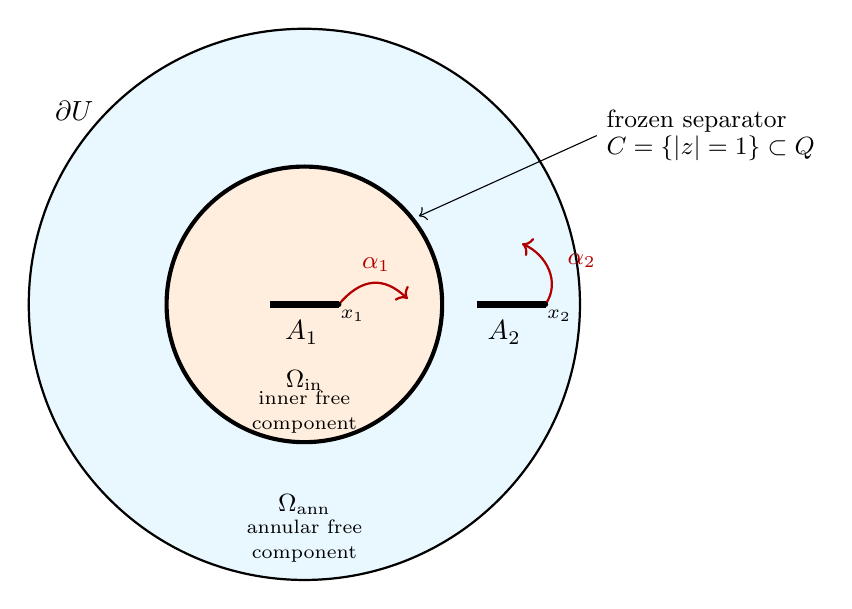
\begin{tikzpicture}[scale=1.75]
% free components, lightly shaded in different tints
\fill[cyan!9,even odd rule] (0,0) circle (2) (0,0) circle (1);
\fill[orange!13] (0,0) circle (1);
% localization boundary
\draw[thick] (0,0) circle (2);
\node at (140:2.18) {$\partial U$};
% the frozen separator, drawn bold
\draw[line width=1.5pt] (0,0) circle (1);
\draw[<-,shorten <=1.5pt] (38:1.02) -- (30:2.45)
  node[right,align=left] {\small frozen separator\\[-2pt]\small $C=\{|z|=1\}\subset Q$};
% atoms
\draw[line width=2.6pt] (-0.25,0) -- (0.25,0);
\node[below] at (-0.02,-0.05) {$A_1$};
\draw[line width=2.6pt] (1.25,0) -- (1.75,0);
\node[below] at (1.45,-0.05) {$A_2$};
% port arcs, one inside each free component
\draw[->,thick,red!70!black] (0.25,0) .. controls (0.42,0.20) and (0.58,0.20) .. (0.75,0.04);
\node[above,red!70!black] at (0.52,0.17) {\small $\alpha_1$};
\fill (0.25,0) circle (0.55pt);
\node[below right,inner sep=1pt] at (0.24,-0.02) {\scriptsize $x_1$};
\draw[->,thick,red!70!black] (1.75,0) .. controls (1.86,0.16) and (1.76,0.36) .. (1.58,0.44);
\node[right,red!70!black] at (1.84,0.32) {\small $\alpha_2$};
\fill (1.75,0) circle (0.55pt);
\node[below right,inner sep=1pt] at (1.74,-0.02) {\scriptsize $x_2$};
% component labels
\node at (0,-0.55) {\small $\Omega_{\mathrm{in}}$};
\node[align=center] at (0,-0.78) {\scriptsize inner free\\[-3pt]\scriptsize component};
\node at (0,-1.45) {\small $\Omega_{\mathrm{ann}}$};
\node[align=center] at (0,-1.72) {\scriptsize annular free\\[-3pt]\scriptsize component};
\end{tikzpicture}
\caption{The separation example of Example~\ref{ex:no-common-component}. The Jordan
localization is the disk $U=\{|z|<2\}$; the frozen inventory consists of the two atoms
$A_1=[-\frac14,\frac14]$ and $A_2=[\frac54,\frac74]$ and the bold circle $C$, a
frozen separator belonging to $Q$. The free domain $\Omfree=U\setminus Q$ has
exactly two components, shaded in different tints: the inner component
$\Omega_{\mathrm{in}}$ and the annular component $\Omega_{\mathrm{ann}}$. Each atom has
a singleton port arc ($\alpha_1$, $\alpha_2$) into its own component, so every
individual-access audit passes; but no single component ports to both atoms, so by
Theorem~\ref{thm:free-component} no protected ribbon-routing certificate exists, and by
the persistence clause no monotone connector enlargement inside $U$ can repair the
failure while $C$ stays in the frozen inventory.}
\label{fig:separation}
\end{figure}
% ---- end D:criterion ----

% ---- begin E:packets ----
% Cluster E, part 1: augmented atoms and the common-domain theorem
% Body-only LaTeX; uses only preamble macros and fixed cross-cluster labels.

\section{Augmented atoms and the common domain}\label{sec:packets}

The free-component criterion of Theorem~\ref{thm:free-component} is exact, and its
persistence clause makes failures permanent; but as a \emph{positive} test it is
expensive. Deciding whether one component of $\Omfree$ reaches every required atom
demands a global analysis of how each of the finitely many collars, obstacles, and
exclusions of the frozen inventory sits relative to all of the others, and
Example~\ref{ex:no-common-component} shows that no atom-by-atom inspection can
substitute for that analysis: individual accessibility of every atom is compatible
with an unrepairable separation. From a \emph{partial} package --- the situation in
which the criterion would actually be invoked, with the inventory delivered piecemeal
by an ambient proof program --- the exact free-domain test is therefore difficult to
verify directly \cite{MWman}.

The present section proves a sufficient criterion that is \emph{source-checkable}:
each of its clauses is verified against named, finite source data rather than against
the component structure of an open set. The idea is to reverse the direction of the
analysis. Instead of asking how the frozen set $Q$ decomposes the localization, we
package $Q$ itself into finitely many pairwise disjoint full continua --- each atom
augmented by the inventory pieces assigned to it, the remainder grouped into
separated-obstacle packets --- while reserving one free port for each original atom.
Once the completed packets are pairwise disjoint, sphere duality forces their common
complement to be \emph{connected}; connectedness, not component bookkeeping, then
delivers the common free component that Theorem~\ref{thm:free-component} demands.

The section has three parts. Definition~\ref{def:packet} fixes the packet structure
and its typed assignment record; Lemma~\ref{lem:packets} is the duality argument; and
Theorem~\ref{thm:common-domain} assembles the sufficient criterion. How the completed
packets are actually computed from raw assigned pieces, and how their defining clauses
are audited with persistent failure certificates, is the subject of
Section~\ref{sec:audit}; Example~\ref{ex:merger} there shows why the audit must be run
on the completions and not on the raw pieces.

\subsection{Filled hulls and augmented packets}\label{subsec:E-packet-def}

Recall from Section~\ref{sec:prelim} the filled hull of a compact plane set $K$:
\begin{equation}\label{eq:E-fill}
\Fill(K)\;=\;K\,\cup\,\bigcup\bigl\{\,B : B\ \text{a bounded component of}\
\C\setminus K\,\bigr\}
\end{equation}
(equation~(9.5) of \cite{MWman}). Since $K$ is compact, $\C\setminus K$ has exactly
one unbounded component $\Omega_\infty(K)$, and \eqref{eq:E-fill} says
\[
\Fill(K)\;=\;\C\setminus\Omega_\infty(K).
\]
Consequently $\Fill(K)$ is closed, and it is bounded because every closed round disk
containing $K$ has its exterior inside $\Omega_\infty(K)$; thus $\Fill(K)$ is compact.
Its complement is the single connected set $\Omega_\infty(K)$, so $\Fill(K)$ is
\emph{full}, and it is the smallest full compact set containing $K$: if $F\supset K$
is full and compact, then $\C\setminus F$ is a connected unbounded subset of
$\C\setminus K$, hence contained in $\Omega_\infty(K)$, which gives
$\Fill(K)\subset F$ after taking complements.  Here neither $K$ nor its
filled hull is asserted to be connected; this least-full-compact statement
does not produce the least full \emph{continuum} ruled out by
Theorem~\ref{thm:no-least}.  Finally, if $K$ is a continuum, then so
is $\Fill(K)$: every bounded component $B$ of $\C\setminus K$ has
$\partial B\subset K$, so its closure $\overline B$ is a connected set meeting $K$,
and $\Fill(K)=K\cup\bigcup\overline B$ is a union of connected sets all meeting the
connected set $K$. The passage from $K$ to $\Fill(K)$ is what the manuscript calls
\emph{fullification}; its algebra --- and in particular the fact that interleaved
adjoin-and-fill operations compute a well-defined completion --- is developed in
Section~\ref{sec:audit}.

Throughout, $s\ge1$, and the \emph{atoms}
$A_1,\dots,A_s\Subset U$ are the pairwise disjoint full
continua of Section~\ref{sec:certificates} that the connector must join, and $Q$ is
the frozen set of Section~\ref{sec:criterion} (equation~(9.4) of \cite{MWman}): the
union of the atoms, the relative terminal protected collar tails, the separated obstacles,
the critical-value exclusion, and the localization-forbidden set, fixed once and for
all before any connector is chosen.  Retain the compact atom--tail blocks
$\mathcal B_i$ of Section~\ref{subsec:D-frozen}, and choose a finite named compact
decomposition $Z=Z_1\cup\cdots\cup Z_N$ of the remaining frozen set
(the one-piece decomposition is allowed; if $Z=\varnothing$, take $N=0$
and no $Z_r$).  The packet input pieces are
the $\mathcal B_i$ and the $Z_r$; a bare relative collar tail, which need not be
compact, is never processed separately.

\begin{definition}[Augmented-atom packet; manuscript Definition 10.9]\label{def:packet}
For the frozen set $Q$, an \emph{augmented-atom packet} consists of full continua
\[
\widehat A_1,\dots,\widehat A_s,\
\widehat O_1,\dots,\widehat O_t\;\Subset\;U
\]
and pairwise disjoint port arcs $\alpha_i\colon[0,1]\to U$ such that:
\begin{enumerate}
\item each atom--tail block $\mathcal B_i$ is assigned to its own atom label, every
named compact constituent $Z_r$ has exactly one assignment to an atom or
separated-obstacle label, and every resulting atom seed $\mathcal B_i\cup E_i$ and
obstacle seed $O_\ell$ is nonempty, compact, and connected;
\item $\widehat A_i=\Fill(\mathcal B_i\cup E_i)$ for every $i$, and
$\widehat O_\ell=\Fill(O_\ell)$ for every $\ell$;
\item the completed packets
$\widehat A_1,\dots,\widehat A_s,\widehat O_1,\dots,\widehat O_t$ are pairwise
disjoint and cover $Q$; and
\item $\alpha_i(0)=x_i\in A_i$, $\alpha_i\cap\widehat A_i=\{x_i\}$, and
\[
\alpha_i\bigl((0,1]\bigr)\;\subset\;
U\setminus\Bigl(\bigcup_{k}\widehat A_k\cup\bigcup_{\ell}\widehat O_\ell\Bigr),
\]
and $x_i$ belongs to no impression of a protected chain.
\end{enumerate}
The \emph{typed assignment} is the resulting function from the finitely
many input pieces $\mathcal B_i,Z_r$ to the atom and separated-obstacle packet
labels, with each $\mathcal B_i$ fixed at label $i$.
\end{definition}

Some commentary on the four clauses. In clause~(1), $E_i$ denotes the
union of the compact $Z_r$ assigned to the $i$-th atom; it may be empty,
and the clause demands that the resulting \emph{atom seed}
$\mathcal B_i\cup E_i$ be compact and connected, so that an assigned piece
disjoint from its block must be accompanied by connecting material assigned
to the same label.  The assignment is load-bearing: it is what makes a later
change of packet label an explicit, auditable re-decision rather than a silent repair, a point
Example~\ref{ex:merger} makes concrete.

In clause~(2), fullness of the completed packets is automatic: the seeds are compact
and connected, so their filled hulls are full continua by the discussion following
\eqref{eq:E-fill}. Clause~(3) is the substantive geometric hypothesis, and it is
stated for the \emph{completed} packets $\widehat A_i,\widehat O_\ell$, not for the
raw seeds: fullification can create intersections that the seeds do not have, and an
audit run at seed level certifies nothing (Example~\ref{ex:merger}). Coverage of $Q$
means that every item of the frozen inventory lies inside some completed packet, so
that outside the packets there is no frozen material at all --- this is the inclusion
that will place the common complement inside $\Omfree$. Clause~(4) is the port
clause. It is deliberately stronger than the port clause of
Definition~\ref{def:certificate}: the arc's positive-parameter part must avoid every
completed hull, whereas the arcs of Definition~\ref{def:certificate} avoid only the
obstacle set, the atoms, and the relative terminal collar tails, and the arc here must meet
even its own augmented atom $\widehat A_i$ only at the landing point $x_i$. The final requirement,
that $x_i$ belong to no impression of a protected chain, keeps the port compatible with
the protected marking; it reappears in Section~\ref{sec:audit} as the requirement
that $x_i$ lie in the unprotected exposure locus, outside the forbidden impression
set $P_i$.

\subsection{Nonseparation of finite disjoint full families}\label{subsec:E-duality}

The engine of the common-domain theorem is a nonseparation statement for finitely
many disjoint full continua on the sphere. Here a compact set $K\subset S^2$ is
called full when $S^2\setminus K$ is connected; for a compact subset of the plane
this agrees with the planar notion, because adjoining the point at infinity to the
unbounded complementary component does not change connectivity, so a plane-full
compact set is sphere-full and conversely. The proof uses the compacta form of
Alexander duality \cite[Chapter~6]{Spa66}:
\begin{equation}\label{eq:E-duality}
\widetilde H_0\bigl(S^2\setminus K;\Z\bigr)\;\cong\;\check H^1(K;\Z)
\end{equation}
for an arbitrary nonempty proper compact subset $K\subset S^2$ (equation~(9.6) of
\cite{MWman}). The \v{C}ech form, rather than the locally contractible special case,
is required here: the atoms and the raw packet seeds are arbitrary continua,
no local connectivity is assumed anywhere in this paper, and for such compacta
singular cohomology need not compute the group on the right of
\eqref{eq:E-duality}.

\begin{remark}\label{rem:E-cech}
The insistence on the \v{C}ech form is not pedantry but a structural feature of the
framework. Clause~(6) of Theorem~\ref{thm:realization} promises that no local
connectivity of any atom is ever required, and the packets of
Definition~\ref{def:packet} inherit whatever boundary pathology their atoms and
assigned pieces possess. \v{C}ech cohomology is the invariant that remains dual to
the complement's component count for every compact subset of the sphere, without any
tameness hypothesis; every duality argument below is stated so that it factors
through \eqref{eq:E-duality} alone.
\end{remark}

\begin{lemma}[Finite disjoint full packets; manuscript Lemma 10.10]\label{lem:packets}
If $K_0,\dots,K_N\subsetneq S^2$ are pairwise disjoint nonempty full
continua, then
\[
S^2\setminus\bigcup_{r=0}^{N}K_r
\]
is connected.
\end{lemma}

\begin{proof}
Write $X:=\bigcup_{r=0}^{N}K_r$.  The set $X$ is a proper subset of
$S^2$, so that \eqref{eq:E-duality} applies to $X$ and to each $K_r$: were $X=S^2$,
the sets $K_0,\dots,K_N$ would be finitely many pairwise disjoint nonempty closed
sets covering $S^2$; each would then be open as well, being the complement of the
union of the others, and connectedness of $S^2$ would force $N=0$ and $K_0=S^2$, in
contradiction with $K_0\subsetneq S^2$.

\emph{Step 1: each packet has vanishing first \v{C}ech cohomology.}
Fix $r$. Fullness of $K_r$ makes $S^2\setminus K_r$ connected, and it is nonempty
because $K_r$ is proper. Being open in $S^2$, the complement is locally path
connected, so connectedness makes it path connected and its reduced zeroth singular
homology vanishes. Hence \eqref{eq:E-duality}, applied to the nonempty proper
compact set $K_r$, gives
\[
\check H^1(K_r;\Z)\;\cong\;\widetilde H_0\bigl(S^2\setminus K_r;\Z\bigr)\;=\;0 .
\]

\emph{Step 2: disjoint neighborhoods split fine covers.}
If $N=0$, the conclusion is exactly the assumed fullness of $K_0$, so
assume $N\ge1$.
The sets $K_0,\dots,K_N$ are finitely many pairwise disjoint compacta, so their
mutual distances in the spherical metric are positive; choose $\varepsilon>0$ smaller
than half the minimum of these distances and let $N_r$ be the open
$\varepsilon$-neighborhood of $K_r$. The $N_r$ are pairwise disjoint open sets with
$K_r\subset N_r$.

Call a cover of $X$ by relatively open subsets \emph{fine} when every member is
contained in one of the sets $N_r$. The fine covers are cofinal among all relatively
open covers of $X$: an arbitrary cover $\mathcal U$ is refined by the fine cover
$\{\,V\cap N_r : V\in\mathcal U,\ 0\le r\le N\,\}$, since
$X\subset\bigcup_rN_r$. Let $\mathcal V$ be a fine cover with nonempty members. Each
member lies in exactly one $N_r$, because the $N_r$ are pairwise disjoint; write
$\mathcal V_r$ for the members contained in $N_r$. Since
$X\cap N_r=K_r$, the collection $\mathcal V_r$ is a relatively open cover of $K_r$.
Two members taken from distinct collections $\mathcal V_r,\mathcal V_{r'}$ are
disjoint, lying in the disjoint sets $N_r,N_{r'}$; hence no simplex of the nerve of
$\mathcal V$ mixes the collections, and the nerve of $\mathcal V$ is the disjoint
union of the nerves of $\mathcal V_0,\dots,\mathcal V_N$. Simplicial cohomology of a
finite disjoint union is the direct sum, so
\[
H^1\bigl(\mathrm{nerve}\,\mathcal V;\Z\bigr)\;\cong\;
\bigoplus_{r=0}^{N}H^1\bigl(\mathrm{nerve}\,\mathcal V_r;\Z\bigr).
\]

\emph{Step 3: pass to the direct limit.}
\v{C}ech cohomology of $X$ is the direct limit of the nerve cohomologies over the
directed system of relatively open covers, and the fine covers are cofinal in that
system, so the limit may be computed over fine covers only. A refinement of a fine
cover is again fine after intersecting with the $N_r$, and its restriction to $N_r$
refines $\mathcal V_r$; the splitting of Step~2 is therefore compatible with the
refinement maps, and restriction to $N_r$ is cofinal among the covers of $K_r$
because any relatively open cover of $K_r$ extends to a fine cover of $X$ by
adjoining covers of the other packets. Since a direct limit commutes with the finite
direct sum, Step~1 gives
\[
\check H^1(X;\Z)\;\cong\;\bigoplus_{r=0}^{N}\check H^1(K_r;\Z)\;=\;0 .
\]

\emph{Step 4: apply duality a second time.}
The set $X$ is compact, nonempty, and proper, so \eqref{eq:E-duality} applies to $X$
itself:
\[
\widetilde H_0\bigl(S^2\setminus X;\Z\bigr)\;\cong\;\check H^1(X;\Z)\;=\;0 .
\]
The complement $S^2\setminus X$ is nonempty.  Vanishing reduced singular
zeroth homology makes it path connected (and therefore connected); equivalently,
one may note that this open subset of the sphere is locally path connected, so
its connected and path components agree.  This is the assertion.
\end{proof}

Lemma~\ref{lem:packets} is the disjoint counterpart of
Lemma~\ref{lem:tree-full}. There, unions of nonseparating continua meeting in
connected singletons were handled by the Janiszewski separation lemma, one attachment
at a time; here the continua are pairwise disjoint, the count is arbitrary, and the
duality argument dispenses with any hypothesis on how the packets face one another.
Nothing is assumed about the boundaries of the $K_r$ --- they may be nowhere locally
connected --- and no width, diameter, or separation estimate enters.

\subsection{The common-domain theorem}\label{subsec:E-common}

\begin{theorem}[Augmented-Atom Common-Domain Theorem; manuscript Theorem
10.11]\label{thm:common-domain}
Every augmented-atom packet determines one component of $\Omfree$ with simultaneous
singleton ports to every original atom.  Hence it supplies a protected
ribbon-routing certificate and its realized carrier.
\end{theorem}

\begin{proof}
Let an augmented-atom packet be given, with completed packets
$\widehat A_1,\dots,\widehat A_s,\widehat O_1,\dots,\widehat O_t\Subset U$ and port
arcs $\alpha_1,\dots,\alpha_s$ as in Definition~\ref{def:packet}.

\emph{The exterior packet.}
Adjoin to the family the set
\[
K_0\;:=\;S^2\setminus U .
\]
The Jordan-disk hypothesis makes $K_0$ a full continuum: by the Jordan--Schoenflies
theorem the Jordan curve $\partial U$ divides the sphere into two open Jordan disks
with common boundary $\partial U$, the closure of the one containing $\infty$ is the
closed Jordan disk $S^2\setminus U$, hence a continuum, and its complement is the
connected set $U$, so $K_0$ is full in the sphere sense used in
Lemma~\ref{lem:packets}. Each completed packet is a plane-full continuum, hence
sphere-full as noted in Section~\ref{subsec:E-duality}, and compact containment
$\widehat A_i,\widehat O_\ell\Subset U$ makes every completed packet disjoint from
$K_0$; together with clause~(3) of Definition~\ref{def:packet}, the family
\[
K_0,\ \widehat A_1,\dots,\widehat A_s,\ \widehat O_1,\dots,\widehat O_t
\]
consists of $1+s+t$ pairwise disjoint nonempty full continua in $S^2$.

\emph{The augmented complement is connected.}
Lemma~\ref{lem:packets} applies to this family and makes its common complement
connected. Since $S^2\setminus K_0=U$, that complement is
\begin{equation}\label{eq:E-omega-aug}
\Omega_{\mathrm{aug}}\;:=\;
U\setminus\Bigl(\bigcup_{i}\widehat A_i\cup\bigcup_{\ell}\widehat O_\ell\Bigr)
\;=\;S^2\setminus\Bigl(K_0\cup\bigcup_i\widehat A_i\cup
\bigcup_\ell\widehat O_\ell\Bigr),
\end{equation}
a connected subset of $\C$, open because $U$ is open and the packets are compact. It
is nonempty: clause~(4) places the positive-parameter part of each port arc inside
it.

\emph{The augmented complement lies in one free component.}
Clause~(3) of Definition~\ref{def:packet} makes the completed packets cover $Q$, so
\[
\Omega_{\mathrm{aug}}
\;=\;U\setminus\Bigl(\bigcup_i\widehat A_i\cup\bigcup_\ell\widehat O_\ell\Bigr)
\;\subset\;U\setminus Q\;=\;\Omfree .
\]
A nonempty connected subset of the open set $\Omfree$ lies in exactly one of its
components; let $\Omega_0$ be the component containing $\Omega_{\mathrm{aug}}$. This
is the component that the packet determines.

\emph{The ports are simultaneous singleton ports of $\Omega_0$.}
By clause~(4), each port interior satisfies
\[
\alpha_i\bigl((0,1]\bigr)\;\subset\;
U\setminus\Bigl(\bigcup_k\widehat A_k\cup\bigcup_\ell\widehat O_\ell\Bigr)
\;=\;\Omega_{\mathrm{aug}}\;\subset\;\Omega_0 .
\]
Moreover $A_i\subset\mathcal B_i\cup E_i\subset\widehat A_i$, so
\[
\alpha_i\cap A_i\;\subset\;\alpha_i\cap\widehat A_i\;=\;\{x_i\},
\]
and $x_i=\alpha_i(0)\in A_i$ gives $\alpha_i\cap A_i=\{x_i\}$: the arc meets its atom
exactly in the one free point $x_i$. The arcs are pairwise disjoint Jordan arcs by
Definition~\ref{def:packet}. Thus $\Omega_0$ has simultaneous singleton ports to
every original atom, in the sense of Section~\ref{sec:criterion}.

\emph{Conclusion.}
Theorem~\ref{thm:free-component} converts the simultaneous singleton ports of
$\Omega_0$ into a protected ribbon-routing certificate, and
Theorem~\ref{thm:realization} realizes that certificate by a compact connected full
carrier with singleton attachment traces, protected crosscut survival, and preserved
cyclic order.  The packet therefore supplies a protected ribbon-routing
certificate and its realized carrier.
\end{proof}

\begin{remark}\label{rem:E-common-domain}
Three remarks of the manuscript \cite{MWman} deserve emphasis. First, no local
connectivity or width estimate occurs anywhere in the argument: the packets may have
arbitrarily wild boundaries, the duality step of Lemma~\ref{lem:packets} is
insensitive to them, and no modulus, diameter, or incidence bound is invoked at any
point. Second, the construction is natural under an orientation-preserving conformal
homeomorphism of Jordan disks: the boundary extensions can be glued to a sphere
homeomorphism, and such a map carries filled packets to filled packets, ports to
ports, the common domain \eqref{eq:E-omega-aug} to the corresponding common domain,
and any selected connector to a connector for the transported data, exactly as in
Proposition~\ref{prop:naturality}; the commutation of such a sphere homeomorphism
with the operator $\Fill$ is proved in detail in the naturality paragraph of
Theorem~\ref{thm:audit}. Third, the spanning tree produced inside the common
component is not claimed canonical: Theorem~\ref{thm:free-component} supplies
\emph{some} embedded tree through the free component, and different choices give
different carriers with the same protected marking. Only the component $\Omega_0$,
the ports, and the survival data are determined by the packet.
\end{remark}

Theorem~\ref{thm:common-domain} consumes completed packets: it presupposes that the
filled hulls $\widehat A_i,\widehat O_\ell$ have already been computed from the typed
assignment and checked against clauses~(1)--(4). In practice the assignment delivers
raw pieces one at a time, and both the computation of the completions and the
verification of the clauses raise questions of their own --- whether the result
depends on the order of processing, and whether individually verified ports must be
untangled globally. The next section resolves both questions and equips the
verification with persistent failure certificates.
% ---- end E:packets ----

% ---- begin E:audit ----
% Cluster E, part 2: fixed-packet closure, persistent witnesses, port audit,
% the post-fullification merger example, and the cellwise certificate.
% Body-only LaTeX; uses only preamble macros and fixed cross-cluster labels.

\section{Fixed-packet closure and the port audit}\label{sec:audit}

Theorem~\ref{thm:common-domain} consumes completed packets, and its hypotheses leave
two apparent degrees of freedom in producing them. The first is a processing order.
The typed assignment of Definition~\ref{def:packet} delivers each packet as a finite
list of compact pieces, and a completion built incrementally --- adjoin a piece, fill,
adjoin the next piece carrying the same label, fill again --- seems to depend on the
order in which the pieces arrive. The second is a global untangling. Clause~(4)
demands pairwise disjoint port arcs avoiding every completed hull simultaneously,
whereas what an ambient proof program can realistically certify is one access arc per
atom, each verified in isolation; one might fear that the individual arcs must be
coordinated globally before they can serve together. This section proves that both
dependencies are illusory once the typed assignment is fixed. Fullification is
order-independent (Lemma~\ref{lem:fill-absorption}); individual ports localize
simultaneously without any coordination (Lemma~\ref{lem:port-localization}); and the
resulting audit (Theorem~\ref{thm:audit}) characterizes the geometric packet clauses
by three checkable conditions whose failures are certified by witnesses that
\emph{persist} under every monotone same-label enlargement.
Example~\ref{ex:merger}, required by the structure of the theory, then shows that the
audit must be run on the completions and not on the raw seeds, and
Proposition~\ref{prop:cellwise} packages the whole verification into a cellwise
checklist.

\subsection{Order-independent fullification}\label{subsec:E-fill-algebra}

\begin{lemma}[Filled-hull absorption; manuscript Lemma 10.12]\label{lem:fill-absorption}
For compact plane sets $K,L$,
\begin{equation}\label{eq:E-absorption}
\Fill\bigl(\Fill(K)\cup L\bigr)\;=\;\Fill(K\cup L)
\end{equation}
(equation~(9.7) of \cite{MWman}). Consequently, sequentially adjoining and filling
finitely many compact pieces gives the filled hull of their union, independently of
processing order.
\end{lemma}

\begin{proof}
\emph{Step 1: the operator $\Fill$ is extensive, monotone, and idempotent.}
Extensivity, $K\subset\Fill(K)$, is immediate from the definition
\eqref{eq:E-fill}. For monotonicity, recall from Section~\ref{subsec:E-packet-def}
that
\[
\Fill(K)\;=\;\C\setminus\Omega_\infty(K),
\]
where $\Omega_\infty(K)$ is the unique unbounded component of $\C\setminus K$, and
that $\Fill(K)$ is compact. If $K\subset L$, then $\Omega_\infty(L)$ is a connected
unbounded subset of $\C\setminus L\subset\C\setminus K$, hence is contained in the
unique unbounded component of $\C\setminus K$:
\[
\Omega_\infty(L)\;\subset\;\Omega_\infty(K).
\]
Taking complements in $\C$ gives $\Fill(K)\subset\Fill(L)$. For idempotence, the
complement of $\Fill(K)$ is the single set $\Omega_\infty(K)$, which is connected and
unbounded; a compact set whose complement has exactly one component, an unbounded
one, has no bounded complementary components, so $\Fill(\Fill(K))=\Fill(K)$. We call
a compact set of the form $\Fill(M)$, equivalently a compact set equal to its own
filled hull, \emph{full}; by idempotence, $\Fill(K\cup L)$ is full.

\emph{Step 2: the two inclusions.}
Extensivity applied to the summand $K$ gives $K\cup L\subset\Fill(K)\cup L$, and
monotonicity then gives the first inclusion,
\[
\Fill(K\cup L)\;\subset\;\Fill\bigl(\Fill(K)\cup L\bigr).
\]
Conversely, monotonicity gives $\Fill(K)\subset\Fill(K\cup L)$, and extensivity gives
$L\subset K\cup L\subset\Fill(K\cup L)$; hence
\[
\Fill(K)\cup L\;\subset\;\Fill(K\cup L),
\]
and the set on the right is already full by Step~1. Applying $\Fill$ to this second
inclusion and using monotonicity and idempotence,
\[
\Fill\bigl(\Fill(K)\cup L\bigr)\;\subset\;\Fill\bigl(\Fill(K\cup L)\bigr)
\;=\;\Fill(K\cup L).
\]
The two displayed inclusions prove \eqref{eq:E-absorption}.

\emph{Step 3: finite order independence.}
Let $P_1,\dots,P_n$ be compact pieces and let $\pi$ be any permutation of
$\{1,\dots,n\}$. Define the incremental completions
\[
X_1:=\Fill\bigl(P_{\pi(1)}\bigr),
\qquad
X_j:=\Fill\bigl(X_{j-1}\cup P_{\pi(j)}\bigr)\quad(2\le j\le n).
\]
We claim $X_j=\Fill\bigl(P_{\pi(1)}\cup\dots\cup P_{\pi(j)}\bigr)$ for every $j$, by
induction. The base case is the definition of $X_1$. For the step, write
$K:=P_{\pi(1)}\cup\dots\cup P_{\pi(j-1)}$ and $L:=P_{\pi(j)}$; the inductive
hypothesis and \eqref{eq:E-absorption} give
\[
X_j=\Fill\bigl(\Fill(K)\cup L\bigr)=\Fill(K\cup L)
=\Fill\bigl(P_{\pi(1)}\cup\dots\cup P_{\pi(j)}\bigr).
\]
In particular $X_n=\Fill(P_1\cup\dots\cup P_n)$, which does not depend on $\pi$. The
same identity shows that filling may be interleaved arbitrarily, and even that two
partially completed runs of the same label may be merged: by
\eqref{eq:E-absorption} applied twice, once on each side of the union,
\[
\Fill\bigl(\Fill(K)\cup\Fill(L)\bigr)
=\Fill\bigl(K\cup\Fill(L)\bigr)
=\Fill(K\cup L)
\]
for all compact $K,L$. Every schedule of adjoin-and-fill operations on a fixed finite
set of pieces therefore computes the same completion.
\end{proof}

\subsection{Seeds, completions, and persistent witnesses}\label{subsec:E-witnesses}

For a fixed packet label $\lambda$, let $S_\lambda$ be the union of its
assigned compact input pieces: for an atom label $i$ this union contains
the mandatory block $\mathcal B_i$, and for a separated-obstacle label it contains
only assigned $Z_r$.  This nonempty set is the \emph{raw seed} of the packet. Its unique completion is
\begin{equation}\label{eq:E-completion}
K_\lambda\;=\;\Fill(S_\lambda)
\end{equation}
(equation~(9.8) of \cite{MWman}); by Lemma~\ref{lem:fill-absorption} this is what
every processing order computes. Note that when the label carries an atom, the
convention makes $A_i\subset\mathcal B_i\subset S_i\subset K_i$.  When atom and
obstacle labels must be distinguished, we write $K_i$ for the former
completions and $L_\ell$ for the latter.

Failures of the packet clauses are recorded by explicit geometric witnesses. For
$x\in K_\ell$, record its \emph{chamber},
\[
\mathrm{ch}_\ell(x)\;:=\;
\begin{cases}
\textsf{seed} & \text{if }x\in S_\ell,\\[2pt]
\text{the bounded component of }\C\setminus S_\ell\text{ containing }x
& \text{otherwise.}
\end{cases}
\]
A completed-packet merger then has the geometric witness
\begin{equation}\label{eq:E-witness}
\bigl(\ell,\ \ell',\ x,\ \mathrm{ch}_\ell(x),\ \mathrm{ch}_{\ell'}(x)\bigr),
\qquad x\in K_\ell\cap K_{\ell'}
\end{equation}
(display~(9.9) of \cite{MWman}): the tuple names the two colliding labels, a common
point, and, for each label, whether the point is seed material or lies in a named
bounded complementary chamber of the seed. Monotonicity of $\Fill$ shows that this
witness remains a merger after any same-label enlargement $S_\ell\subset S'_\ell$:
enlarging seeds enlarges completions, so
$x\in K_\ell\cap K_{\ell'}\subset K'_\ell\cap K'_{\ell'}$, and the same point
witnesses the merger of the enlarged packets. (The recorded chambers may upgrade ---
a bounded chamber of $S_\ell$ may be absorbed into the seed of $S'_\ell$, in which
case the record becomes \textsf{seed} --- but the intersection never empties.) The
same argument makes a \emph{localization escape}
\[
K_\ell\cap(\C\setminus U)\;\neq\;\varnothing
\]
persistent: a point of $K_\ell$ outside $U$ lies in $K'_\ell$ outside $U$ for every
same-label enlargement.

The third audited datum concerns ports. Let $P_i\subset A_i$ be the union of the
impressions forbidden by the protected marking at the last proof use; the protected
marking forbids exactly the impressions of the protected chains, so $P_i$ is the
union of those impressions inside $A_i$, and we use this identification in both
directions of the audit below. Define the
\emph{unprotected exposure locus}
\begin{equation}\label{eq:E-exposure}
\begin{aligned}
\Exp(A_i,K_i;P_i)\;=\;
\bigl\{\,x\in A_i\setminus P_i \;:\;{}&
\text{there is a Jordan arc }\gamma\colon[0,1]\to U\\
&\text{with }\gamma(0)=x
\text{ and }\gamma\cap K_i=\{x\}\,\bigr\}
\end{aligned}
\end{equation}
(display~(9.10) of \cite{MWman}). This is actual access data; boundary membership
alone is not substituted for \eqref{eq:E-exposure}. The distinction matters
precisely because no local connectivity is assumed: a point of
$\partial K_i\setminus P_i$ need not be the landing point of any arc --- the
boundary of a full continuum can consist almost entirely of non-accessible points
\cite{Pom92} --- so \eqref{eq:E-exposure} is an existence statement about arcs, and
it is this statement, not membership in a boundary set, that every clause below
reads.

\subsection{Simultaneous localization of individual ports}\label{subsec:E-localization}

\begin{lemma}[Individual ports localize simultaneously; manuscript Lemma
10.13]\label{lem:port-localization}
Let $s\ge1$.  Suppose the completed atom packets
$K_1,\dots,K_s\Subset U$ and obstacle packets
$L_1,\dots,L_t\Subset U$ form a pairwise disjoint family and
$\Exp(A_i,K_i;P_i)\neq\varnothing$ for every original atom. Then the access arcs can
be chosen pairwise disjoint, with positive-parameter parts in
\[
U\setminus\Bigl(\bigcup_{i}K_i\cup\bigcup_{\ell}L_\ell\Bigr).
\]
If $K_i\subset K_i'$, then
\begin{equation}\label{eq:E-exposure-monotone}
\Exp(A_i,K_i';P_i)\;\subset\;\Exp(A_i,K_i;P_i)
\end{equation}
(display~(9.11) of \cite{MWman}).
\end{lemma}

\begin{proof}
\emph{Disjoint localization neighborhoods.}
The finite family formed by the $K_i$ and $L_\ell$ is pairwise disjoint,
and every member is compactly contained in the open set $U$.  The finitely
many distances from its members to $\C\setminus U$ are positive; when the
family has at least two members, so are its finitely many pairwise
distances.  Choose $\varepsilon>0$ smaller than half the minimum of the
boundary distances together with the pairwise distances when present, and let $N_i$
be the open $\varepsilon$-neighborhood of $K_i$. Then $N_1,\dots,N_s$ are pairwise
disjoint open sets, each compactly contained in $U$, each containing its $K_i$, and
each missing every obstacle packet $L_\ell$ and every other atom packet $K_j$
($j\neq i$).

\emph{Localizing one arc.}
Fix $i$ and choose, by hypothesis, a point $x_i\in\Exp(A_i,K_i;P_i)$ together with a
Jordan arc $\gamma_i\colon[0,1]\to U$ from \eqref{eq:E-exposure}:
$\gamma_i(0)=x_i$ and $\gamma_i\cap K_i=\{x_i\}$. The landing point satisfies
$x_i\in A_i\subset K_i\subset N_i$, and $N_i$ is open, so continuity of $\gamma_i$ at
$0$ supplies $t_i\in(0,1]$ with $\gamma_i([0,t_i])\subset N_i$. Replace $\gamma_i$ by
its initial subarc $\gamma_i|_{[0,t_i]}$, reparametrized over $[0,1]$ and still
denoted $\gamma_i$. Restriction can only shrink the intersection with $K_i$ while
retaining the landing point, so the restricted arc still satisfies
$\gamma_i\cap K_i=\{x_i\}$, and its image now lies in $N_i$.

\emph{Simultaneity for free.}
The restricted arcs are pairwise disjoint because the $N_i$ are, and no coordination
between the choices was needed: each arc was shortened using only its own
neighborhood. Each positive-parameter part satisfies
\[
\gamma_i\bigl((0,1]\bigr)\;\subset\;N_i\setminus K_i,
\]
which misses $K_i$ by the singleton-intersection clause and misses every other packet
because $N_i$ does; hence it lies in
$U\setminus(\bigcup_iK_i\cup\bigcup_\ell L_\ell)$, as asserted.

\emph{Monotonicity.}
Let $K_i\subset K_i'$ and let $x\in\Exp(A_i,K_i';P_i)$, witnessed by an arc $\gamma$
with $\gamma(0)=x$ and $\gamma\cap K_i'=\{x\}$. Every arc avoiding the larger packet
off its landing point also avoids the smaller one: $\gamma\cap K_i\subset
\gamma\cap K_i'=\{x\}$, while $x\in A_i\subset K_i$ keeps $x$ in the intersection, so
$\gamma\cap K_i=\{x\}$ and the same arc witnesses $x\in\Exp(A_i,K_i;P_i)$. This
proves \eqref{eq:E-exposure-monotone}. In particular, an \emph{empty} exposure locus
stays empty under every same-label enlargement of the packet: port loss, once
incurred, is persistent.
\end{proof}

\subsection{The audit theorem}\label{subsec:E-audit-thm}

By the \emph{geometric augmented-packet clauses} of a fixed finite typed assignment
we mean clauses (1)--(4) of Definition~\ref{def:packet}, evaluated on the completions
determined by that assignment.

\begin{theorem}[Fixed-Packet Closure and Port Audit; manuscript Theorem
10.14]\label{thm:audit}
For a fixed finite typed assignment, the geometric augmented-packet clauses hold if
and only if:
\begin{enumerate}
\item the frozen inventory is covered and every raw seed $S_\ell$ is
nonempty, compact, and connected;
\item the unique completions $K_\ell=\Fill(S_\ell)$ are pairwise disjoint and
compactly contained in $U$; and
\item $\Exp(A_i,K_i;P_i)\neq\varnothing$ for every original atom: the
unprotected exposure locus is nonempty.
\end{enumerate}
The completions are independent of processing order. Merger, localization-escape, and
empty-exposure defects persist under monotone same-label enlargement. The complete
audit is natural under a conformal homeomorphism of Jordan localizations that
transports the entire typed assignment (hence its raw seeds, completed packets,
and protected marking).
\end{theorem}

\begin{proof}
\emph{Closure.}
Lemma~\ref{lem:fill-absorption} gives unique, order-independent completions
$K_\ell=\Fill(S_\ell)$: every schedule of adjoin-and-fill operations on the pieces of
a label computes \eqref{eq:E-completion}. If clause~(1) holds, each raw seed is a
nonempty compact connected set, so each completion is a full continuum, by the discussion
following \eqref{eq:E-fill}.

\emph{Equivalence.}
Suppose first that clauses (1)--(3) hold. Clause~(1) is precisely clause~(1) of
Definition~\ref{def:packet}: the coverage assertion is common to both, and
connectedness of the raw seeds is the connectedness demanded of the atom seeds
$\mathcal B_i\cup E_i$ and obstacle seeds $O_\ell$. Writing $\widehat A_i:=K_i$ for the atom
labels and $\widehat O_\ell:=L_\ell$ for the obstacle labels, clause~(2) of the
definition holds by \eqref{eq:E-completion}, and the sets are full continua by the
closure paragraph. Clause~(2) of the audit makes these completions pairwise disjoint
and, being compact subsets of the open set $U$, compactly contained in $U$; coverage
of $Q$ follows from clause~(1), since $Q\subset\bigcup_\ell S_\ell\subset
\bigcup_\ell K_\ell$. This is clause~(3) of the definition. Finally, clauses~(2)
and~(3) of the audit satisfy the hypotheses of
Lemma~\ref{lem:port-localization}, which produces pairwise disjoint Jordan arcs
$\alpha_i$ with $\alpha_i(0)=x_i\in A_i\setminus P_i$,
$\alpha_i\cap K_i=\{x_i\}$, and positive-parameter parts in the common complement
$U\setminus(\bigcup_kK_k\cup\bigcup_\ell L_\ell)$ --- exactly clause~(4) of the
definition, including its final requirement: $P_i$ contains every impression
forbidden by the protected marking, so $x_i\notin P_i$ means that it belongs to no
impression of a protected chain.

Conversely, suppose the geometric packet clauses hold. Clause~(1) of the definition
is clause~(1) of the audit, as before. The completed packets of the definition are
the unique completions \eqref{eq:E-completion} of the assigned seeds, and clause~(3)
of the definition makes them pairwise disjoint, while
$\widehat A_i,\widehat O_\ell\Subset U$ gives compact containment: clause~(2) of the
audit. For clause~(3) of the audit, fix an atom $A_i$. The packet's own port arc
$\alpha_i$ satisfies $\alpha_i(0)=x_i\in A_i$, $\alpha_i\cap\widehat A_i=\{x_i\}$,
and maps into $U$; since $\widehat A_i=K_i$, the arc witnesses
$x_i\in\Exp(A_i,K_i;P_i)$ provided $x_i\notin P_i$, and this is the final requirement
of clause~(4): $x_i$ belongs to no impression of a protected chain, and $P_i$ is the
union of those impressions. Hence the exposure locus is nonempty, completing the
equivalence.

\emph{Persistence.}
Monotonicity of $\Fill$ makes the merger witnesses \eqref{eq:E-witness} and the
localization-escape witnesses persistent under monotone same-label enlargement, as
recorded in Section~\ref{subsec:E-witnesses}: the witnessing point lies in the
enlarged completions and outside the unchanged localization, respectively. The
monotonicity clause \eqref{eq:E-exposure-monotone} of
Lemma~\ref{lem:port-localization} makes empty exposure persistent: the locus of the
enlarged packet is a subset of the old locus, so it cannot become nonempty by
enlargement. Thus each of the three defect types, once witnessed, is witnessed
forever along every monotone same-label enlargement of the seeds.

\emph{Naturality.}
Let $\varphi\colon U\to V$ be an orientation-preserving conformal homeomorphism of
Jordan localizations that transports the full packets and the protected marking. By
the Carath\'eodory extension theorem for Jordan domains \cite{Pom92}, $\varphi$
extends to a homeomorphism $\overline U\to\overline V$ of the closures; restricting
to the boundaries gives a homeomorphism $\partial U\to\partial V$ of Jordan curves.
The complementary sets $S^2\setminus U$ and $S^2\setminus V$ are closed Jordan disks,
and by the Schoenflies theorem \cite{New51} the boundary homeomorphism extends to a
homeomorphism between them; composing with a self-homeomorphism of the target disk
that is the identity on its boundary circle and moves the image of $\infty$ to
$\infty$, we may arrange that the extension fixes $\infty$. Gluing along
$\partial U$ yields a sphere homeomorphism $\Phi$ with $\Phi|_U=\varphi$ and
$\Phi(\infty)=\infty$. For any compact $K\subset\C$, the homeomorphism $\Phi$ carries
the components of $S^2\setminus K$ bijectively onto the components of
$S^2\setminus\Phi(K)$, and it carries the component containing $\infty$ to the
component containing $\infty$; deleting $\infty$, it carries the unbounded
complementary component of $K$ to the unbounded complementary component of
$\Phi(K)$, and the bounded components to the bounded components. Hence $\Phi$
commutes with $\Fill$:
\[
\Phi\bigl(\Fill(K)\bigr)\;=\;\Fill\bigl(\Phi(K)\bigr).
\]
Consequently $\Phi$ carries raw seeds to raw seeds (piece by piece, with the same
packet labels), completions to completions, merger witnesses
\eqref{eq:E-witness} to merger witnesses (the point $x$ to $\Phi(x)$, the chambers to
the corresponding chambers, seed record to seed record), and localization escapes to
localization escapes: $\Phi(\C\setminus U)=\C\setminus V$, so a point of $K_\ell$
outside $U$ is carried to a point of the transported completion outside $V$. It also transports the port data: $P_i$ maps to
the transported forbidden impression set, and $\gamma\mapsto\Phi\circ\gamma$ is a
bijection between the arcs read by \eqref{eq:E-exposure} in $U$ and those read by the
transported locus in $V$, because $\Phi|_U=\varphi$ is a homeomorphism onto $V$ and
$\Phi(\gamma)\cap\Phi(K_i)=\Phi(\gamma\cap K_i)$. Each audit clause therefore holds
for the transported assignment if and only if it holds for the original: the
complete audit is natural.
\end{proof}

The theorem does not construct the typed assignment. What it proves is that, once
the assignment is fixed, a favorable completion order and a global untangling of
already existing individual ports are \emph{not} additional degrees of freedom: the
completions are canonical by Lemma~\ref{lem:fill-absorption}, and individual
exposure already implies simultaneous localized ports by
Lemma~\ref{lem:port-localization}. The one choice that matters --- which inventory
piece is assigned to which label --- is made upstream and recorded in the typed
data. The following example, the merger half of the required failure taxonomy, shows
that this choice genuinely matters, and that its defects surface only after
fullification.

\subsection{A post-fullification packet merger}\label{subsec:E-merger}

\begin{example}[Post-fullification packet merger]\label{ex:merger}
Work in the Jordan localization $U:=\{z\in\C:|z|<3\}$, and consider a two-packet
system whose typed assignment creates the raw seeds
\[
S_1\;:=\;\{z:|z|=1\},
\qquad
S_2\;:=\;\bigl[-\tfrac14,\tfrac14\bigr]\subset\mathbb R,
\]
say with both labels typed as separated obstacles.
Each seed is nonempty, compact, and connected, so clause~(1) of Theorem~\ref{thm:audit} holds,
and the seeds are pairwise \emph{disjoint}: every point of $S_1$ has modulus $1$,
every point of $S_2$ has modulus at most $\tfrac14$. Consequently every seed-level
disjointness audit passes --- any inspection of the raw pieces, in any processing
order, at any stage of the assignment, sees pairwise disjoint data.

The completions tell a different story. The segment has connected complement, so
\[
K_2\;=\;\Fill(S_2)\;=\;S_2 ,
\]
but the complement of the circle has exactly two components, the bounded open unit
disk and the unbounded set $\{|z|>1\}$, so
\[
K_1\;=\;\Fill(S_1)\;=\;\{z:|z|\le1\}\;\supset\;S_2 .
\]
Hence
\[
K_1\cap K_2\;\supset\;S_2\;\neq\;\varnothing
\]
(indeed $K_1\cap K_2=S_2$), and clause~(2) of Theorem~\ref{thm:audit} fails: the
merger appears only after fullification. The geometric witness \eqref{eq:E-witness}
at the point $x=0$ is
\[
\bigl(1,\ 2,\ 0,\ \mathrm{ch}_1(0),\ \mathrm{ch}_2(0)\bigr),
\qquad
\mathrm{ch}_1(0)=\{z:|z|<1\},
\quad
\mathrm{ch}_2(0)=\textsf{seed}:
\]
the origin is not seed material of label $1$ --- it lies in the recorded bounded
complementary chamber of $S_1$, the open unit disk --- while for label $2$ it lies in
the seed itself. See Figure~\ref{fig:merger}.

By monotonicity of $\Fill$, the witness persists under \emph{every} same-label
enlargement $S_\ell\subset S'_\ell$: the enlarged completions satisfy
$K_1\subset K'_1$ and $K_2\subset K'_2$, so $0\in K'_1\cap K'_2$ continues to
witness a merger. The persistence clause of Theorem~\ref{thm:audit} is therefore
sharp: the defect cannot be repaired by growing the seeds. What can remove it is
only a revision outside the fixed assignment.  For example, if the frozen
packet input is revised to include the connecting radius
$[\tfrac14,1]$ and all three pieces are assigned one label, the resulting
seed is connected and its single completion is the closed unit disk, so
there is no inter-packet merger.  This changes both the input inventory and
its typed assignment; it is not a repair by same-label enlargement of the
two original packets.  Within the fixed assignment, the failure
certificate is final.

This is exactly why clause~(3) of Definition~\ref{def:packet} requires disjointness
of the \emph{completed} packets, not of the raw seeds. Raw-seed disjointness is not
stable under fullification: an audit performed at seed level would certify the
present system and hand Theorem~\ref{thm:common-domain} a family that is not
pairwise disjoint, invalidating the duality argument of Lemma~\ref{lem:packets} at
its first step. Auditing the completions, by contrast, costs nothing extra ---
Lemma~\ref{lem:fill-absorption} makes the completions canonical --- and it converts
every failure into a persistent witness \eqref{eq:E-witness}.
\end{example}

\begin{figure}[t]
\centering
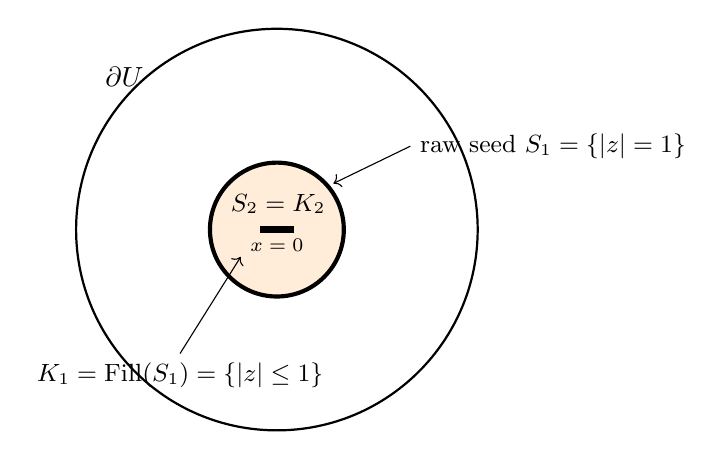
\begin{tikzpicture}[scale=0.85]
% localization boundary
\draw[thick] (0,0) circle (3);
\node at (135:3.22) {$\partial U$};
% filled hull K_1, shaded
\fill[orange!15] (0,0) circle (1);
% raw seed S_1
\draw[line width=1.5pt] (0,0) circle (1);
\draw[<-,shorten <=1.5pt] (40:1.03) -- (32:2.35)
  node[right,align=left] {\small raw seed $S_1=\{|z|=1\}$};
% shaded-hull annotation
\draw[<-,shorten <=1.5pt] (215:0.62) -- (232:2.35)
  node[below,align=left] {\small $K_1=\Fill(S_1)=\{|z|\le1\}$};
% raw seed S_2 inside the hull
\draw[line width=2.6pt] (-0.25,0) -- (0.25,0);
\node[above] at (0.02,0.09) {\small $S_2=K_2$};
% witness point
\fill (0,0) circle (1.3pt);
\node[below,inner sep=2pt] at (0,-0.05) {\scriptsize $x=0$};
\end{tikzpicture}
\caption{The post-fullification merger of Example~\ref{ex:merger} in the
localization $U=\{|z|<3\}$. The raw seeds --- the circle $S_1$ and the segment
$S_2$ --- are disjoint, so every seed-level disjointness audit passes. But the
completion $K_1=\Fill(S_1)$ is the closed unit disk (shaded), which contains
$S_2=K_2$: the completed packets merge. The witness point $x=0$ carries the record
$(1,2,0,\mathrm{ch}_1(0),\mathrm{ch}_2(0))$ with $\mathrm{ch}_1(0)$ the bounded
complementary chamber $\{|z|<1\}$ of $S_1$ and $\mathrm{ch}_2(0)=\textsf{seed}$. By
monotonicity of $\Fill$ the merger persists under every same-label enlargement of
the seeds; only a different typed assignment removes it.}
\label{fig:merger}
\end{figure}

\subsection{The cellwise certificate}\label{subsec:E-cellwise}

The audit clauses of Theorem~\ref{thm:audit} still require computing each completion
and comparing every pair of completions across the localization. The final result of
this section decomposes even this: it confines each packet to its own closed Jordan
cell, inside which the completion is trapped automatically and the port verification
becomes local to the cell. Disjointness of the completions then follows from
disjointness of the cells, which is checked on $N$ disks rather than on
$\binom N2$ pairs of filled hulls.

\begin{proposition}[Cellwise packet-and-port certificate; manuscript Proposition
10.15]\label{prop:cellwise}
Let $N\ge s\ge1$, let $U$ be a Jordan domain, and let
$D_1,\dots,D_N\Subset U$ be pairwise disjoint
closed Jordan disks.  Index the atom packets first.  Suppose every packet
has a nonempty compact connected raw seed
$S_\ell\Subset D_\ell$, the seeds cover the complete frozen inventory,
$\mathcal B_i\subset S_i$ for $1\le i\le s$, and every original atom $A_i$ has an
unprotected point $x_i\in A_i\setminus P_i$
and a Jordan arc $\gamma_i\colon[0,1]\to D_i$ satisfying
\begin{equation}\label{eq:E-arc-condition}
\gamma_i(0)=x_i,
\qquad
\gamma_i\bigl((0,1)\bigr)\subset D_i\setminus S_i,
\qquad
\gamma_i(1)\in\partial D_i
\end{equation}
(condition~(9.11a) of \cite{MWman}). Then $K_\ell=\Fill(S_\ell)\Subset D_\ell$, the
completed packets are pairwise disjoint, every $x_i\in\Exp(A_i,K_i;P_i)$, and the
packet system has simultaneous ports and one common free component; hence
it supplies a protected ribbon-routing certificate and its realized
carrier.
\end{proposition}

\begin{proof}
\emph{Step 1: the completion is trapped in its cell.}
Fix $\ell$. By the Schoenflies theorem, $S^2\setminus D_\ell$ is an open Jordan disk
containing $\infty$, so its planar part $\C\setminus D_\ell$ --- an open disk with
one point removed --- is connected, and it is unbounded. Since
$S_\ell\Subset D_\ell$ means $S_\ell\subset\Int D_\ell$, the exterior
$\C\setminus D_\ell$ is a connected unbounded subset of $\C\setminus S_\ell$ and
therefore lies in the unbounded component $\Omega_\infty(S_\ell)$. Consequently
every bounded component $B$ of $\C\setminus S_\ell$ is disjoint from
$\C\setminus D_\ell$ --- distinct components of $\C\setminus S_\ell$ are disjoint
--- so $B\subset D_\ell$, and $\Fill(S_\ell)\subset D_\ell$. The containment is
compact: a point $x\in\partial D_\ell$ does not lie in $S_\ell\subset\Int D_\ell$,
and every neighborhood of $x$ meets $\C\setminus D_\ell\subset
\Omega_\infty(S_\ell)$; since the component of $\C\setminus S_\ell$ containing $x$
is open and contains a small ball around $x$, that component meets
$\Omega_\infty(S_\ell)$ and hence equals it, so $x\in\Omega_\infty(S_\ell)$ and
$x\notin\Fill(S_\ell)$. Thus $K_\ell=\Fill(S_\ell)\subset\Int D_\ell$, and being
compact, $K_\ell\Subset D_\ell$. The cells are pairwise disjoint, so the completions
are pairwise disjoint, and $D_\ell\Subset U$ gives $K_\ell\Subset U$.

\emph{Step 2: the arc condition certifies exposure.}
Fix $i$. The point $\gamma_i(1)$ lies on the Jordan curve $\partial D_i$, which
bounds the closed Jordan disk $S^2\setminus\Int D_i$ containing $\infty$ in its
interior. Straightening this disk by the Schoenflies theorem \cite{New51} and taking
the preimage of a radius, we obtain a Jordan arc $\beta$ from $\gamma_i(1)$ to
$\infty$ meeting $D_i$ only at $\gamma_i(1)$. Consider the concatenated set
\[
\Gamma\;:=\;\gamma_i\bigl((0,1]\bigr)\,\cup\,\bigl(\beta\setminus\{\infty\}\bigr),
\]
a connected unbounded subset of $\C$. It is disjoint from $S_i$: the piece
$\gamma_i((0,1))$ lies in $D_i\setminus S_i$ by \eqref{eq:E-arc-condition}; the
point $\gamma_i(1)$ lies on $\partial D_i$, which misses $S_i\subset\Int D_i$; and
$\beta\setminus\{\gamma_i(1),\infty\}$ lies in $\C\setminus D_i\subset
\C\setminus S_i$. A connected unbounded subset of $\C\setminus S_i$ lies in the
unbounded component $\Omega_\infty(S_i)$, so in particular
\[
\gamma_i\bigl((0,1]\bigr)\;\subset\;\Omega_\infty(S_i)
\;=\;\C\setminus\Fill(S_i),
\]
that is, $\gamma_i((0,1])$ misses $K_i$. Since $x_i\in A_i\subset S_i\subset K_i$,
this gives
\[
\gamma_i\cap K_i\;=\;\{x_i\} .
\]
The arc $\gamma_i$ maps into $D_i\subset U$, and $x_i\in A_i\setminus P_i$ by
hypothesis, so $\gamma_i$ is precisely an arc of the form read by
\eqref{eq:E-exposure}: every $x_i\in\Exp(A_i,K_i;P_i)$.

\emph{Step 3: assembly.}
The three audit clauses of Theorem~\ref{thm:audit} now hold: clause~(1), because the
seeds are nonempty, compact, connected, and cover the complete frozen inventory by hypothesis;
clause~(2), by Step~1; and clause~(3), by Step~2. Lemma~\ref{lem:port-localization}
turns the individual arcs into pairwise disjoint simultaneous port arcs with
positive-parameter parts in the common complement of the completions, and
Theorem~\ref{thm:audit} certifies that the geometric augmented-packet clauses of
Definition~\ref{def:packet} hold for this assignment. Theorem~\ref{thm:common-domain}
then determines one common free component of $\Omfree$ with simultaneous singleton
ports to every original atom, hence a protected ribbon-routing certificate
and its realized carrier.
\end{proof}

This proposition is sufficient only, and we close the section by marking the
boundary of what it proves, in the discipline of Section~\ref{sec:scope}. The
cellwise certificate solves the planar verification problem once the cells
$D_\ell$, the complete seeds $S_\ell$, and the unprotected arcs $\gamma_i$ are
supplied. The actual virtual theorem contemplated by the source manuscript must
still \emph{construct} those cells, complete seeds, and unprotected arcs, and must
transport them through the final Wave horizon; that construction is posed in
\cite{MWman} only as an open problem, it is not addressed by anything in this paper,
and no clause of Theorem~\ref{thm:audit} or Proposition~\ref{prop:cellwise} is
promoted here to a statement about virtual carriers, the Wave horizon, or Mandelbrot
local connectivity.
% ---- end E:audit ----

% ---- begin G:scope_v2 ----
\section{Scope, interfaces, and next gates}
\label{sec:scope}

\subsection{What the finite theory closes}

For a completely specified finite inventory, the paper closes the planar
routing problem at three levels.
\begin{enumerate}
\item A protected ribbon-routing certificate is realized by a full carrier,
with the declared prime-end chains, distinctness, and cyclic order preserved
(Theorem~\ref{thm:realization}).
\item Existence of such a certificate is equivalent to one component of the
frozen free domain having simultaneous singleton ports
(Theorem~\ref{thm:free-component}).
\item Theorem~\ref{thm:audit} gives each fixed packet assignment a finite
audit with three monotone-persistent failure modes.
Theorem~\ref{thm:common-domain} and Proposition~\ref{prop:cellwise}
provide positive sufficient tests.
\end{enumerate}
The attachment ledger additionally decides when replacing the certificate
tree by a more general continuum connector preserves fullness
(Theorem~\ref{thm:separation-budget} and
Corollary~\ref{cor:full-connector-traces}).

These conclusions are invariant under orientation-preserving conformal
changes of the Jordan localization.  They require no local connectivity of
the atoms, no boundary parametrization, no presumed ray landing, and no
metric width estimate.

\subsection{What remains outside the theorem}

The finite theory does not supply the data it audits.  In particular it does
not construct:
\begin{enumerate}
\item a forward-coherent protected inventory at all depths;
\item a virtual carrier or a Wave horizon;
\item an analytic correspondence, covering action, or immersion action on
such a horizon;
\item a uniform incidence bound, marked-width estimate, or compression
mechanism; or
\item a proof of local connectivity for any new Mandelbrot parameter.
\end{enumerate}
The direct-decoration rooted-end compactification and its finite carrier
application belong to the companion paper \cite{Wes26}; importing that
application here would duplicate its principal results without closing any
of the infinite gates above.

\subsection{Three next research gates}

The results isolate three concrete directions in which a future argument can
advance.

\paragraph{The inverse-envelope gate.}
Theorem~\ref{thm:nested-limit-stability} shows that decreasing full connector
envelopes with connected traces pass safely to the limit.  A dynamical
construction of such envelopes, compatible with pullback and with one frozen
family of relative collar tails, would bypass the two Hausdorff defects of
Warning~\ref{warn:compactness-gate}.  What is missing is the construction,
not another compactness extraction.

\paragraph{The quantitative routing gate.}
The exact free-component criterion is qualitative.  It neither bounds the
number of sides of the ribbon tree nor supplies a modulus, width, or
incidence estimate.  Any application requiring analytic compression must
augment a topological certificate by a quantitative routing theorem inside
the same frozen component.  The separation ledger identifies the invariant
that such a theorem must preserve, but does not provide the estimate.

\paragraph{The coherent-marking gate.}
Prime-end survival here is finite-family survival.  Passing to infinitely
many accesses requires a coherent choice of null chains and relative
collar tails whose truncations remain compatible across levels.  Pairwise
distinctness at every finite stage is insufficient by itself: impressions
may overlap in the atoms, and collar widths may collapse.  A successful
coherence theorem must therefore be formulated in the complement, in terms
of relative tails and selected sides, rather than as pointwise separation of
impressions.

These gates are intentionally stated as proof obligations, not conjectural
consequences of the present paper.  The value of the finite theory is that a
future construction can now be tested against exact planar conditions, and a
failure produces a persistent witness rather than an ambiguous instruction
to ``choose a better hull.''
% ---- end G:scope_v2 ----

\section*{Acknowledgments}
AI-assisted drafting and citation checking were used.  The author
independently verified and assumes responsibility for all mathematical
statements, proofs, and references.

\appendix

\section{Provenance and statement crosswalk}\label{sec:crosswalk}

The certificate, criterion, and packet results originated in the source
research manuscript \cite{MWman}.  This draft corrects the slit statement,
uses null crosscut chains and relative collar tails throughout, repairs the
single-atom construction, and adds the separation ledger, the sharp
Hausdorff-limit example, and nested-limit stability.  No statement labeled
open or conditional in the source has been promoted.

\begin{center}
\small
\begin{tabularx}{\textwidth}{@{}P{0.35\textwidth}P{0.22\textwidth}Y@{}}
\toprule
Present result & Source & Status in this paper\\
\midrule
Theorem~\ref{thm:no-least} & Theorem 6.12 & extracted\\
Proposition~\ref{prop:access-collision} & Proposition 6.15 & extracted\\
Definition~\ref{def:certificate} & Definition 10.1 &
relative-tail and incidence conventions made explicit\\
Lemma~\ref{lem:tree-full} & Lemma 10.2 & two proofs supplied\\
Lemma~\ref{lem:crosscut-survival} & Lemma 10.3 &
relative-tail formulation\\
Theorem~\ref{thm:realization} & Theorem 10.4 &
proof synchronized with corrected conventions\\
Proposition~\ref{prop:naturality} & Proposition 10.5 & extracted\\
Theorem~\ref{thm:separation-budget} & Draft II &
classical duality/Mayer--Vietoris consequence, packaged for carriers\\
Corollary~\ref{cor:full-connector-traces} & Draft II &
classical zero-defect consequence, packaged for carriers\\
Proposition~\ref{prop:trace-birth} & Draft II &
Hausdorff-limit separation example proved in this draft\\
Theorem~\ref{thm:nested-limit-stability} & Draft II &
decreasing-envelope theorem proved in this draft\\
Lemma~\ref{lem:slits} & Lemma 10.7 &
repaired; see Remark~\ref{rem:repair}\\
Theorem~\ref{thm:free-component} & Theorem 10.8 &
proof rebuilt around the repaired slit lemma; $s=1$ included\\
Definition~\ref{def:packet} & Definition 10.9 &
compact atom--tail blocks and named compact obstacle pieces\\
Lemma~\ref{lem:packets} & Lemma 10.10 &
compacta duality made explicit\\
Theorem~\ref{thm:common-domain} & Theorem 10.11 & extracted\\
Lemma~\ref{lem:fill-absorption} & Lemma 10.12 & extracted\\
Lemma~\ref{lem:port-localization} & Lemma 10.13 & extracted\\
Theorem~\ref{thm:audit} & Theorem 10.14 & extracted\\
Proposition~\ref{prop:cellwise} & Proposition 10.15 & extracted\\
\bottomrule
\end{tabularx}
\end{center}

Examples~\ref{ex:no-common-component} and~\ref{ex:merger}, together with
Section~\ref{sec:comparison}, are expository additions.  The
direct-decoration application formerly included in Draft~I has been removed
because its strengthened form is the subject of the companion paper
\cite{Wes26}.

\begin{thebibliography}{99}

\bibitem{Bor31}
K.~Borsuk,
\emph{Quelques th\'eor\`emes sur les ensembles unicoh\'erents},
Fund. Math. \textbf{17} (1931), 171--209.

\bibitem{DH85}
A.~Douady and J.~H.~Hubbard,
\emph{On the dynamics of polynomial-like mappings},
Ann. Sci. \'Ec. Norm. Sup\'er. (4) \textbf{18} (1985), 287--343,
doi:10.24033/asens.1491.

\bibitem{DHOrsay}
A.~Douady and J.~H.~Hubbard,
\emph{\'Etude dynamique des polyn\^omes complexes, Parties I--II},
Publications Math\'ematiques d'Orsay 84-02 (1984) and 85-04 (1985).

\bibitem{Dud25}
D.~Dudko,
\emph{On the MLC conjecture and the renormalization theory in complex
dynamics},
to appear in the Proceedings of the ICM 2026,
arXiv:2512.24171v1, submitted 30 December 2025.

\bibitem{Eil36}
S.~Eilenberg,
\emph{Sur les espaces multicoh\'erents. I},
Fund. Math. \textbf{27} (1936), 153--190.

\bibitem{Hat02}
A.~Hatcher,
\emph{Algebraic Topology},
Cambridge University Press, Cambridge, 2002.

\bibitem{KKL26}
J.~Kahn, A.~Kapiamba, and M.~Lyubich,
\emph{MLC for parabolically bounded primitive renormalization},
arXiv:2606.27272v1, submitted 25 June 2026.

\bibitem{KL08}
J.~Kahn and M.~Lyubich,
\emph{A priori bounds for some infinitely renormalizable quadratics.
II. Decorations},
Ann. Sci. \'Ec. Norm. Sup\'er. (4) \textbf{41} (2008), 57--84,
doi:10.24033/asens.2063.

\bibitem{Jan15}
Z.~Janiszewski,
\emph{O rozcinaniu p\l aszczyzny przez kontinua}
[French summary: \emph{Sur les coupures du plan faites par des continus}],
Prace Matematyczno-Fizyczne \textbf{26} (1915), 11--63.

\bibitem{Moo25}
R.~L.~Moore,
\emph{Concerning upper semi-continuous collections of continua},
Trans. Amer. Math. Soc. \textbf{27} (1925), 416--428,
doi:10.1090/S0002-9947-1925-1501320-8.

\bibitem{Mul22}
A.~M.~Mullikin,
\emph{Certain theorems relating to plane connected point sets},
Trans. Amer. Math. Soc. \textbf{24} (1922), 144--162,
doi:10.2307/1989040.

\bibitem{MWman}
M.~R.~Wesney,
\emph{A marked-width reduction of Mandelbrot local connectivity},
unpublished research manuscript, 2026 (build of 2026-07-27).

\bibitem{New51}
M.~H.~A.~Newman,
\emph{Elements of the Topology of Plane Sets of Points},
2nd ed., Cambridge University Press, Cambridge, 1951.

\bibitem{Pom92}
Ch.~Pommerenke,
\emph{Boundary Behaviour of Conformal Maps},
Grundlehren der mathematischen Wissenschaften \textbf{299},
Springer-Verlag, Berlin, 1992.

\bibitem{Spa66}
E.~H.~Spanier,
\emph{Algebraic Topology},
McGraw--Hill, New York, 1966.

\bibitem{Wes26}
M.~R.~Wesney,
\emph{The direct-decoration rooted-end compactification},
companion manuscript in preparation, 2026.

\bibitem{Why42}
G.~T.~Whyburn,
\emph{Analytic Topology},
American Mathematical Society Colloquium Publications \textbf{28},
American Mathematical Society, New York, 1942.

\end{thebibliography}

\end{document}
